%%%%%%%%%%%%%%%%%%%%%%%%%%%%%%%%%%%%%%%%%%%%%%%%%%%%%%%%%%%%%%%%%%%
%%%
%%%  Bachelor thesis
%%%
%%%  English Title: 
%%%      LaTeX Template for Graduate Research Thesis
%%% 
%%%                                          written by Kentaro UNO 
%%%
%%%  2021.02.12 Updated by Kentaro UNO to design this as an English template
%%%  2022.12.26 Updated by Kentaro UNO to build this template in overleaf
%%%
%%%%%%%%%%%%%%%%%%%%%%%%%%%%%%%%%%%%%%%%%%%%%%%%%%%%%%%%%%%%%%%%%%%%

\documentclass[a4paper,12pt]{./include/ethesis_gen} % use the style file created by Dr. Genya Ishigami

%%% AMS's Latex math and symbol library
\usepackage{amsmath}
\usepackage{amssymb}
% \usepackage{algorithm}
% \usepackage{algpseudocode}

%%% subfigure
%\usepackage{subfigure}
%\usepackage{./include/subfigure} %subfigure is not recommended to use. You can use minipage.

%%% caption related
\usepackage{caption}
\usepackage{subcaption}
\usepackage[subrefformat=parens]{subcaption} %\subref command with brakets.
\captionsetup{compatibility=false}

%%% etc
\usepackage{color}
\usepackage{setspace}
%\usepackage{indentfirst}%foce indent
\usepackage{otf}
%\if0
\usepackage{cite} % indexing reference
\usepackage{multirow} 
\usepackage{comment} % activate comment command in .tex file.
\usepackage{tabularx}
\usepackage{epsf}

%% Uncomment if you need
\usepackage{siunitx} % use SI unit
% \usepackage{bm} % use bold font for vector
% \usepackage{arydshln} % use dashline in table or matrix
\usepackage{physics} % useful for writing formulas

\usepackage{textcomp}
\usepackage{ascmac}
\renewcommand\thefootnote{\arabic{footnote}}

%%% Table related
\usepackage{multirow}
\usepackage[table]{xcolor}

%%% Algorithm related %%%
\usepackage{algorithm}
\usepackage{algpseudocode}
\usepackage{xcolor}

%%% package for Hyper link, added by Kentaro UNO 2020.3.21
\usepackage[dvipdfmx]{hyperref,graphicx} %{graphicx}:png can be inserted
% Japanese Garbling Prevention Package
\usepackage{pxjahyper}
\hypersetup{% hyperref option list
% setpagesize=true,
pdfborder={2 2 1},
colorlinks=true,
linkcolor=black,
citecolor=black,
urlcolor=black,
%%% Uncommenting below, the link boader becomes a dotted square
% pdfborderstyle=/S/D/D[3 2]/W 1,
%%% Uncommenting below, the link boader becomes underlined
% pdfborderstyle={/S/U/W 1},
%%% You can goolge "\hypersetup option" for more editable options,
% linkcolor=blue,
% citecolor=red,
hidelinks, % do not show frame border of links
}

%%%%%%%%%%%%%%%%				
%\fi

%%%%%%%%%%%%%%%%%%%%%%%%%%%%%%%%%%%%%%%%
%%%  TeX macro command settings
%%%%%%%%%%%%%%%%%%%%%%%%%%%%%%%%%%%%%%%%
%%%%%%%%%%%%%%%%%%%%%%%%%%%%%%%%%%%%%%%%%%%%%%%%%%%%%%%%%%%%%%%%%%%%%%
%%
%%   macrosForEThesis.tex
%%   -------------------
%%
%%   Title: LaTeX macro file for the English Thesis
%%   
%%   
%%   Belief:
%%   1."Fig. 1: ~~~", "Table 1: ~~~" are for the figure and table citation.
%%   2. add the config to read the source code file (hello.c) and visualize it. 
%%
%%   Change Log:
%%   2020.11.26 Initial creation by Kentaro UNO
%%
%%   Contact:
%%   Please contact the author Kentaro UNO (unoken.astro@gmail.com) if
%%   you have a problem
%%
%%%%%%%%%%%%%%%%%%%%%%%%%%%%%%%%%%%%%%%%%%%%%%%%%%%%%%%%%%%%%%%%%%%%%%

%%% useful command
\newcommand{\n}{\nonumber \\}
\newcommand{\p}{\partial}
\newcommand{\bs}[1]{\boldsymbol{#1}}
\newcommand{\II}{I\negthinspace I}
\newcommand{\III}{I\negthinspace I\negthinspace I}
\newcommand{\mbm}[1]{\mbox{\protect \boldmath $#1$}}

%%%%%%%%%%%%%%%%%%%%%%%%%%%%%%%%%%%%%%%%
%%%  config for citation of figures, tables, and equations
%%%  to use English for all. 
%%%  2020.01.29 modified by Kentaro UNO
%%%%%%%%%%%%%%%%%%%%%%%%%%%%%%%%%%%%%%%%

%%% figure and table
\captionsetup{compatibility=false}
%
\renewcommand{\figurename}{Fig.~\hspace{-.2em}}   
\renewcommand{\tablename}{Table~\hspace{-.2em}}

\captionsetup[figure]{format=plain,labelformat=simple,labelsep=colon,font=small}
\captionsetup[table]{format=plain,labelformat=simple,labelsep=colon,font=small}

\newcommand{\bhline}[1]{\noalign{\hrule height #1}} % bhlineコマンドの設定

%%% citation command for figures, tables, and equations
\newcommand{\fig}[1]{Fig.~\ref{#1}}
\newcommand{\subfig}[2]{Fig.~\ref{#1}\subref{#2}}
\newcommand{\fign}[1]{\ref{#1}}
\newcommand{\tb}[1]{Table~\ref{#1}}
\newcommand{\tabn}[1]{\ref{#1}}
\newcommand{\eq}[1]{Eq.~(\ref{#1})}
\newcommand{\eqn}[1]{(\ref{#1})}

%%% citation command for chapters, sections, and appendixes
\newcommand{\chap}[1]{Chap.~\ref{#1}}
\newcommand{\sect}[1]{Sect.~\ref{#1}}
\newcommand{\subsect}[1]{Sect.~\ref{#1}}
\newcommand{\app}[1]{Appnd. ~\ref{#1}}

%%% visualize a figure and table in a row
\makeatletter
\newcommand{\figcaption}[1]{\def\@captype{figure}\caption{#1}}
\newcommand{\tblcaption}[1]{\def\@captype{table}\caption{#1}}
\makeatother

%%%%%%%%%%%%%%%%%%%%%%%%%%%%%%%%%%%%%%%%
%%%  ソースコードの引用スタイルの設定
%%%  2020.01.24 added by Kentaro UNO
%%%%%%%%%%%%%%%%%%%%%%%%%%%%%%%%%%%%%%%%
\usepackage{listings} %日本語のコメントアウトをする場合はjlistingが必要
%ここからソースコードの表示に関する設定
\definecolor{gray}{rgb}{0.9,0.9,0.9}
\lstset{
  backgroundcolor=\color{gray}, % choose the background color; you must add \usepackage{color} or \usepackage{xcolor}; should come as last argument
  basicstyle={\small\ttfamily}, % the style of the fonts that are used for the code
  identifierstyle={\small}, % main()の''main''等のスタイル
  commentstyle={\small\itshape}, %//comment 等のスタイル
  keywordstyle={\small}, % int mainの''int''等のスタイル
  ndkeywordstyle={\small},
  stringstyle={\small\ttfamily},  % string literal style -> % printf(''Hello'')の''''で囲まれた部分のスタイル
  %frame={tb},
  breaklines=true, % sets automatic line breaking
  columns=[l]{fullflexible},
  numbers=left, % where to put the line-numbers; possible values are (none, left, right)
  numberstyle={\scriptsize}, % the style that is used for the line-numbers
  stepnumber=1, % the step between two line-numbers. If it's 1, each line will be numbered
  numbersep=1zw, % 行数字とコードの間のマージン
  xrightmargin=0zw, % 表示個所の右側マージン
  xleftmargin=2zw,  % 表示個所の左側マージン
  rulecolor=\color{black},         % if not set, the frame-color may be changed on line-breaks within not-black text (e.g. comments (green here))
  showspaces=false,                % show spaces everywhere adding particular underscores; it overrides 'showstringspaces'
  showstringspaces=false,          % underline spaces within strings only
  showtabs=false,                  % show tabs within strings adding particular underscores
  lineskip=-0.5ex % codeの行間の設定
}

\def\epsgaiji#1{\leavevmode\kern-0.025zw\raise-.37zh\hbox{%
  \epsfile{file=#1,width=1.05zw}}\kern-0.025zw}
%\newcommand{\dfrac}[2]{\frac{\displaystyle{#1}}{\displaystyle{#2}}}
\newcommand{\MARU}[1]{{\ooalign{\hfil#1\/\hfil\crcr\raise.167ex\hbox{\mathhexbox20D}}}}

%%%  % made a macros.tex to wrap the settings by Kentaro UNO 2021.2.12			

%%%%%%%%%%%%%%%%%%%%%%%%%%%%%%%%%%%%%%%%%%%%
%%%%% text vertical size %%%%%%%%%%%%%%%%%%%
%%%%%%%%%%%%%%%%%%%%%%%%%%%%%%%%%%%%%%%%%%%%
\topmargin -25.4mm		%%%%% 上部余白なしにしておきヘッダ領域を設ける
\headheight 20.5mm		%%%%% \headheight + \headsep = 25mm, 上部余白20mmに
\headsep 7mm			%%%%% しなければいけないらしいが7.5mm大きめにします.
\textheight 242mm		%%%%% 297 - (下部余白27.5mm) - (上部部余白27.5mm) 
\footskip 13.75mm		%%%%% 下部中央(27.5/2=13.75mm)にページ番号

%%%%%%%%%%%%%%%%%%%%%%%%%%%%%%%%%%%%%%%%
%%%%% text lateral size %%%%%%%%%%%%%%%%
%%%%%%%%%%%%%%%%%%%%%%%%%%%%%%%%%%%%%%%%
\textwidth 155mm		%%% 奇数ページ右余白25mm,偶数ページ右余白30mm
\oddsidemargin  4.6mm		%%% 25.4mm + x	奇数ページ左余白30mm
\evensidemargin -0.4mm  	%%% 25.4mm + x	偶数ページ左余白25mm

%%%%%%%%%%%%%%%%%%%%%%%%%%%%%%%%%%%%%%%%
%%%%% 文字横間隔,行間隔 %%%%%%%%%%%%%%%
%%%%%%%%%%%%%%%%%%%%%%%%%%%%%%%%%%%%%%%%
\renewcommand{\baselinestretch}{1.2}	%% すべての行間.デフォルトは1
\baselineskip 4.0ex			%% 連続する文章の行間
\kanjiskip=0.15pt plus 0pt minus 3pt	%% 文字間隔
\xkanjiskip=0.15pt plus 0pt minus 3pt	%% 文字間隔
\parindent 12pt				%% 段落の字下げ(12pt=1字分)
%\parskip 1pt 				%% 段落の間隔

%%%%%%%%%%%%%%%%%%%%%%%%%%%%%%%%%%%%%%%%
%%%%% 図・表・式のキャプション関係 %%%%%
%%%%%%%%%%%%%%%%%%%%%%%%%%%%%%%%%%%%%%%%
%%%表題形式の変更(P58)
\makeatletter
\renewcommand{\section}{\@startsection{section}{1}{0mm}{1mm}{1mm}{\raggedright\bfseries\Large}}
\renewcommand{\subsection}{\@startsection{subsection}{1}{0mm}{1mm}{1mm}{\raggedright\bfseries\normalsize}}
\makeatother


%%%箇条書きレイアウトパラメータ(P238)\listのみ
\leftmargini    = 10mm
\parskip        = 0mm

%図表環境問題点の改善策(P263)
\setcounter{topnumber}{100}
\setcounter{bottomnumber}{100}
\setcounter{totalnumber}{100}
\renewcommand{\topfraction}{1.0}
\renewcommand{\bottomfraction}{1.0}
\renewcommand{\textfraction}{0.0}
\renewcommand{\floatpagefraction}{0.0}

%図表環境レイアウト(P265)
\intextsep  =  2mm



%脚注*表示
\renewcommand\thefootnote{*\arabic{footnote}}
%\newcommand{\Gcenter}[2]{
%	\dimen0=\ht\strutbox
%	\advance\dimen0\dp\strutbox
%	\multiply\dimen0 by#1
%	\divide\dimen0 by2
%	\advance\dimen0 by-.5\normalbaselineskip
%	\raisebox{-\dimen0}[0pt][0pt]{#2}
%	}

\abovecaptionskip  1mm     %キャプションの上余白
\belowcaptionskip  1mm     %キャプションの下余白


%%%%%%%%%%%%%%%%%%%%%%%%%%%%%%%%%%%%%%%%
%%%  文書部分の開始 
%%%%%%%%%%%%%%%%%%%%%%%%%%%%%%%%%%%%%%%%

%%%%%%%%%%%%%%%%%%%%
%%%   表題   
%%%%%%%%%%%%%%%%%%%%
\title{ \vspace{-30mm}
{\Large \bf Graduation Thesis} \\
{\Large \bf School of Engineering, Tohoku University} \\
\vspace{20mm}
{\Huge \bf Self-Recognition-based of Modular Legged Robot} \\
\vspace{60mm}
}

\author{
{\Large \bf Department of Mechanical and Aerospace Engineering}\\
{\Large \bf Space Robotics Laboratory}\vspace{25mm}\\
{\LARGE \bf C0TB1716 Tharit Sinsunthorn}\\
{\Large \bf (March, 2024)} \vspace{10mm}}
\date{}

%%%%%%%%%%%%%%%%%%%%
%%%   本文開始   
%%%%%%%%%%%%%%%%%%%%
\begin{document}
\maketitle
\thispagestyle{empty}
~~\newpage

%%%%%%%%%%%%%%%%%%%%
%%%   Abstract 
%%%%%%%%%%%%%%%%%%%%
\pagenumbering{roman}
%%%% Abstrast's pages are set MYHEADINGS mode
\pagestyle{myheadings}\def\Vec#1{\mbox{\boldmath $#1$}}
\begin{center}
  {\large \bf Self-Recognition-based of Modular Legged Robot} 
  
  {\large \bf} Tharit Sinsunthorn
\end{center}

\begin{center}
  \LARGE \bf Abstract
\end{center}

In the expansive domain of lunar exploration, where the rugged lunar terrain and harsh environmental conditions present formidable challenges, the pursuit of innovative robotic solutions has intensified. Modular legged robots have emerged as a promising frontier, offering unparalleled adaptability and maneuverability in navigating the diverse lunar landscapes.

This thesis introduces "Moonbot", a modular legged robot to transcend the limitations of traditional lunar exploration missions. Developed as part of the prestigious Moonshot project led by the Space Robotics Laboratory at Tohoku University. Moonshot project has a strong aiming to develop a modular robot with the implementation of plug-and-play AI system for the propose of solar panels and lunar based construction. Henceforth, Moonbot stands as the pioneering prototype, embodying and extending the conceptual framework for robotic operations across lunar terrains. Its inception marks a pivotal moment in the evolution of robotic exploration, illuminating new pathways and possibilities for traversing and navigating the lunar landscape with unprecedented efficiency and adaptability.

Moonbot's innovative design is characterized by its self-recognition-based motion control capabilities, allowing dynamic adaptability to various leg configurations, from solitary to quadrupedal stances. Central to its design philosophy is a flexible structure, facilitated by magnetic connections between modular components, enabling rapid reconfiguration to meet evolving mission requirements.

Within the Moonshot project framework, Moonbot serves as a pioneering platform for testing and validating novel robotic technologies for lunar exploration and lunar base construction. Its modularity extends to independent leg controllers seamlessly integrated within the Robot Operating System 2 (ROS2) framework, ensuring seamless communication and precise control.

As Moonbot continues to undergo rigorous testing and refinement, it represents a significant leap forward in the quest for innovative robotic solutions for lunar exploration and beyond. With its adaptable design and robust capabilities, Moonbot embodies the spirit of exploration and innovation driving the Moonshot project, paving the way for future advancements in lunar robotics and space exploration.

\bigskip



\clearpage


% Add more content as needed


\thispagestyle{myheadings}

%%%%%%%%%%%%%%%%%%%%
%%%   目次 
%%%%%%%%%%%%%%%%%%%%
%%% table's pages are set headings mode

\pagestyle{headings}
\setcounter{page}{1}%目次はローマ数字でi頁からナンバリング
\pagenumbering{roman}
\tableofcontents
\listoftables
\listoffigures

%%%%%%%%%%%%%%%%%%%%
%%%   各章 
%%%%%%%%%%%%%%%%%%%%
\pagestyle{headings}
\chapter{Introduction}
\setcounter{page}{1} %本文はアラビア数字で再度1頁からナンバリング
\pagenumbering{arabic}
\label{cha:intro}
%%%%%%%%%%%%%%%%%%%%%%%%%%%%%%%%%%%%%%%%%%%%%%%%%%%%%%%%%
%%%
%%%  Chapter 1
%%%  Introduction
%%%
%%%%%%%%%%%%%%%%%%%%%%%%%%%%%%%%%%%%%%%%%%%%%%%%%%%%%%%%%
In the ambitious pursuit of lunar exploration, the traditional boundaries of robotics are being redefined. The quest for a robot capable of navigating the hazardous lunar environment has led to the development of Moonbot, a modular legged robot designed to transcend the limitations of conventional rover-based exploration. The essence of Moonbot lies in its ability to dynamically adapt and respond to the challenges presented by the lunar terrain.\\

%%%%% BACKGROUND %%%%%
\section{Background}\label{sec:background}
\indent
Lunar exploration has long captured the imagination of humanity. From the Apollo missions \cite{apollo} of the 20th century to the more recent lunar rovers, our quest to uncover the secrets of the Moon has driven technological innovation and expanded our understanding of space.

As we look towards the future, the vision of establishing a permanent human presence on the Moon looms ever larger. Central to this vision is the construction of lunar bases, which will serve as hubs for scientific research, and resource utilization, and even as launch pads for missions deeper into space. However, the harsh and unforgiving lunar environment presents formidable challenges for such endeavors.

\begin{figure}[h]
  \centering
  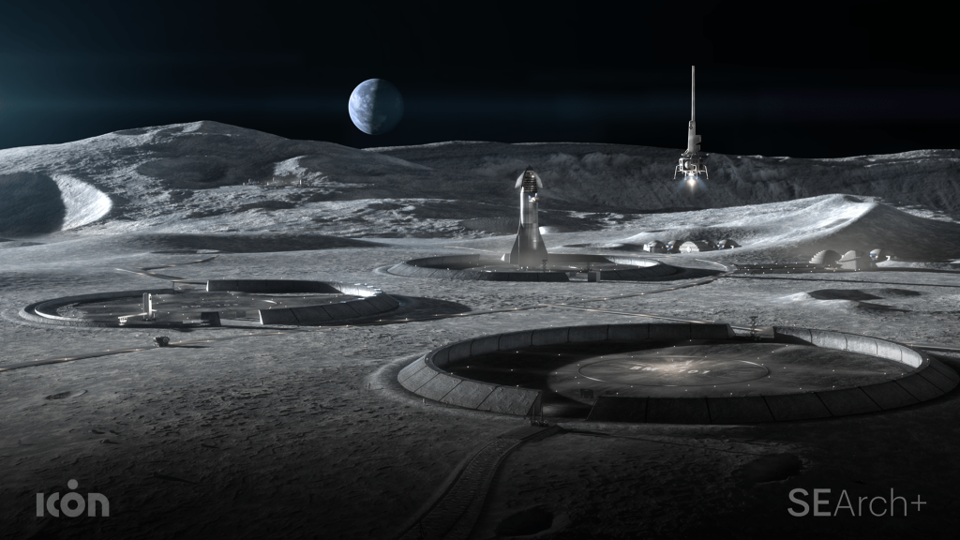
\includegraphics[width=140mm]{./fig/intro/lunarconstruct.png}
  \vspace{2mm}
  \caption{NASA’s Moon to Mars Autonomous Construction Technologies project to advance space-based construction capabilities for long-duration exploration missions on the Moon or Mars. \cite{nasa_construct}}\label{lunar construct}
\end{figure}

In the realm of space robotics research, modular robots, \cite{modularity}, \cite{electrovoxel} emerge as a transformative concept, reshaping our approach to space exploration. A modular robot is a versatile robotic system composed of interchangeable and reconfigurable modules that can be assembled in various configurations to adapt to different tasks and environments. Modular robots have been introduce to space robotics \cite{worms} marks a significant shift, providing unprecedented flexibility and adaptability for the challenges posed by extraterrestrial terrains.

In this thesis, we explore the development and capabilities of Moonbot, a modular legged robot designed for lunar exploration and base construction, following the target of Moonshot Project, Self-evolving AI Robot System for Lunar Exploration and Human Outpost Construction \cite{moonshotGoal3B}. Through a combination of advanced control algorithms, Moonbot aims to push the boundaries of what is possible in extraterrestrial robotics. By harnessing the power of modular design and cutting-edge technology, we strive to pave the way for a new era of lunar exploration and human settlement.
%%%%% BACKGROUND %%%%%

%%%%% LEGGED vs WHEELED %%%%%
\section{Legged vs Wheeled}
Researchers are increasingly considering a shift from wheeled to legged robotic system \cite{spacebok}, particularly in environments where the terrain presents uncertainties. Although wheeled vehicles dominate exploration beyond Earth, this trend might be evolving. While wheels are effective on celestial bodies like the Moon and Mars, other challenging environments, such as smaller moons and asteroids, demand more adaptable solutions. In these low-gravity settings, robots navigating uneven terrain face the possibility of entering prolonged flight phases, a potentially hazardous situation for robots unprepared for such conditions. Below, we explore some of these advantages.\\

\begin{figure}[h]
  \centering
  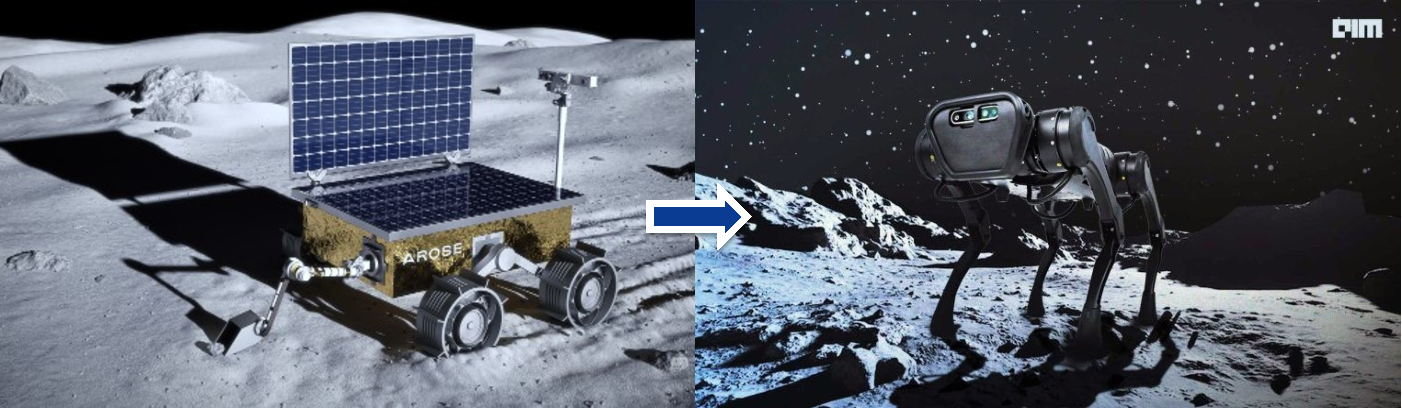
\includegraphics[width=150mm]{./fig/intro/leggedvswheeled.pdf}
  \vspace{2mm}
  \caption{Development of space rover and space legged robot.}\label{fig1}
\end{figure}

\subsection{Mobility}
Legged robots offer superior mobility compared to wheeled robots due to their inherent omni-directional nature. This means that a legged robot can alter its direction independently of the main body axis simply by adjusting its footholds. In contrast, a traditional wheeled robot would need to perform specific maneuvers to change its direction.

Moreover, a legged robot can manipulate its body's movement and orientation while preserving footholds through adjustments in leg extension. This characteristic grants the robot an additional six degrees of freedom (DOF) for its body. It's important to note that while a wheeled robot with traction and directional motors can enhance its directionality, this often comes with the drawback of increased system complexity. Some robots also utilize specialized wheels, such as the ilonator wheel \cite{omniwheel}, to achieve omnidirectionality, but this is typically effective only on flat surfaces.

\subsection{Overcoming Obstacles}
A legged robot has the capability to surmount obstacles situated below its maximum ground clearance by stepping on them. In contrast, a wheeled robot can only navigate obstacles with heights up to half of its wheel radius \cite{mckerrow}. Tracks, which are composed of a virtual wheel with a radius equal to half the track length, allow tracked vehicles to overcome higher obstacles compared to wheeled ones, albeit requiring substantial body motions.

\subsection{Active Suspension}
A legged robot inherently incorporates an active suspension system by adjusting the lengths of its legs in response to terrain irregularities. This capability enables a legged robot to traverse highly uneven terrain while maintaining a level body, ensuring smooth and comfortable motion for riders. In contrast, a wheeled robot keeps its body parallel to the terrain and experiences comparable tilts to the ground.

\subsection{Natural Terrain}
Wheeled vehicles demand costly, consistently paved surfaces for efficient movement. In contrast, legged systems, in principle, do not necessitate prepared terrain like their wheeled counterparts. They can navigate sandy, muddy, rigid, and soft terrains with comparable efficiency. Additionally, legged systems do not rely on continuous terrain for movement, providing another advantage.

\subsection{Slippage and Jamming}
Wheeled vehicles often encounter difficulties moving in soft terrain as their wheels tend to sink. In contrast, a leg, when placed vertically on the ground, only compresses the soft ground in a single direction. Vertical leg lifting avoids interference with the ground, and when the body is in motion, the feet rotate around their joints, preventing legs from interacting with the ground and causing jamming issues. This holds true for vehicle slippage during forward or backward propulsion.

\subsection{Environment Damage}
Legged robots necessitate specific points of contact with the ground, whereas wheeled or tracked vehicles rely on continuous paths along the ground. As a result, legged robots have reduced ground contact compared to conventional vehicles, leading to diminished environmental impact.

%%%%% LEGGED vs WHEELED %%%%%

%%%%% Potential of Legged Robots for Planetary Exploration %%%%%
\section{Legged Robots for Planetary Exploration}
Legged robots' capability to navigate diverse and unknown terrains, surmount obstacles, and employ discrete ground contact points positions them as ideal candidates for planetary exploration. Specific robots have been purposefully designed and tested for such applications, including: (a) the AMBLER, created by Carnegie-Mellon University with NASA funding, serving as an experimental platform for technology development related to potential Mars missions \cite{bares}.\\

\begin{figure}[h]
  \centering
  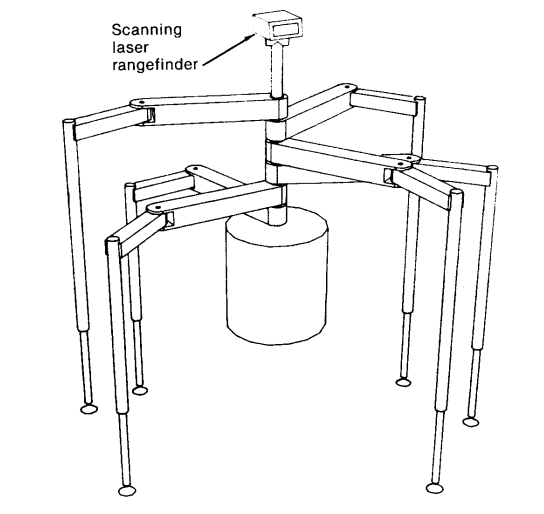
\includegraphics[width=70mm]{./fig/intro/ambler.png}
  \vspace{2mm}
  \caption{Sketch of the AMBLER robot. \cite{bares}}\label{fig ambler}
\end{figure}
%%%%% Potential of Legged Robots for Space Exploration %%%%%

%%%%% Modular Robot %%%%%
\section{Modular Robots: Versatile Solutions for Robotics}

Modular robots represent a fascinating approach to robotics design, offering versatility, adaptability, and scalability in various applications. These robots consist of individual modules or units that can be reconfigured and assembled into different shapes and configurations to suit specific tasks and environments. This modular design allows for flexibility in robot morphology, enabling robots to adapt to diverse operating conditions and perform a wide range of tasks.

\begin{itemize}
    \item \textbf{Versatility}: Modular robots can be reconfigured into various shapes and configurations, allowing them to adapt to different tasks and environments.
    
    \item \textbf{Adaptability}: The ability to dynamically adjust robot morphology enables modular robots to traverse diverse terrain, navigate obstacles, and access hard-to-reach areas.
    
    \item \textbf{Scalability}: Modular design facilitates scalability, allowing robots to be easily expanded or downsized by adding or removing modules as needed.
    
    \item \textbf{Redundancy and Fault Tolerance}: Modular robots inherently offer redundancy and fault tolerance, as module failure or damage can be mitigated by redistributing or replacing modules.
    
    \item \textbf{Resilience}: The ability to reconfigure and adapt to changing conditions enhances the resilience of modular robots, making them suitable for operation in remote and hazardous environments.
\end{itemize}

% In the context of space exploration, where the environment is often harsh, unpredictable, and challenging to navigate, modular robots hold significant promise. The ability to reconfigure robot morphology on-demand can be particularly advantageous for traversing uneven terrain, navigating obstacles, and accessing hard-to-reach areas. By adjusting their configuration, modular robots can optimize their locomotion capabilities to suit the terrain, whether it's rocky, sandy, or steep.

% The lunar surface, with its rugged terrain and varied topography, presents numerous challenges for robotic exploration. Modular robots offer a compelling solution for lunar exploration missions, as their adaptable design allows them to navigate the lunar landscape with agility and resilience. By reconfiguring their morphology to match the terrain, modular robots can traverse crater-like surfaces, scale rocky inclines, and explore lunar caves and crevices.

Moonbot, our modular legged robot designed for space exploration, exemplifies the synergy between modular robotics and lunar exploration. Equipped with a modular architecture, Moonbot is a significant prototype for future lunar exploration mission.

In the event of module failure or damage, the robot can dynamically reconfigure itself by redistributing or replacing modules, ensuring continuity of operation and mission success.

In summary, modular robots represent a paradigm shift in robotics design, offering unparalleled versatility, adaptability, and resilience for lunar exploration and beyond. With their ability to navigate challenging terrain and withstand harsh environmental conditions, these robots hold immense potential to advance our understanding of the Moon and pave the way for future human exploration and habitation.

\begin{figure}[t]
    % \begin{subfigure}{0.45\textwidth}
    %     \centering
    %     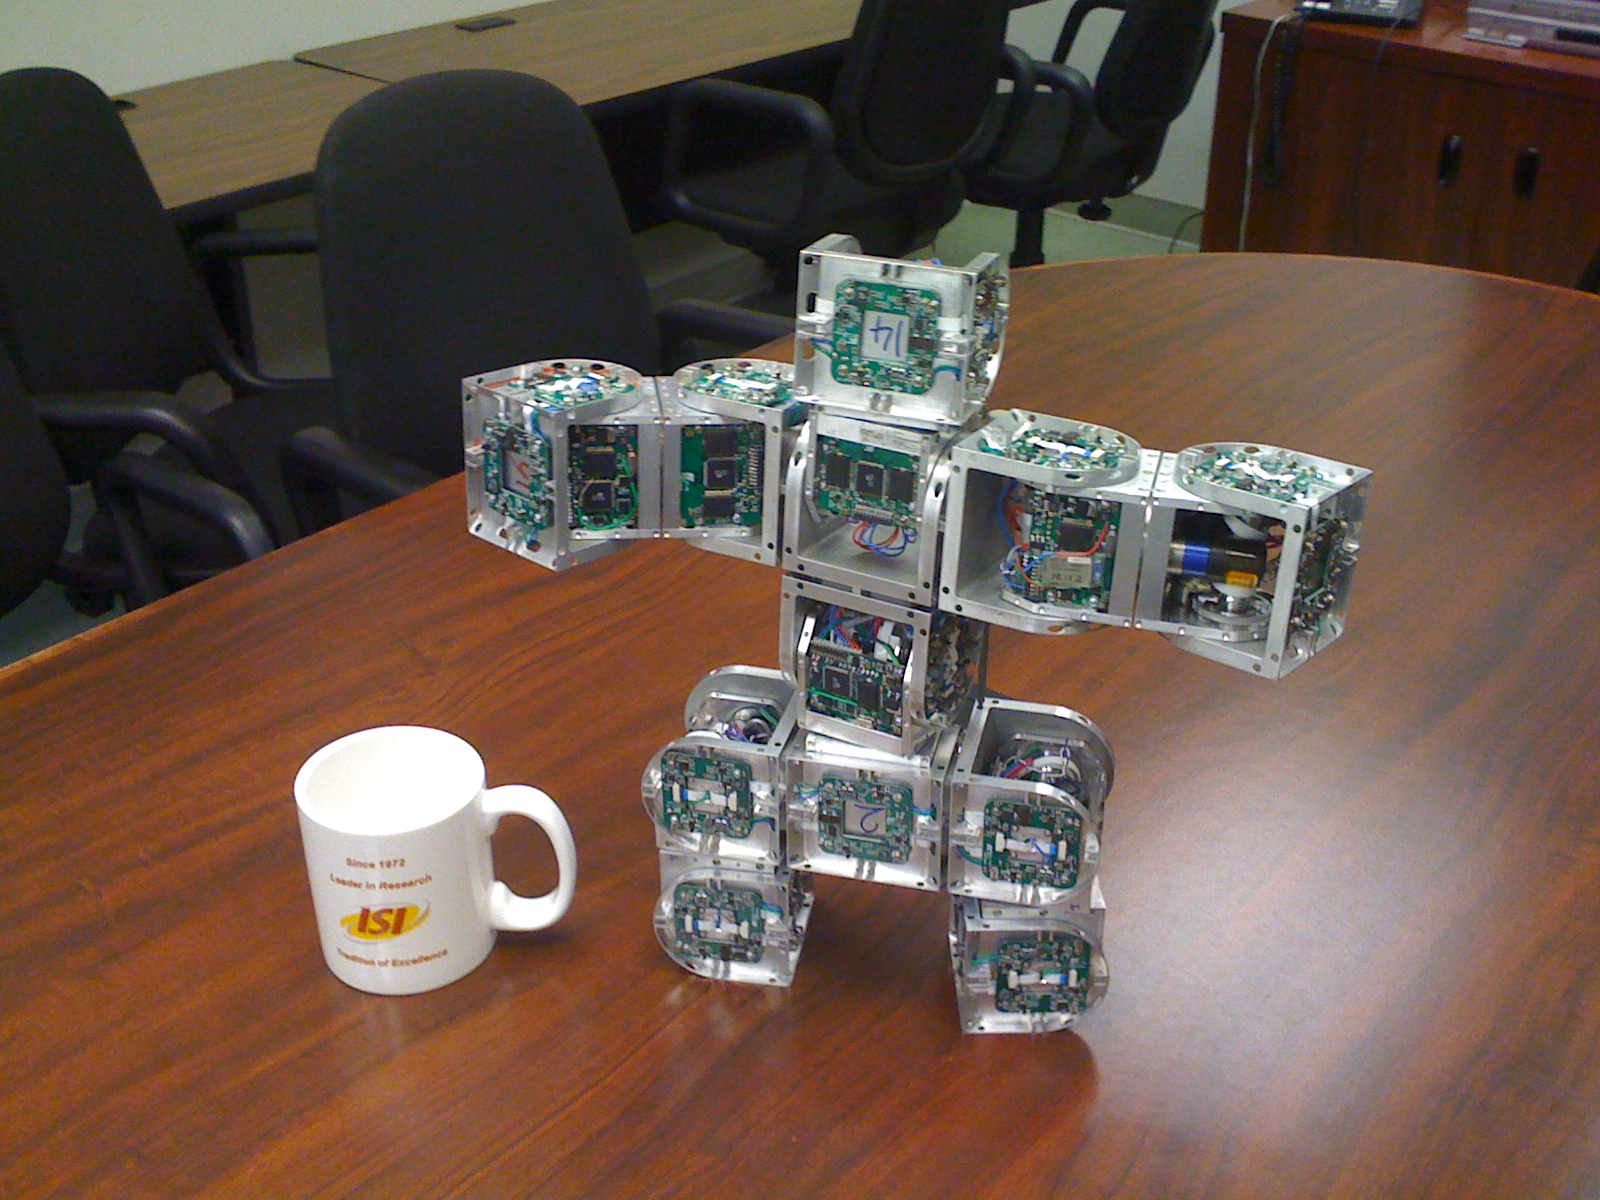
\includegraphics[height=40mm]{./fig/intro/modularrobot/SuperBotCup.jpeg}
    %     \caption{Superbot the modular robot. \cite{Superbot}}
    %     \label{superbot}
    % \end{subfigure}
    % \hfill
    \begin{subfigure}{1.0\textwidth}
        \centering
        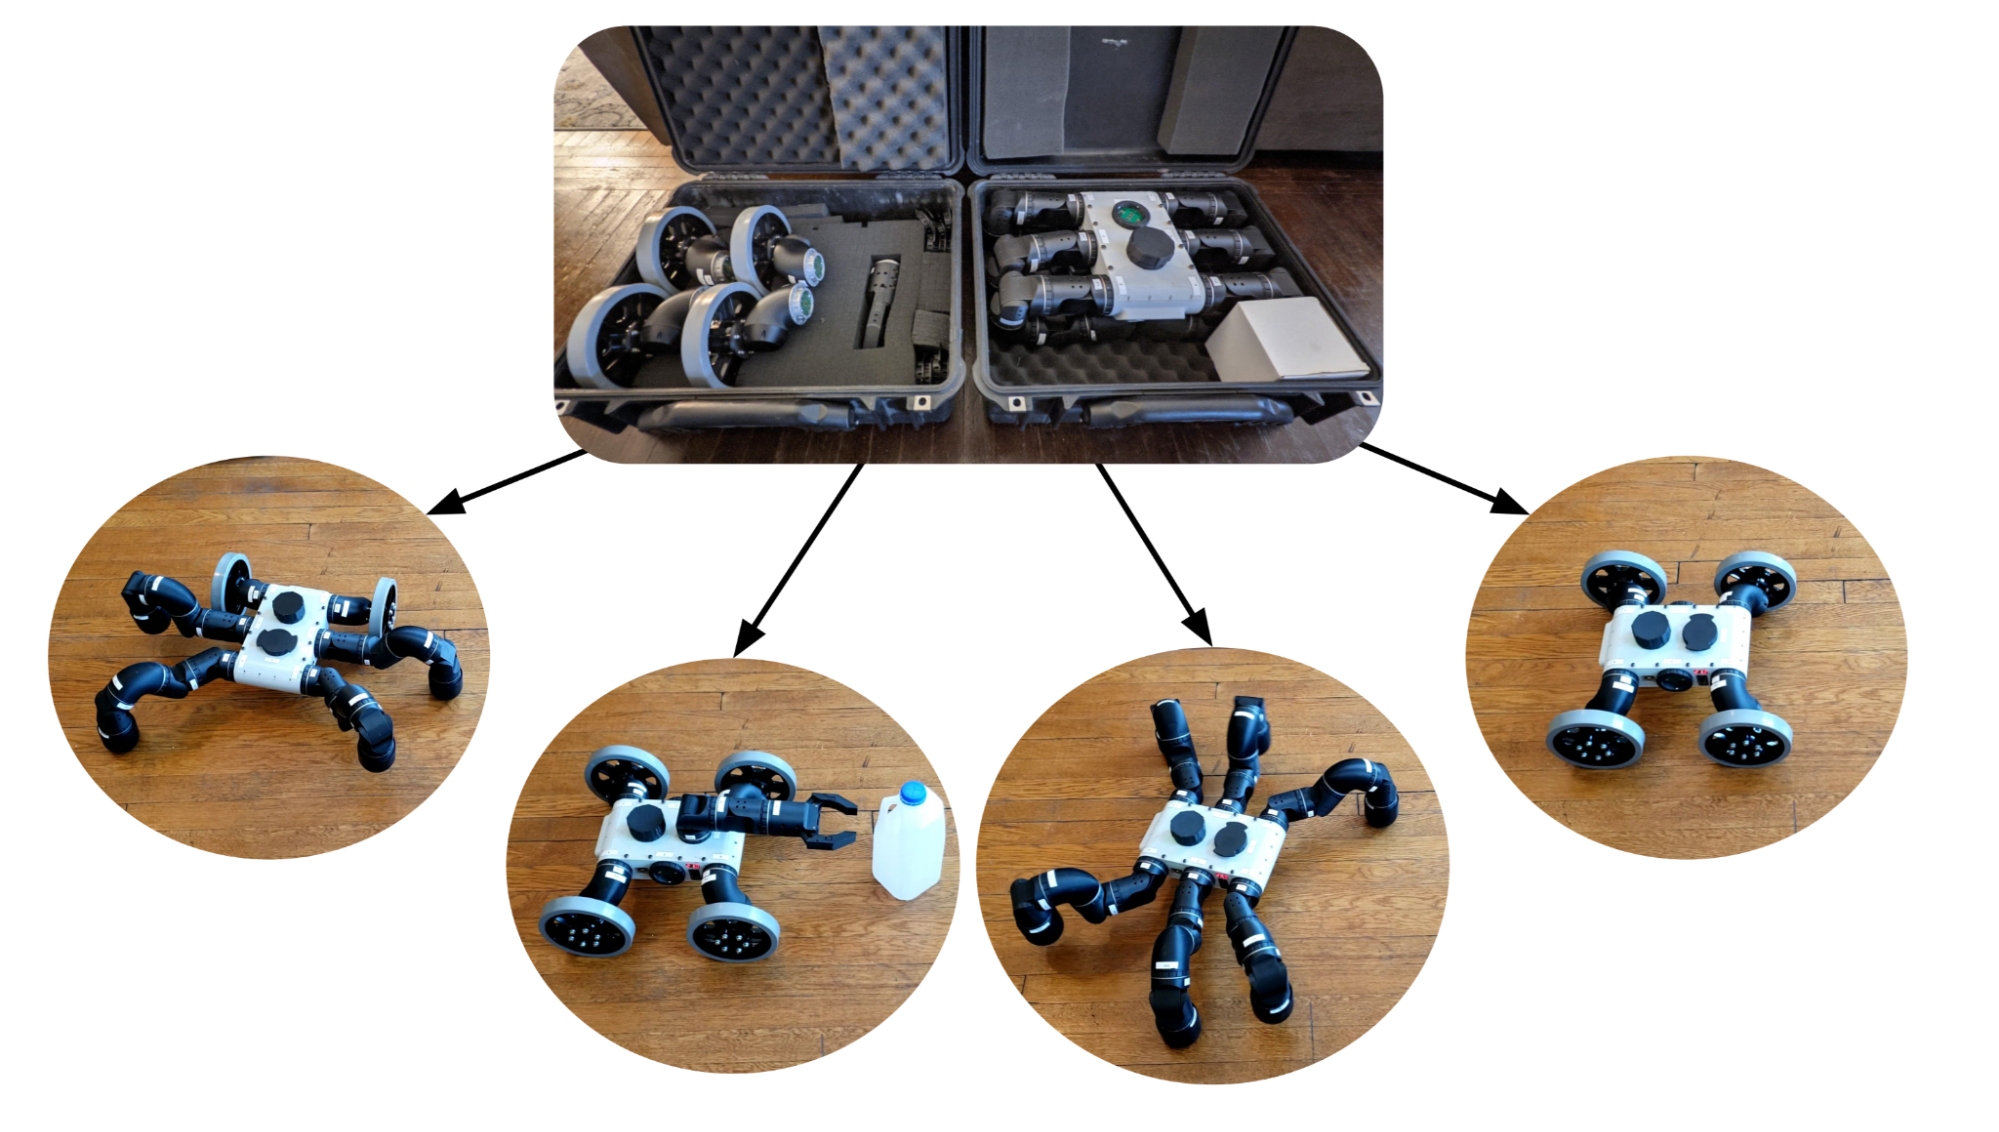
\includegraphics[height=52mm]{./fig/intro/modularrobot/Eigenbot.png}
        \caption{Superbot’s modular units self-assemble. \cite{Eigenbot}}
        \label{Eigenbot}
    \end{subfigure}
    \begin{subfigure}{0.45\textwidth}
        \centering
        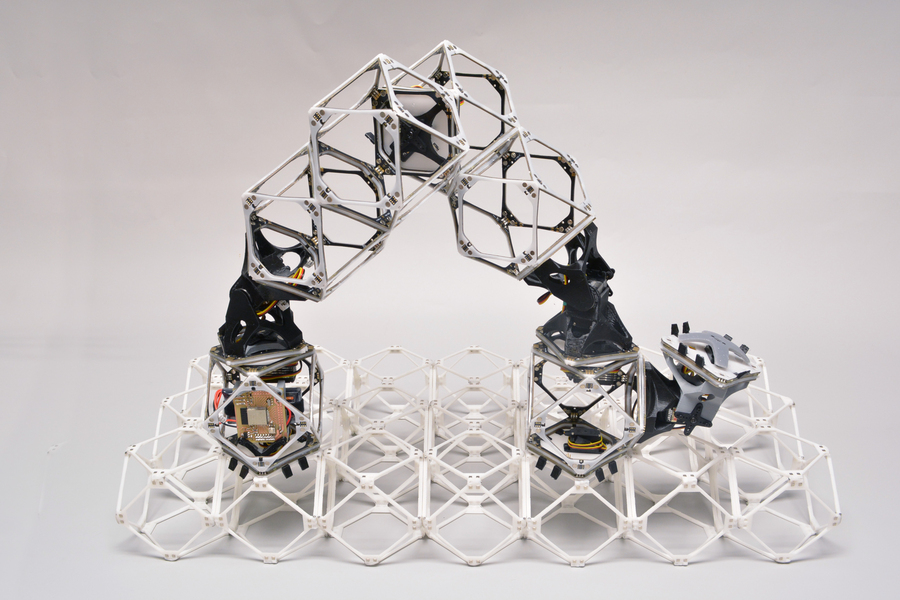
\includegraphics[height=52mm]{./fig/intro/modularrobot/MIT-Robot.jpg}
        \caption{Assembler bot from MIT. \cite{MITassembler}}
        \label{MITbot}
    \end{subfigure}
    \hfill
    \begin{subfigure}{0.45\textwidth}
        \centering
        \includegraphics[height=52mm]{./fig/intro/modularrobot/snap-bot.jpg}
        \caption{Snapbot the modular legged robot. \cite{snapbot1}}
        \label{snapbot}
    \end{subfigure}
    \vspace{2mm}
    \caption{Examples of modular robots.}
    \label{modular-robot}
\end{figure}


%%%%% Modular Robot %%%%%

%%%%% MOONSHOT PROJECT %%%%%
\section{Moonshot Project}
The Moonshot project of the Space Robotics Laboratory, led by Prof. Kazuya Yoshida at Tohoku University, aims to accomplish Goal 3: ``Realization of AI robots that autonomously learn, adapt to their environment, evolve in intelligence, and act alongside human beings by 2050" \cite{moonshotproject}. In alignment with this goal, the project envisions the development of a ``Self-evolving AI Robot System for Lunar Exploration and Human Outpost Construction"\cite{moonshotGoal3B}. The project has identified several key objectives to achieve this vision:
\vspace{1mm}
\begin{enumerate}
    \item Design modular and reconfigurable heterogeneous robotic systems.
    \item Develop a transferable AI system for plug-and-play implementation.
    \item Enable on-demand robot design and on-site assembling capabilities.
\end{enumerate}

As part of the Moonshot project, our team has developed ``Moonbot", a modular robot designed to address the challenges of lunar exploration. Moonbot inherits the vision of the Moonshot project, integrating autonomous learning, adaptability, and intelligence. This modular robot represents a pioneering step towards the project's overarching goal.

Moonbot draws inspiration from innovative modularity concepts in legged robotics, including the Snapbot project \cite{snapbot1} \cite{snapbot2}, as well as general modular robotics advancements \cite{modularrobot}. These projects laid the foundation for Moonbot's approach to modularity.

The advancement of Moonbot's design is the integration of modularity concept with a higher-level legged robot control system \cite{syropod}. This combination results in a robotic platform capable of self-recognition, adaptability, and dynamic selection of control motions. Moonbot inherits the ability to configure its legs dynamically, ranging from one to four, thus enhancing its versatility and locomotion capabilities.\\

\begin{figure}[t]
  \centering
  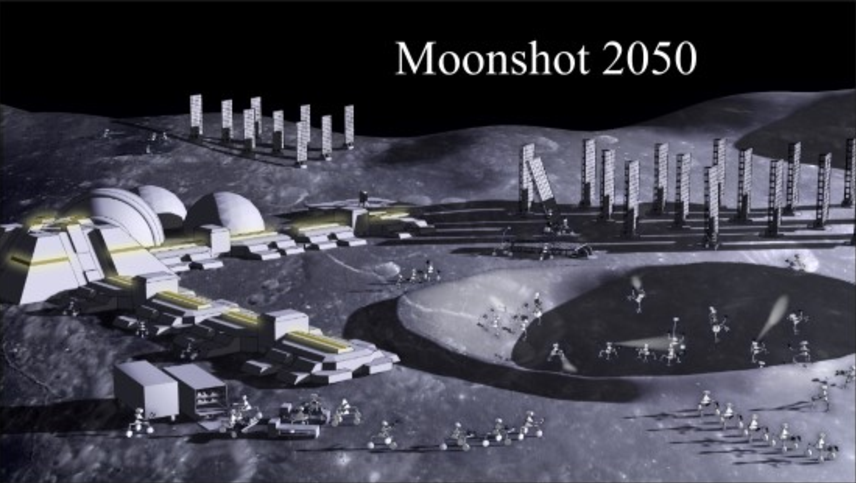
\includegraphics[width=\linewidth]{./fig/intro/moonshot.pdf}
  \vspace{2mm}
  \caption{lunar base with AI robots in 2050. \cite{moonshotGoal3B}}\label{fig moonshot}
\end{figure}
%%%%% MOONSHOT PROJECT %%%%%

%%%%% OBJ %%%%%
\section{Research Objectives}
This thesis aims to develop the first prototype of modular control system for legged robots. By using the implemented internal sensors, the robot can recognize the configuration and select the appropriate strategy of motion control, referred as self-recognition ability.

Secondly, the research aims to realize sophisticated software control mechanisms and high-level controllers for the quadruped modular robot. By designing and implementing robust software architectures, the robot can execute complex locomotion patterns. Through these objectives, the research endeavors to enhance the autonomy, adaptability, and overall performance of modular legged robots, paving the way for advancements in robotic exploration and deployment scenarios.\\
%%%%% OBJ %%%%%

% \section{Research Plan Proposal}
% The email address below is the author's contact information. We are always accepting bug reports and questions. \\
% \texttt{unoken@tohoku.ac.jp}

%%%%% OVERVIEW %%%%%
\section{Thesis Overview}
The structure of this thesis is outlined below. 

\begin{itemize}
    \item \textbf{Chapter 1: Introduction}: \\
    This chapter serves as an introduction to the thesis, providing background information and the purpose behind the research.
   
    \item \textbf{Chapter 2: Modular Legged Robot: "Moonbot"}: \\
    This chapter offers an in-depth exploration of Moonbot's structural composition, focusing on its hardware overview, modularity, and self-recognition capabilities.

    \item \textbf{Chapter 3: Software and Self-Recognition Algorithms}: \\
    Here, the thesis delves into the software architecture and logic of Moonbot's self-recognition algorithms, detailing the tools and methodologies used in their development.

    \item \textbf{Chapter 4: Motion Control}: \\
    This chapter examines Moonbot's motion control mechanisms, including its kinematics and locomotion strategies. It provides insights into how the robot navigates and moves within its environment.

    \item \textbf{Chapter 5: Conclusions}: \\
    The final chapter concludes the thesis with a summary of the achieved results, reflections on the challenges encountered, and proposals for future advancements in lunar exploration robotics.
\end{itemize}

%%%%% OVERVIEW %%%%%

%%% EOF %%%

\chapter{Modular Legged Robot:``Moonbot"}
%\label{cha:AAAA}
%%%%%%%%%%%%%%%%%%%%%%%%%%%%%%%%%%%%%%%%%%%%%%%%%%%%%%%%%
%%%
%%%  Chapter 2
%%%  Robot Overview
%%%
%%%%%%%%%%%%%%%%%%%%%%%%%%%%%%%%%%%%%%%%%%%%%%%%%%%%%%%%%
Moonbot is the first version of a modular robot model for the Moonshot project, "Self Evolving AI Robot System for Lunar Exploration and Human Outpost Construction". The aimed technologies of this robot are self-reconfigurable and self-assembly abilities. 

Using the internal sensors between main body and modular legs, Moonbot autonomously performs a real-time self-recognition system to identify the locomotion style fitting with the configuration.\\

\begin{figure}[ht]
  \centering
  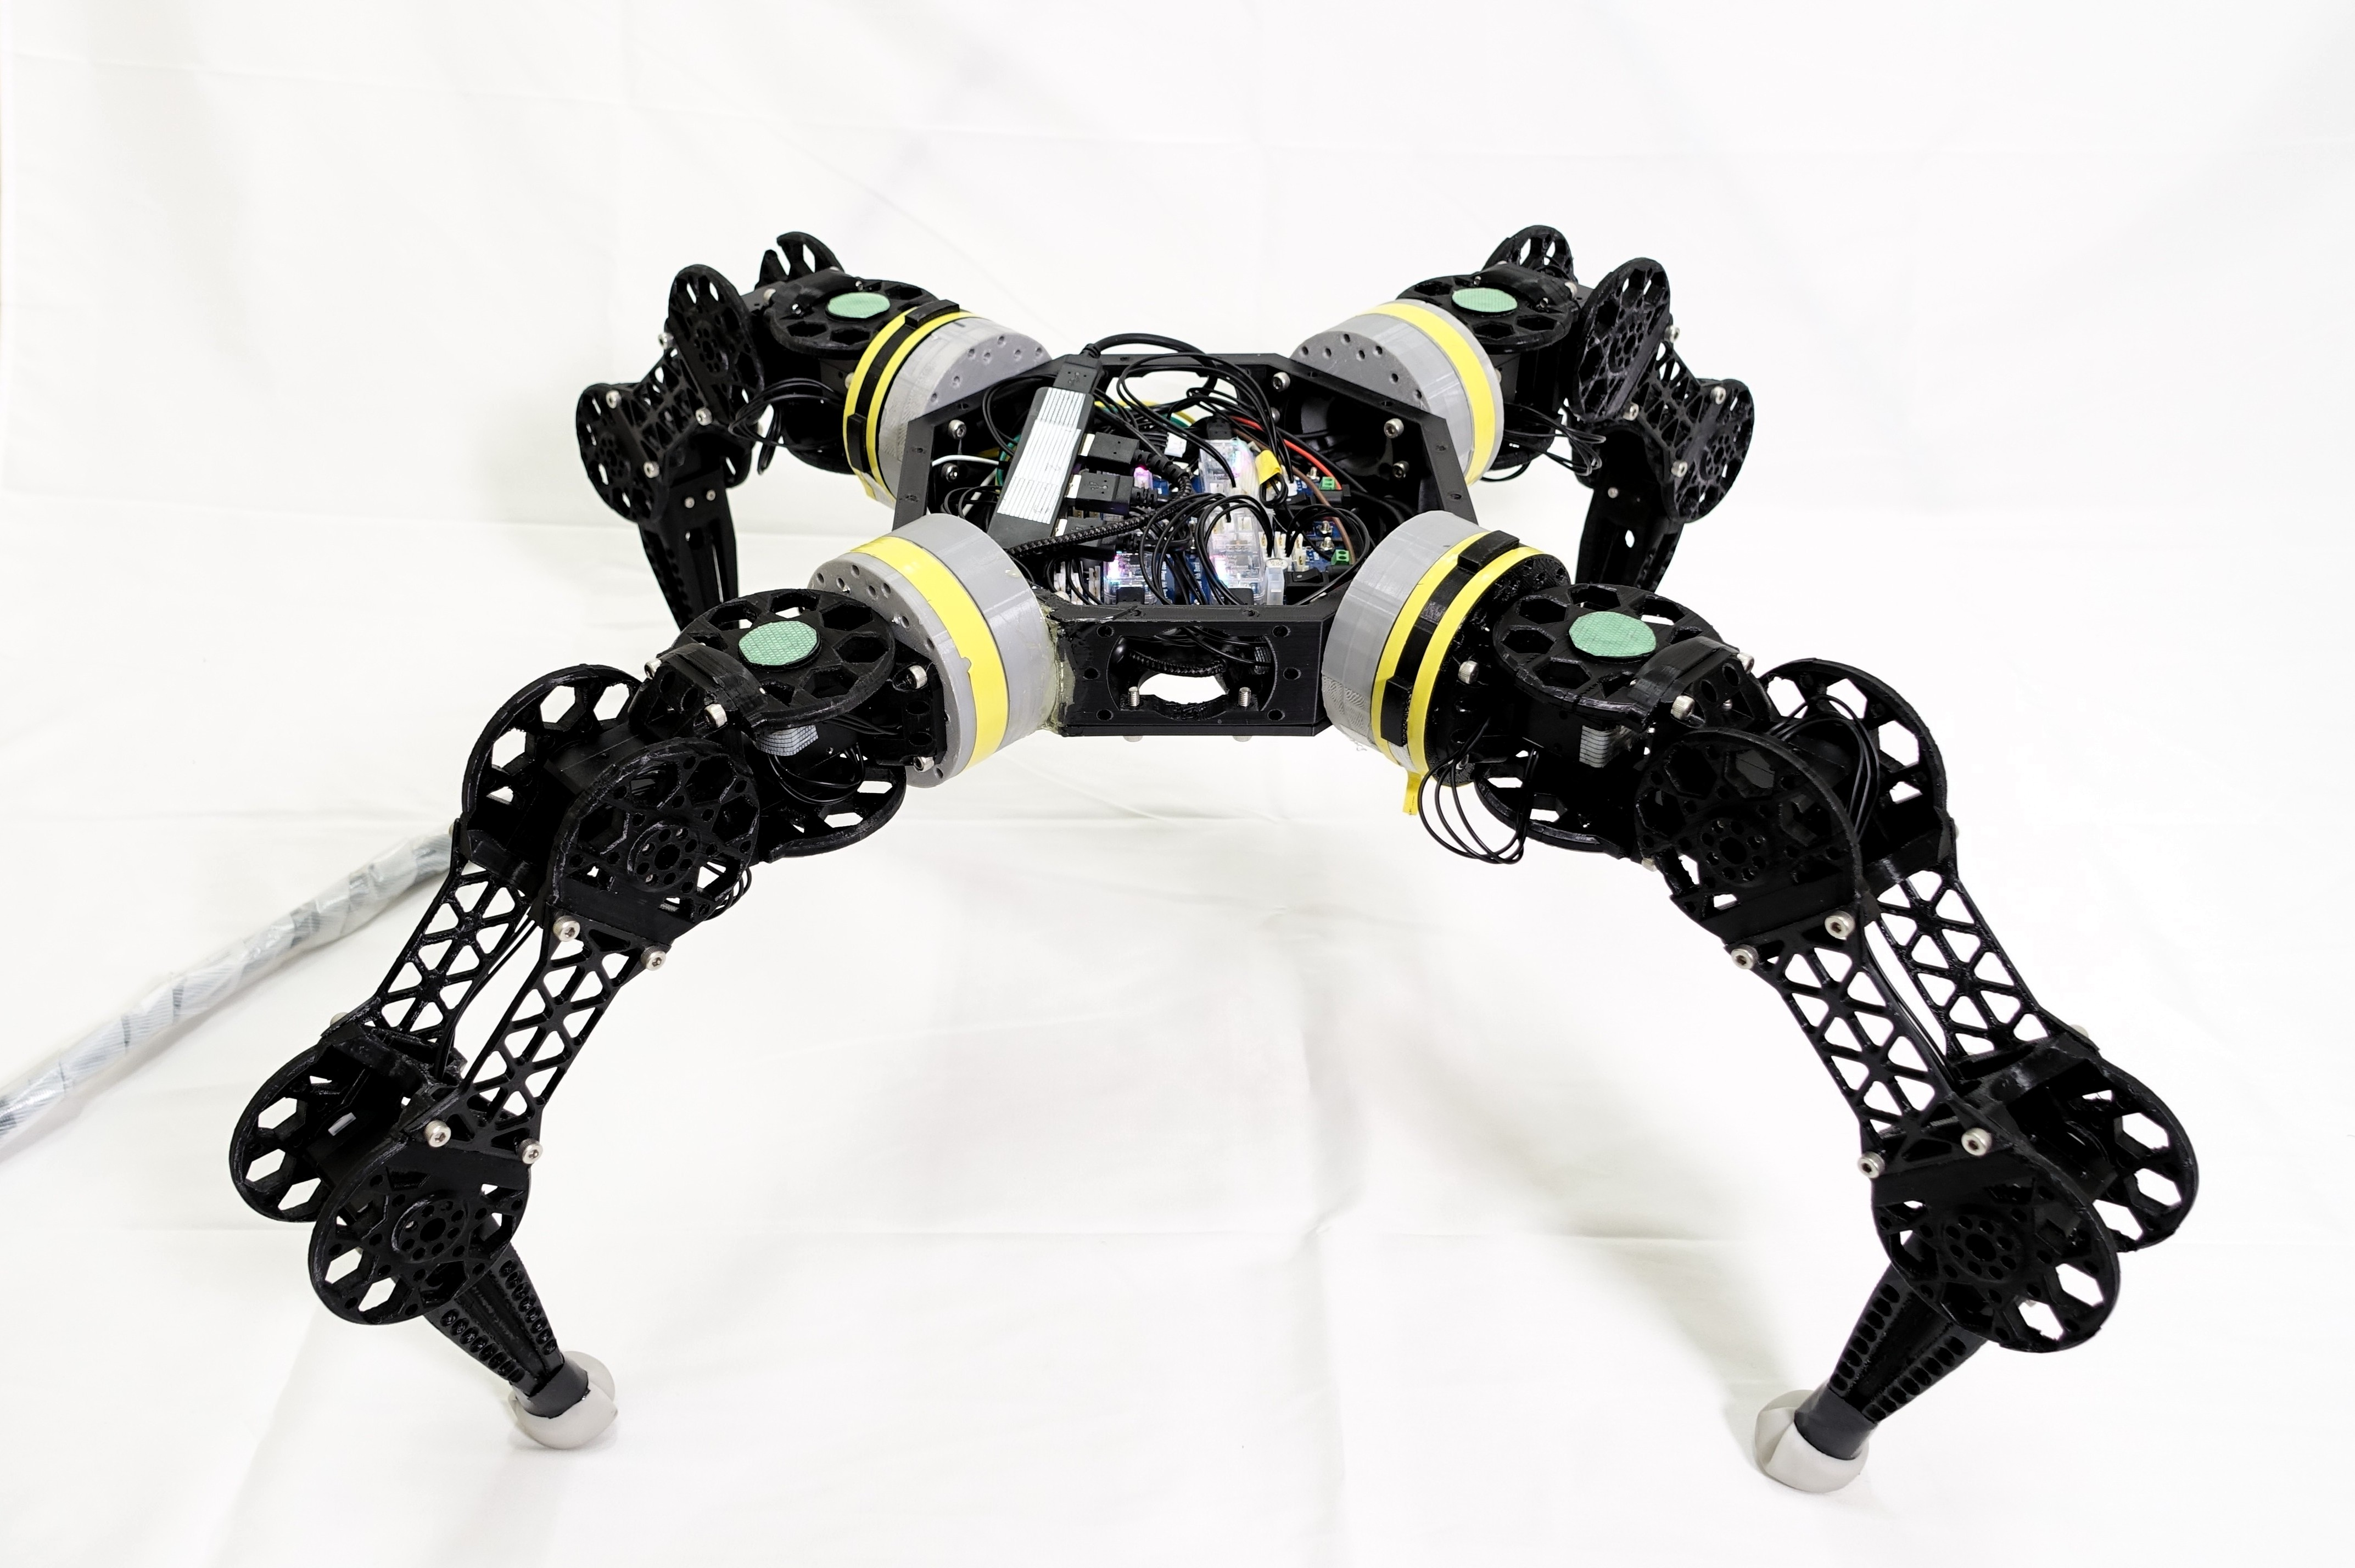
\includegraphics[width=100mm]{./fig/moonbot/moonbot1.jpg}
  \vspace{2mm}
  \caption{Moonbot with full configuration on the sand box.}\label{fig moonbot}
\end{figure}

%%%%% HARDWARE DESIGN %%%%%
\section{Hardware Design} % Find the exact material and add citation
The Moonbot's parts are mainly made of PLA (Ploylactic Acid) \cite{PLA}, 3D printed. The  Moonbot's components consist of central body and four leg modules. The legs are connected via magnetic connection. The communications of each leg and the computer transfer via pogo pin connector. In the this section, the mechanical design and electronic of Moonbot are explained

\subsection{Central Body}
The Moonbot's central body is 20x20 cm square shape. The total weight, including all electronic components, is 1.02 kilograms. On the body, there are four U2D2 and U2D2 hub, a USB communication converter for connecting with servo motors. This converter is available for various communication protocol, including 4-pin UART, 3-pin TTL, and 4-pin RS-485. In this time, 3-pin TTL is selected. At the bottom of the body, four ball casters are attached to support the locomotion style where the body of the robot lies on the floor. At each corner of the shape, four ports of magnetic connection are anchored.\\

\begin{figure}[t]
  \centering
  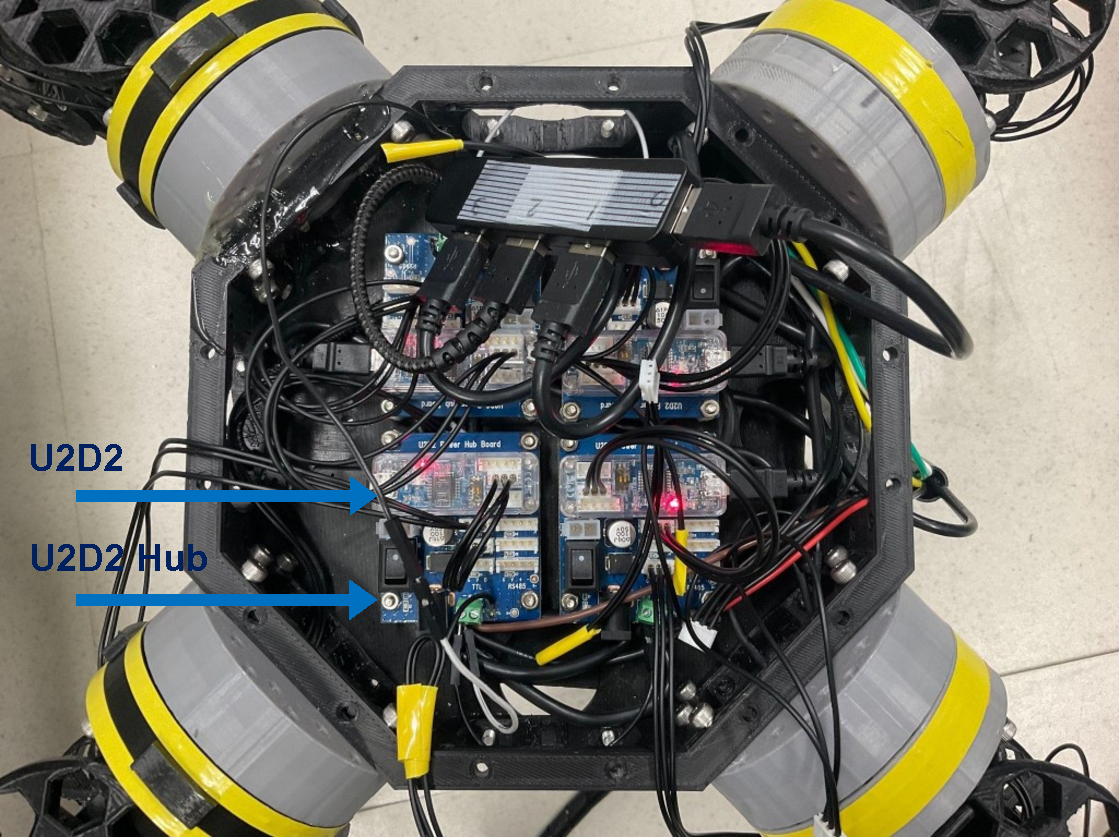
\includegraphics[width=90mm]{./fig/chap2/bodyelectronics.pdf}
  \vspace{2mm}
  \caption{Electronics components on the Moonbot center hub.}\label{electronics}
\end{figure}

\begin{figure}[t]
  \centering
  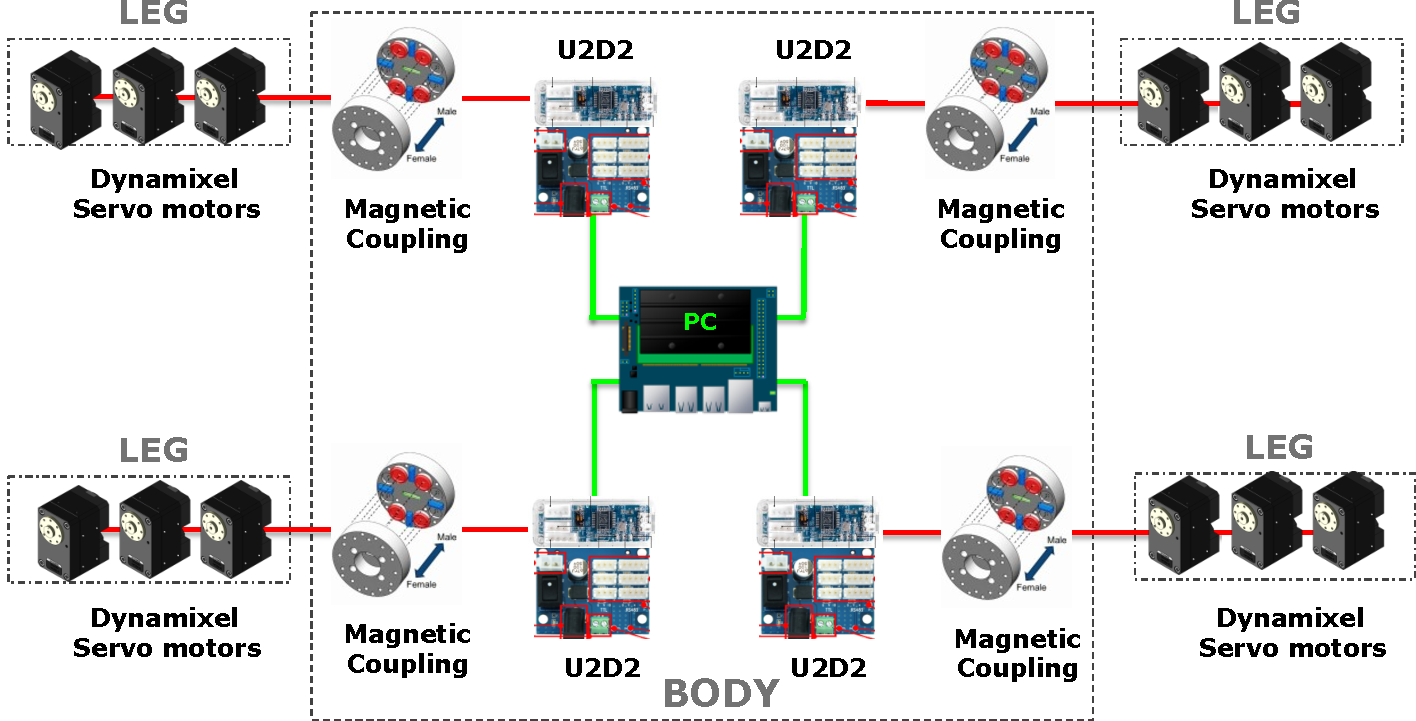
\includegraphics[width=140mm]{./fig/chap2/electronics_diagram.pdf}
  \vspace{2mm}
  \caption{Electronics components on the Moonbot center hub.}\label{electronics_diagram}
\end{figure}

\subsection{Magnetic Coupling}
Each of the legs is connected to the body via 8 pairs of circular Neodynium magnets, arranged in circular pattern as shown in as shown in \fig{magnet}. A piese of magnet has 180 grams of weight, 3 mm in height and 150 mm of diameter.

\begin{figure}[t]
  \centering
  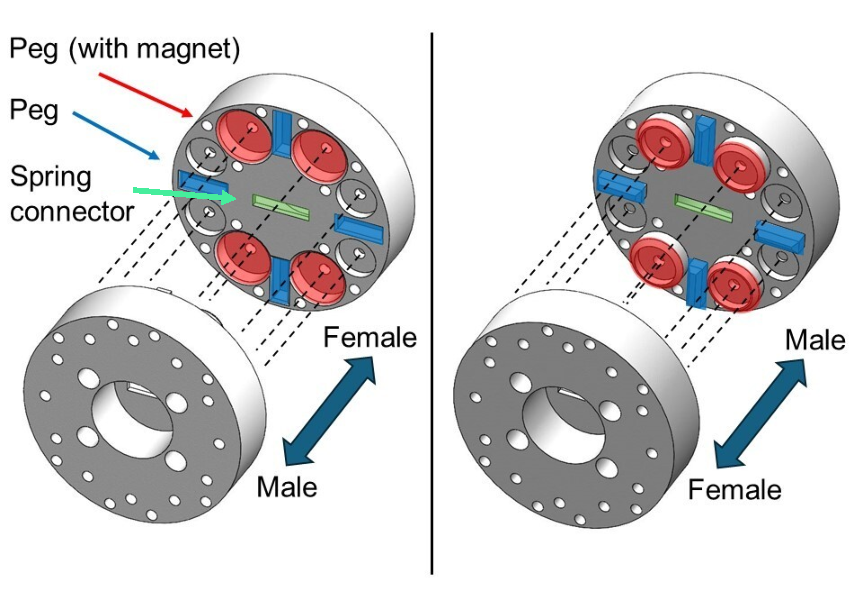
\includegraphics[width=110mm]{./fig/chap2/pogopin/connector2.pdf}
  \vspace{2mm}
  \caption{Magnetic connector.}\label{magnet}
\end{figure}

In addition to the magnetic coupling, the electronics connections between the body and the legs are facilitated by pogo pins. Pogo pins, also known as spring-loaded pins, provide a reliable electrical connection between two components while allowing for movement and flexibility. This spring loaded connector is attached at the center of the magnetics connector of each module as shown in \fig{pogopin}\\

\begin{figure}[h]
  \centering
  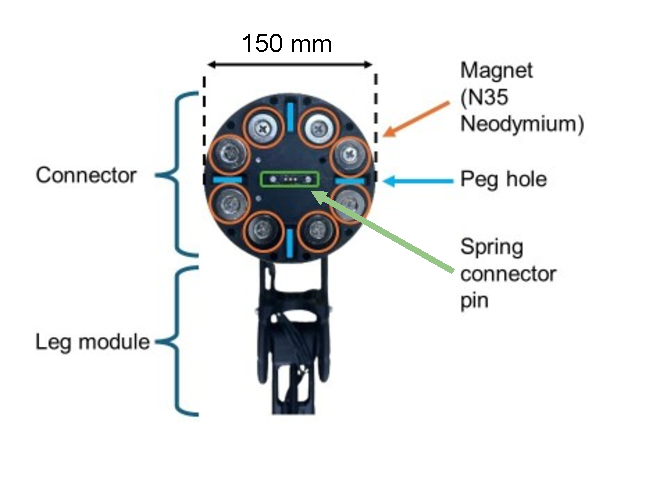
\includegraphics[width=120mm]{./fig/chap2/pogopin/connector.pdf}
  \vspace{2mm}
  \caption{Pogo pin connector located at the middle of magnetic coupling.}\label{pogopin}
\end{figure}

% \begin{figure}[t]
%     \begin{subfigure}{1.0\textwidth}
%      \begin{center}
%       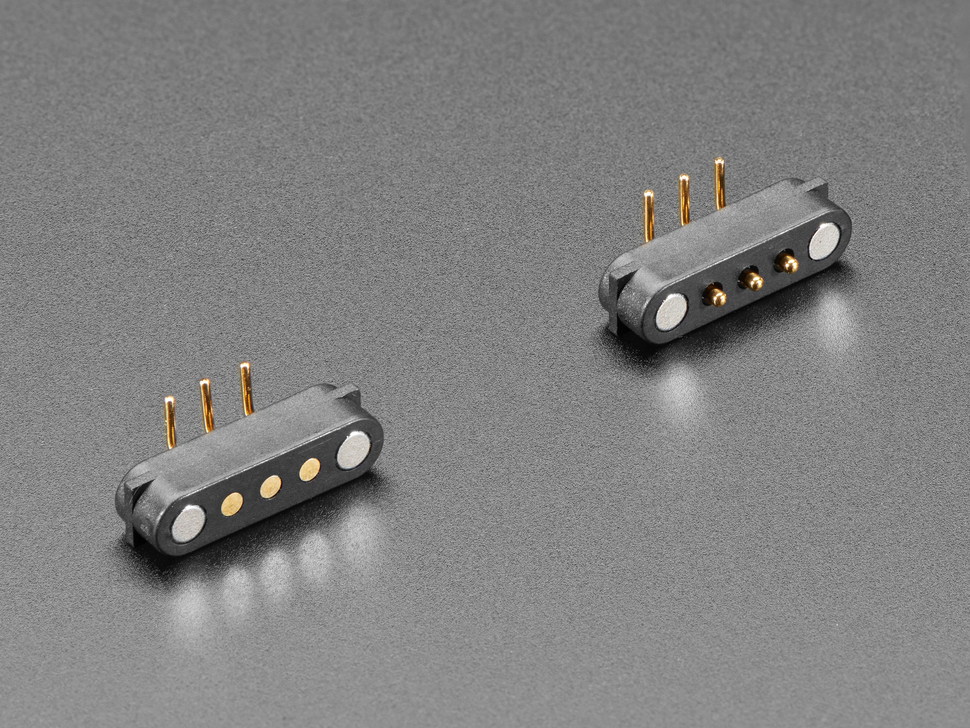
\includegraphics[height=30mm]{./fig/chap2/pogopin/pogopin3pin.jpg}
%     \caption{Three contact pins connector}\label{pogopin1}
%      \end{center}
%     \end{subfigure}
    
%     \begin{subfigure}{1.0\textwidth}
%      \begin{center}
%       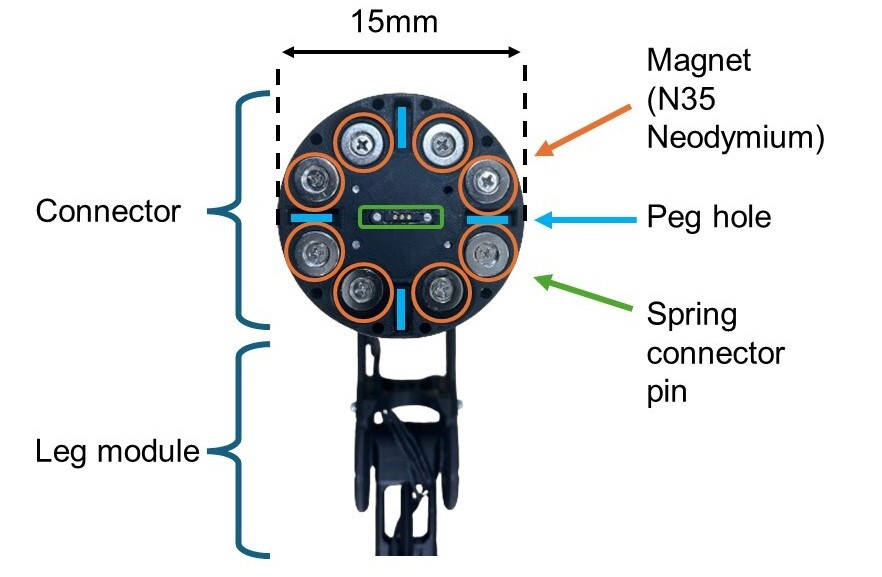
\includegraphics[height=70mm]{./fig/chap2/pogopin/connector.jpg}
%     \caption{Pogopin of the leg module}\label{pogopin2}
%     \end{center}
%     \end{subfigure}
%     \vspace{2mm}
%     \caption{Overview of magnet-based connector}
%     \label{pogopin}
% \end{figure}

\subsection{Modular Leg Modules}
Moonbot consists of four modular legs, utilizing a yaw-pitch-pitch configuration. Each of the leg has 530 grams with a small cylindrical end effector.The lengths of each link of the leg are shown in Table \ref{moonbot params}

\vspace{\baselineskip}
\begin{table}[h]
  \centering
    \caption{Moonbot's leg parameters.}
     \begin{tabular}{rrr} 
     \bhline{1.2pt}
      \multicolumn{1}{c}{Link's name}&\multicolumn{1}{c}{Length [mm]} \\
      % \multicolumn{1}{c}{of data}&\multicolumn{1}{c}{[mm]}&\multicolumn{1}{c}{±std [mm] } \\
      \hline
      Coxa	&	64.55		\\
      Femur	&	129.0	\\
      Tibia	&	156.0	\\
     \bhline{1.2pt}
    \end{tabular}
    \vspace{2mm}
    \label{moonbot params}
\end{table}
% \vspace{\baselineskip}

\begin{figure}[h]
  \centering
  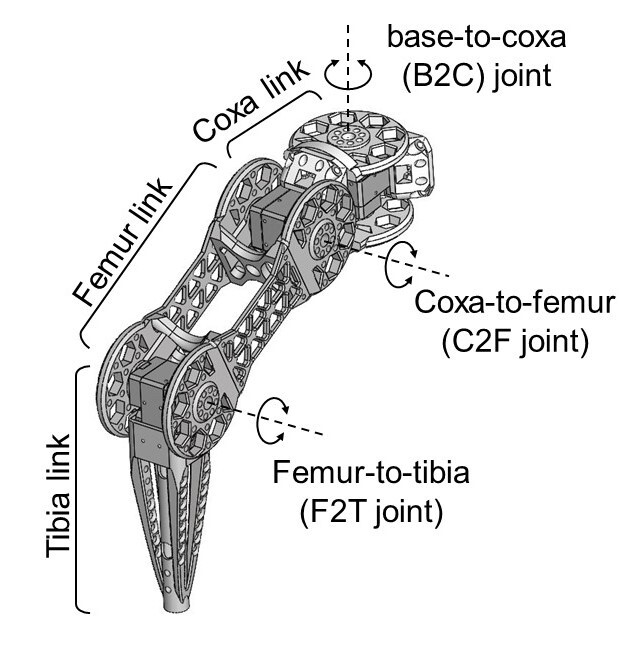
\includegraphics[width=90mm]{./fig/leg_configuration/CAD.jpg}
  \vspace{2mm}
  \caption{Moonbot's modular legs.}\label{modules}
\end{figure}

%%%%% SERVO %%%%%
\subsection{Joints' Actuator: Dynamixel}
Dynamixel is a brand of high-performance smart servos developed by ROBOTIS~\cite{robotis}. These servos are widely used in robotics applications due to their precision, durability, and advanced features. Dynamixel servos are known for their ability to provide position, velocity, and torque control, as well as various feedback mechanisms.

The joints of the Moonbot is moved by Dynamixel XM430-350-T, utilizing a 3-pin TTL communication protocol, Moonbot can generate trajectories with precise position control. The specification of this servo is shown below\\

\begin{figure}[t]
  \centering
  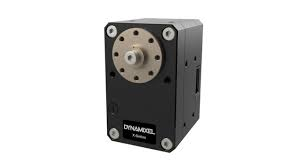
\includegraphics[width=90mm]{./fig/chap2/dxl.jpeg}
  \vspace{2mm}
  \caption{Dynamixel servo motor, model XM430-W350-T.}\label{DXL}
\end{figure}
\smallskip
\begin{table}[t]
    \centering
    \caption{Dynamixel XM430-W350-T Specifications.}
    \label{dynamixel_spec}
    \begin{tabular}{|l|l|}
        \hline
        \rowcolor[HTML]{EFEFEF}
        \multicolumn{2}{|c|}{\cellcolor[HTML]{EFEFEF}\textbf{Specifications}} \\ \hline
        \textbf{Parameter} & \textbf{Value} \\ \hline
        Speed & 46 RPM \\ \hline
        Torque & 4.1 N$\cdot$m  \\ \hline
        Size & 33.5$\times$46.5$\times$34.0 mm \\ \hline
        Mass & 82 g \\ \hline
    \end{tabular}
\end{table}
\smallskip
%%%%% SERVO %%%%%

%%%%% HARDWARE DESIGN %%%%%
%%% EOF %%%

\chapter{Software and Self-Recognition Algorithms}
%\label{cha:BBBB}
%%%%%%%%%%%%%%%%%%%%%%%%%%%%%%%%%%%%%%%%%%%%%%%%%%%%%%%%%
%%%
%%%  第3章
%%%  図表等の挿入
%%%
%%%%%%%%%%%%%%%%%%%%%%%%%%%%%%%%%%%%%%%%%%%%%%%%%%%%%%%%%
Moonbot, designed for lunar surface operations, relies on a sophisticated software foundation. This chapter describe the structure of Moonbot's software architecture and the used tools.

%%%%% ROS2 %%%%%
\section{Software Tools}
\subsection{ROS and ROS2}
\textbf{ROS (Robot Operating System):} \cite{ros} is a flexible framework for writing robot software. ROS provides services for hardware abstraction, device drivers, communication between processes, package management, and more. ROS has been widely adopted in the robotics community, fostering collaboration and the sharing of libraries and tools.

\textbf{ROS2 (Robot Operating System 2):} The next generation of ROS, ROS2 \cite{ros2} is designed to address limitations and capitalize on the lessons learned from the widespread use of its predecessor. One of the significant improvements in ROS2 is its enhanced support for the Data Distribution Service (DDS) middleware \cite{DDS}. DDS is a standardized communication middleware that facilitates efficient and reliable data exchange between distributed systems. 

By the above information, Moonbot utilizes ROS2, Foxy distribution, as the primary tool for organizing communication among its modular components. The decision to use ROS2 is motivated by its enhanced features, including:

\begin{itemize}
\item \textbf{Real-Time Capabilities:} ROS2 provides improved support for real-time systems, crucial for dynamic and responsive control.
\item \textbf{Communication Middleware:} ROS2 offers a communication middleware options, allowing components to exchange information in a distributed system.
\item \textbf{Modularity and Extensibility:} The modular and extendable structure allow developer to debug or extend the feature of the program easily.
\end{itemize}
%%%

\subsection{ROS2 Core Concepts and Elements}
\subsubsection{ROS2 Graph}
In ROS. it provide a communication network called  ``ROS graph". ROS2 process all data and connect them simultaneously via ROS2 graph. Develop utilize this concept to map the ROS2 elements to execute the program.\\

\begin{figure}[h]
  \centering
  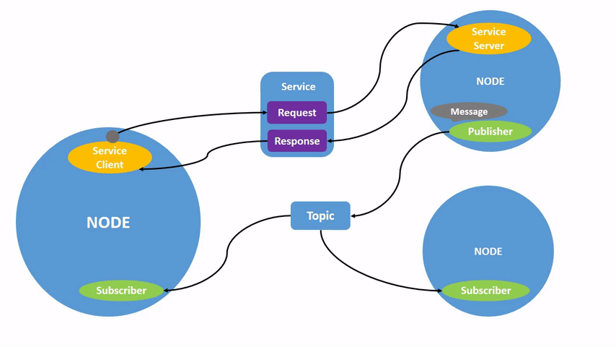
\includegraphics[width=120mm]{./fig/chap3/node.png}
  \vspace{2mm}
  \caption{Visualization of ROS2 graph. \cite{ros2}}\label{ros2_graph}
\end{figure}

\subsubsection{ROS2 Nodes}
Nodes are individual processes in a ROS 2 system. They communicate with each other by publishing and subscribing to topics, providing and using services, and executing actions.

\subsubsection{ROS2 Topics}
Topics are named buses over which nodes can exchange messages. A node can publish messages to a topic, and any other node can subscribe to that topic to receive those messages. Topics facilitate asynchronous communication between nodes.
 
\subsubsection{ROS2 Services}
Services allow request-response communication between nodes. A node provides a service by specifying a request message type and a response message type. Other nodes can then call that service by sending a request message and receiving a response message.
 
\subsubsection{ROS2 Actions}
Actions provide a way for nodes to execute long-running tasks in a goal-oriented manner. Actions consist of a goal, feedback, and result, allowing for more complex interaction patterns than services. Nodes can send action goals, receive feedback on the progress of those goals, and eventually receive a result once the goal is completed.\\
%%%%% ROS2 %%%%%

%%%%% ROS2 CONTROL %%%%%
\subsection{ROS2 Control}
Moonbot's control architecture is developed with ROS2, and within this framework, the ROS2 control package \cite{ros2control} plays a key role. In this section, we are going to delve into the specifics of ROS2 control, its integration with Moonbot's control system, and the key components that contribute to Moonbot's adaptability and precision.

\begin{figure}[ht]
  \centering
  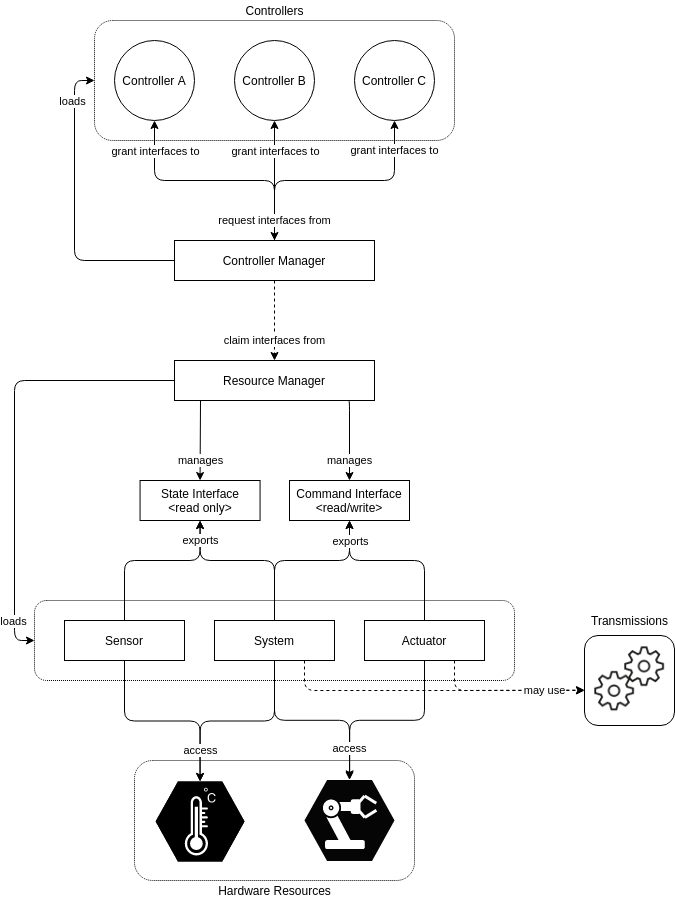
\includegraphics[width=120mm]{./fig/ros2_control/components_architecture.png}
  \vspace{2mm}
  \caption{ROS2 Control Framework. \cite{ros2control}}\label{ros2_control_framework}
\end{figure}

\subsubsection{ROS2 Control Overview}
The \texttt{ros2\_control} is a package providing a modular and configurable framework for controlling robotic systems. This package is a redevelopment of ros\_control \cite{ros_control}, used in ROS.

% In ros\_control, the rigid structure of \texttt{RobotHW} class and \texttt{CombinedRobotHardware} class \cite{ros_combined_robot_hw} are used for handling with hardware. Without any coding, this structure makes it difficult to extend additional hardware and sensor. In addition, to control the hardware, \texttt{position}, \texttt{velocity}, and \texttt{effort} are allowable.

% In ros2\_control framework, the plugins of hardware are divided into \texttt{Actuator}, \texttt{Sensor}, and \texttt{System}. Moreover, the type of hardware interface is not fixed. By the combination of these components, development of multi-robot and multi-sensor are available within this framework.

The ros\_control framework relies on the \texttt{RobotHW} class as a structure to manage hardware interactions. While it provides a rigid structure for handling various hardware components like sensors and actuators, extending existing robots with additional hardware requires coding, limiting the flexibility to integrate new elements. The use of the \texttt{CombinedRobotHardware} class \cite{ros_combined_robot_hw} attempts to address this limitation, yet it may not be optimal, especially when incorporating external sensors into the system.

In contrast, the ROS2 control framework introduces a more versatile approach by defining three types of hardware: \texttt{Actuator}, \texttt{Sensor}, and \texttt{System}. Through the composition of these basic components, any robotic cell, encompassing the robot and its surrounding environment, can be described. Unlike ros\_control, ros2\_control does not enforce a fixed set of interface types, allowing flexibility in defining interfaces. This ensures compatibility with standard controllers, as standard interfaces are defined as constants in the \texttt{hardware\_interface} package. Moreover, the \texttt{ControllerManager} in ros2\_control facilitates controlled access to the hardware by managing the state of available interfaces through the \texttt{ResourceManager}. Unlike ros\_control, controllers have no direct access to hardware, and they register their interfaces with the \texttt{ControllerManager}, enhancing modularity and resource conflict resolution.

% In Moonbot, each leg functions as an independent entity with its own controller, ensuring a high degree of modularity. This design choice aligns seamlessly with the modular structure of Moonbot, allowing for efficient control and adaptability across different leg configurations.

\subsubsection{Controller Manager}
At the heart of the ROS2 control architecture lies the Controller Manager. This component is responsible for loading, managing, and switching between different controllers. In Moonbot, the Controller Manager coordinates the operation of controllers associated with each leg, allowing dynamic transitions between various locomotion styles based on the robot's configuration.

\subsubsection{ROS2 Life Cycle}
ROS2 Lifecycle \cite{ros2lifecycle} is utilized in controller manager of ROS2 control. The ROS 2 Node Lifecycle provides enhanced control over the state of the ROS system, as shown in \fig{lifecycle}, ensuring the proper initualization of all components before executing any behavior. This mechanism enables nodes to be restarted or replaced while the system is running.

A key aspect emphasized in this document is the concept of a managed node, which adheres to a predefined interface and operates within a well-defined life cycle state machine. By treating managed nodes as black boxes, developers have flexibility in implementing the life cycle functionality while ensuring compatibility with management tools across all compliant nodes.\\

\begin{figure}[t]
  \centering
  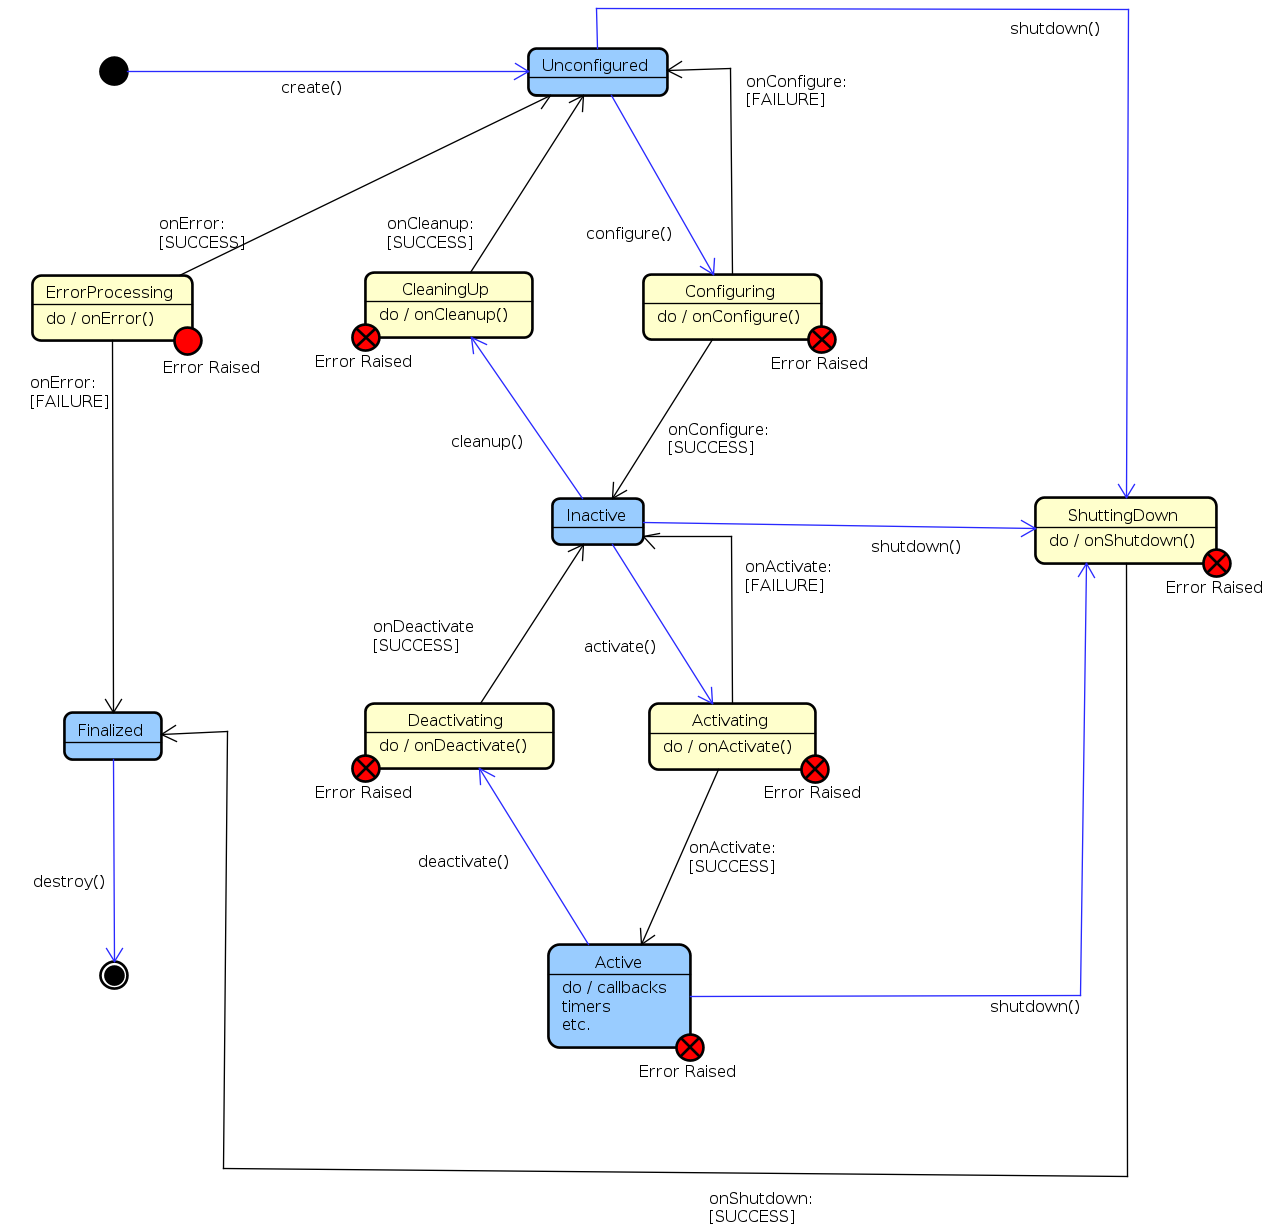
\includegraphics[width=\linewidth]{./fig/ros2_control/life_cycle_sm.png}
  \vspace{2mm}
  \caption{ROS2 Node Lifecycle. \cite{ros2lifecycle}}\label{lifecycle}
\end{figure}

\subsection{Dynamixel SDK \& Workbench}

\subsubsection{Dynamixel SDK}

The Dynamixel SDK (Software Development Kit) \cite{dynamixel-sdk} is a set of libraries and tools provided by ROBOTIS to interface with Dynamixel servos. It includes APIs (Application Programming Interfaces) for various programming languages such as C, C++, Python, and MATLAB, allowing developers to control Dynamixel servos easily from their preferred programming environment.

Key features of the Dynamixel SDK include:

\begin{itemize}
    \item \textbf{High-level APIs:} The SDK provides high-level APIs that abstract the low-level communication protocols of Dynamixel servos, making it easier for developers to control and interact with the servos.
    
    \item \textbf{Advanced control functionalities:} It offers advanced control functionalities such as position control, velocity control, torque control, and compliance control.
    
    \item \textbf{Diagnostic tools:} The SDK includes diagnostic tools that allow developers to monitor the status of Dynamixel servos, diagnose issues, and perform troubleshooting.
    
    \item \textbf{Community support:} ROBOTIS provides extensive documentation, tutorials, and forums to support developers using the Dynamixel SDK, fostering a vibrant community of users who share knowledge and resources.
\end{itemize}

\subsubsection{Dynamixel Workbench}
In addition to the Dynamixel SDK, ROBOTIS offers the Dynamixel Workbench \cite{dynamixel_workbench}, a higher-level software framework built on top of the SDK. Dynamixel Workbench provides a comprehensive set of tools and utilities for managing Dynamixel-based robotic systems. It includes features such as:

\begin{itemize}
    \item \textbf{Motion editing:} Dynamixel Workbench allows users to create and edit motion sequences for controlling Dynamixel servos in complex robotic behaviors.
    
    \item \textbf{Parameter tuning:} Users can adjust various parameters of Dynamixel servos, such as PID gains, compliance margins, and operational limits, to optimize performance and behavior.
    
    \item \textbf{Hardware interface:} Dynamixel Workbench includes APIs and drivers for interfacing with Dynamixel hardware, allowing users to communicate with servos, sensors, and other peripherals especially with ROS2 communication.
\end{itemize}

Together, the Dynamixel SDK and Dynamixel Workbench provide a powerful ecosystem for developing and controlling Dynamixel-based robotic systems, offering flexibility, scalability, and ease of use for researchers, educators, and hobbyists alike.

The Pinging function \cite{dynamixel_sdk_ping_protocol}, within Dynamixel SDK, serves as a fundamental component crucial for self-recognition algorithms in Moonbot. This function plays a pivotal role in enabling the system to identify and communicate with connected specific ID Dynamixel servos. By sending a ping command to each servo, the system can receive a response indicating the presence and status of the servos. This information is essential for initializing, configuring, and monitoring the servos within the robotic framework. 

%%%

\section{Self-Recognition}\label{HowToInsertLink}
In the context of our robotic system, self-recognition refers to the ability of the robot to autonomously assess the status and connectivity of its modules

Moonbot's adaptability is a cornerstone of its design, allowing for dynamic reconfiguration through the attachment and detachment of modules via magnetic connectors. To effectively control the robot, it is imperative for Moonbot to possess self-awareness regarding its current configuration and the type of connected module (e.g., yaw-pitch-pitch leg, gripper).

\subsection{Problem Statements}
\begin{enumerate}
    \item The robot need to be able to activate and deactivate the controller for any kinds of the module.

    \item With the different number of connected modules, the robot moves with different motion style.

\begin{figure}[h]
  \centering
  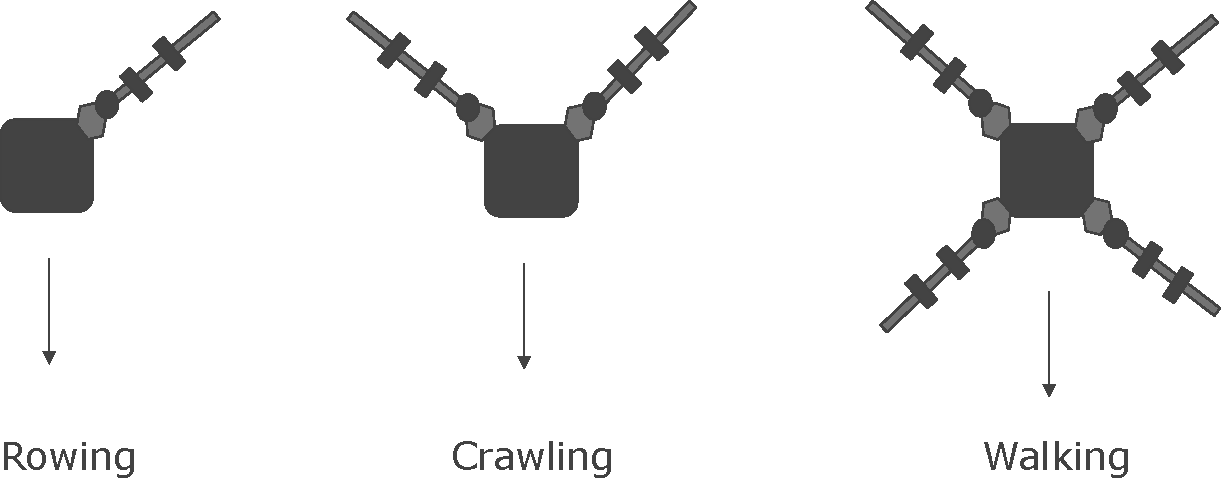
\includegraphics[width=110mm]{./fig/chap3/control_system/motion_selection.pdf}
  \vspace{2mm}
  \caption{Motion selection strategies for different number of module connections.}\label{motion_selection}
\end{figure}

    \item With the different kinds of module, the robot selects the proper motion for the specific module type.

\begin{figure}[h]
  \centering
   \rotatebox{90}{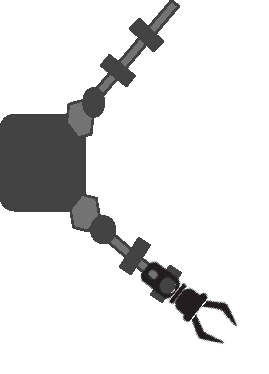
\includegraphics[width=35mm]{./fig/chap3/control_system/gripleg2.pdf}}
  \vspace{2mm}
  \caption{Different kind of modules connected to the robot.}\label{gripper}
\end{figure}
\end{enumerate}

\subsection{Algorithms Overview}
Inspired by the design of Snapbot, a modular-legged robot developed by Disney Inc. \cite{snapbot1}, \cite{snapbot2}, Moonbot employs a self-recognition system. The connections are periodically verified by pinging the specific ID of Dynamixel motors. The flowchart in \fig{flowchart} and Algorithm~\ref{alg:module_recognition} shows the modular connection algorithm for one connector. After the robot identifies the type of module, the module's controller at the specific port is independently launched, and activated. With the specific configuration identified, Moonbot then selects the appropriate locomotion style.
\vspace{1mm}

\begin{figure}[h]
  \centering
  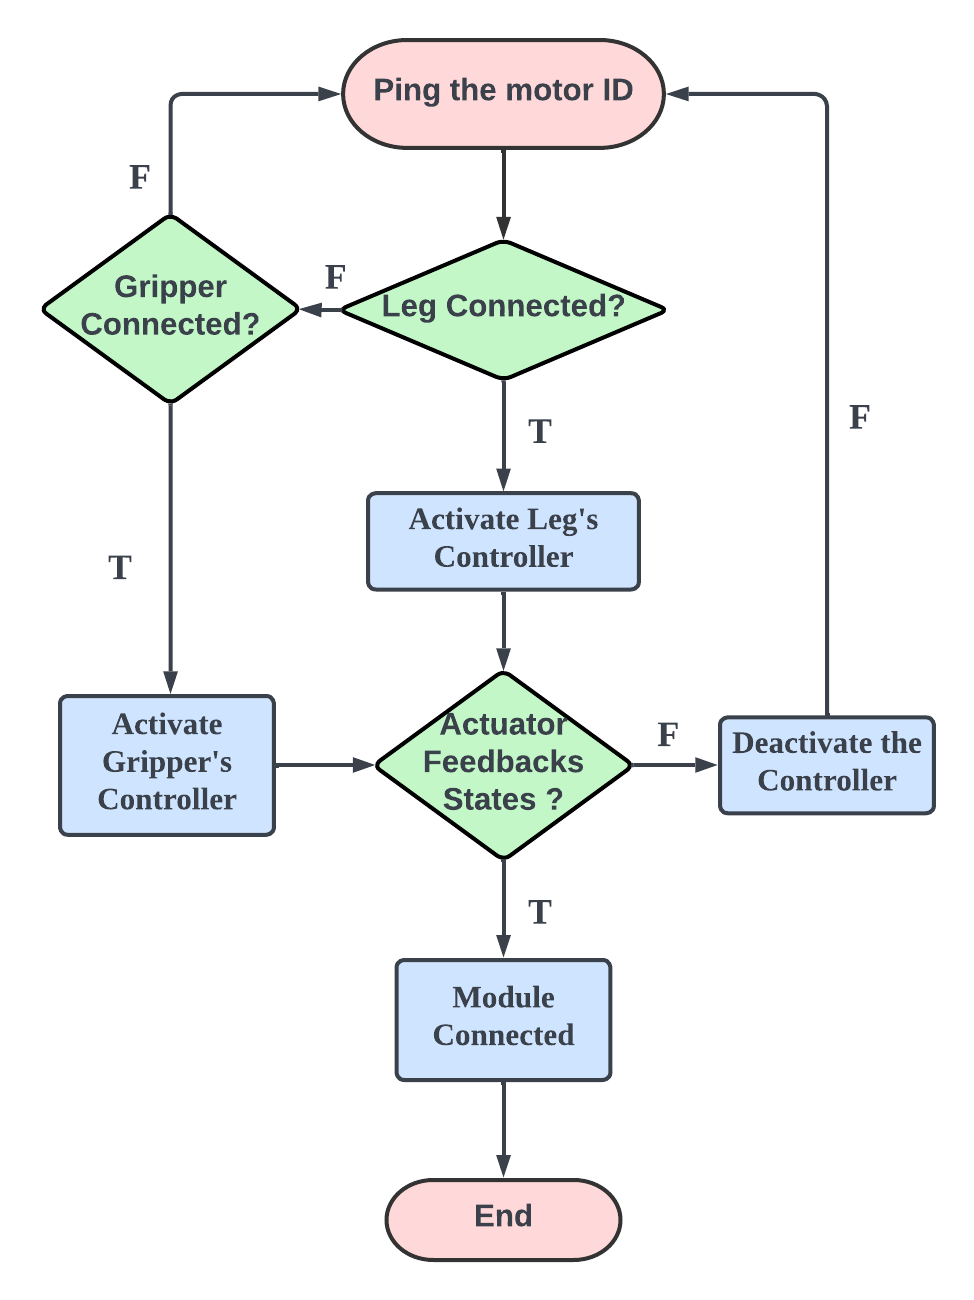
\includegraphics[width=90mm]{./fig/flowchart/flowchartcolor.png}
  \vspace{2mm}
  \caption{Self-recognition algorithm for each connection.}\label{flowchart}
\end{figure}

\begin{algorithm}[h]
\caption{Self-Recognition for module connection at right-rear port.}
\label{alg:module_recognition}
\begin{algorithmic}[1]
\Function{RR\_initializer\_callback}{}
    
    \If{\texttt{no RR\_module\_detected}}
        \If{\texttt{Found leg module at RR port}}
            \State \texttt{Activate leg's controller at RR port}
            % \State \texttt{RR\_detected = True}
            % \State \texttt{RR\_leg\_connected = True}
        \ElsIf{\texttt{Found gripper module at RR port}}
            \State \texttt{Activate gripper's controller at RR port}
            % \State \texttt{self.RR\_detected = True}
            % \State \texttt{self.RR\_gripper\_connected = True}
        % \Else
        %     \State \texttt{`No RR state detected!'}
        \EndIf
        
    \ElsIf{\texttt{RR\_module\_detected}}
        \If{\texttt{RR\_leg\_connected}}
            \If{\texttt{RR\_state error}}
                \State \texttt{Deactivate leg's controller at RR}
                % \State \texttt{RR\_leg\_connected = False}
                % \State \texttt{RR\_detected = False}
            % \Else
            %     \State \texttt{`RR CONNECTED!'}
            %     \State \texttt{RR\_detected = True}
            \EndIf
            
        \ElsIf{\texttt{RR\_gripper\_connected}}
            \If{\texttt{RR\_state error}}
                \State \texttt{Deactivate gripper's controller at RR}
                % \State \texttt{RR\_gripper\_connected = False}
                % \State \texttt{RR\_detected = False}
            % \Else
            %     \State \texttt{self.get\_logger().info(f"RR CONNECTED!")}
            %     \State \texttt{self.RR\_detected = True}
            \EndIf
        \EndIf
    \EndIf
\EndFunction
\end{algorithmic}
\end{algorithm}

\subsection{Node Structure and Components}
The controller of the Moonbot are separated for each connector, including limbs—RF (Right Front), LF (Left Front), LR (Left Rear), and RR (Right Rear) as shown in \fig{mb_control}. From this structure, to control the motion, four launching services are needed to be implemented for each controller. With the framework of ROS2 control, we can handled the command and state of each joint independently. Consequently, the module detection node handle the joint states of four specific ports, separately. \\
% \vspace{5mm}

\begin{figure}[h]
  \centering
  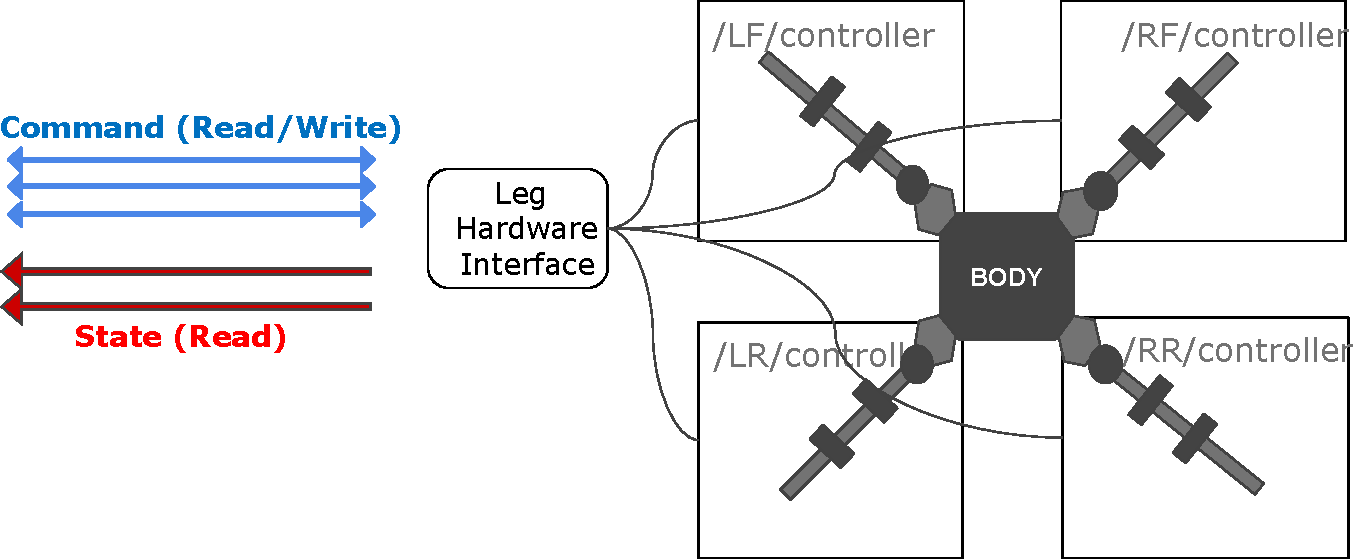
\includegraphics[width=140mm]{./fig/chap3/control_system/mb_control2.pdf}
  \vspace{2mm}
  \caption{Separated controller for each module.}\label{mb_control}
\end{figure}

% \subsection{Flowchart \& Algorithms}


\subsection{Initialization Process}
The initialization process is involved with activation of the controller into the life cycle of control, as we have discussed in the section of controller manager.

Upon initiation, the nodes for module detection check the availability of the corresponding hardware by attempting to communicate with the actuators (pinging). The communication is established through Dynamixel motors with the specific ID number. After the success of this communication, the module detection node sends the request to the service server that handle the launch service of actuator activation.  

% In addition, the state of the motors is the key parameter for monitoring the existence of module connection.

\subsection{Periodic Connection Status Monitoring}
% Following the initialization, the node continuously monitors the joint states of each module at regular intervals. The joint states provide information about the current position of the limbs' joints. This periodic monitoring is facilitated by timer callbacks dedicated to each limb. 

% In addition, the motors status monitoring also functions as a error detector. If the joint position of a limb deviates beyond a predefined threshold, which occurs when the motors is not connected and the states are unreadable, it indicates a potential issue such as disconnection or misalignment. In such cases, the node dynamically updates the connection status for that module.

% Unfortunately, the current version of \textit{hardware\_interface} in ROS2 control has not been implemented with the restart function feature for lost hardware yet. Therefore, the launch services contain the function to automatically shutdown the process of controller manager which means disconnection the hardware from the software control. If the hardware is reconnected to the connector and is detected, the program operates the same process as the initialization and relaunch the activity of ROS2 control again.

Following the initialization, the node continuously monitors the joint states of each module at regular intervals, providing real-time information on the current position of the limbs' joints. Timer callbacks dedicated to each limb facilitate this periodic monitoring.

Additionally, the node functions as an error detector by monitoring the status of the motors. If a joint position deviates beyond a predefined threshold, indicating potential issues like disconnection or misalignment, the node dynamically updates the connection status for that module.

However, it's worth noting that the current version of the \textit{hardware\_interface} in ROS2 control does not include a restart function for lost hardware. Therefore, the launch services incorporate a feature to automatically shut down the controller manager process in response to hardware disconnection. Upon reconnecting the hardware, the program reinitializes the ROS2 control activity, relaunching the controller manager process.

\subsection{Adaptability to Grippers}
The Dynamixel motors offer a unique ID identification feature, accessible through the Dynamixel Wizard GUI tool \cite{dynamixel_wizard2}, which facilitates initial setup. In Moonbot's control system, the module detection node is designed to identify specialized components, such as grippers, by searching for specific motor IDs. For instance, a motor ID of 1 corresponds to the leg module, while an ID of 2 signifies the gripper module. By extending self-recognition capabilities to include end-effectors, we enhance the versatility of our robotic system.\\

\begin{figure}[h]
  \centering
  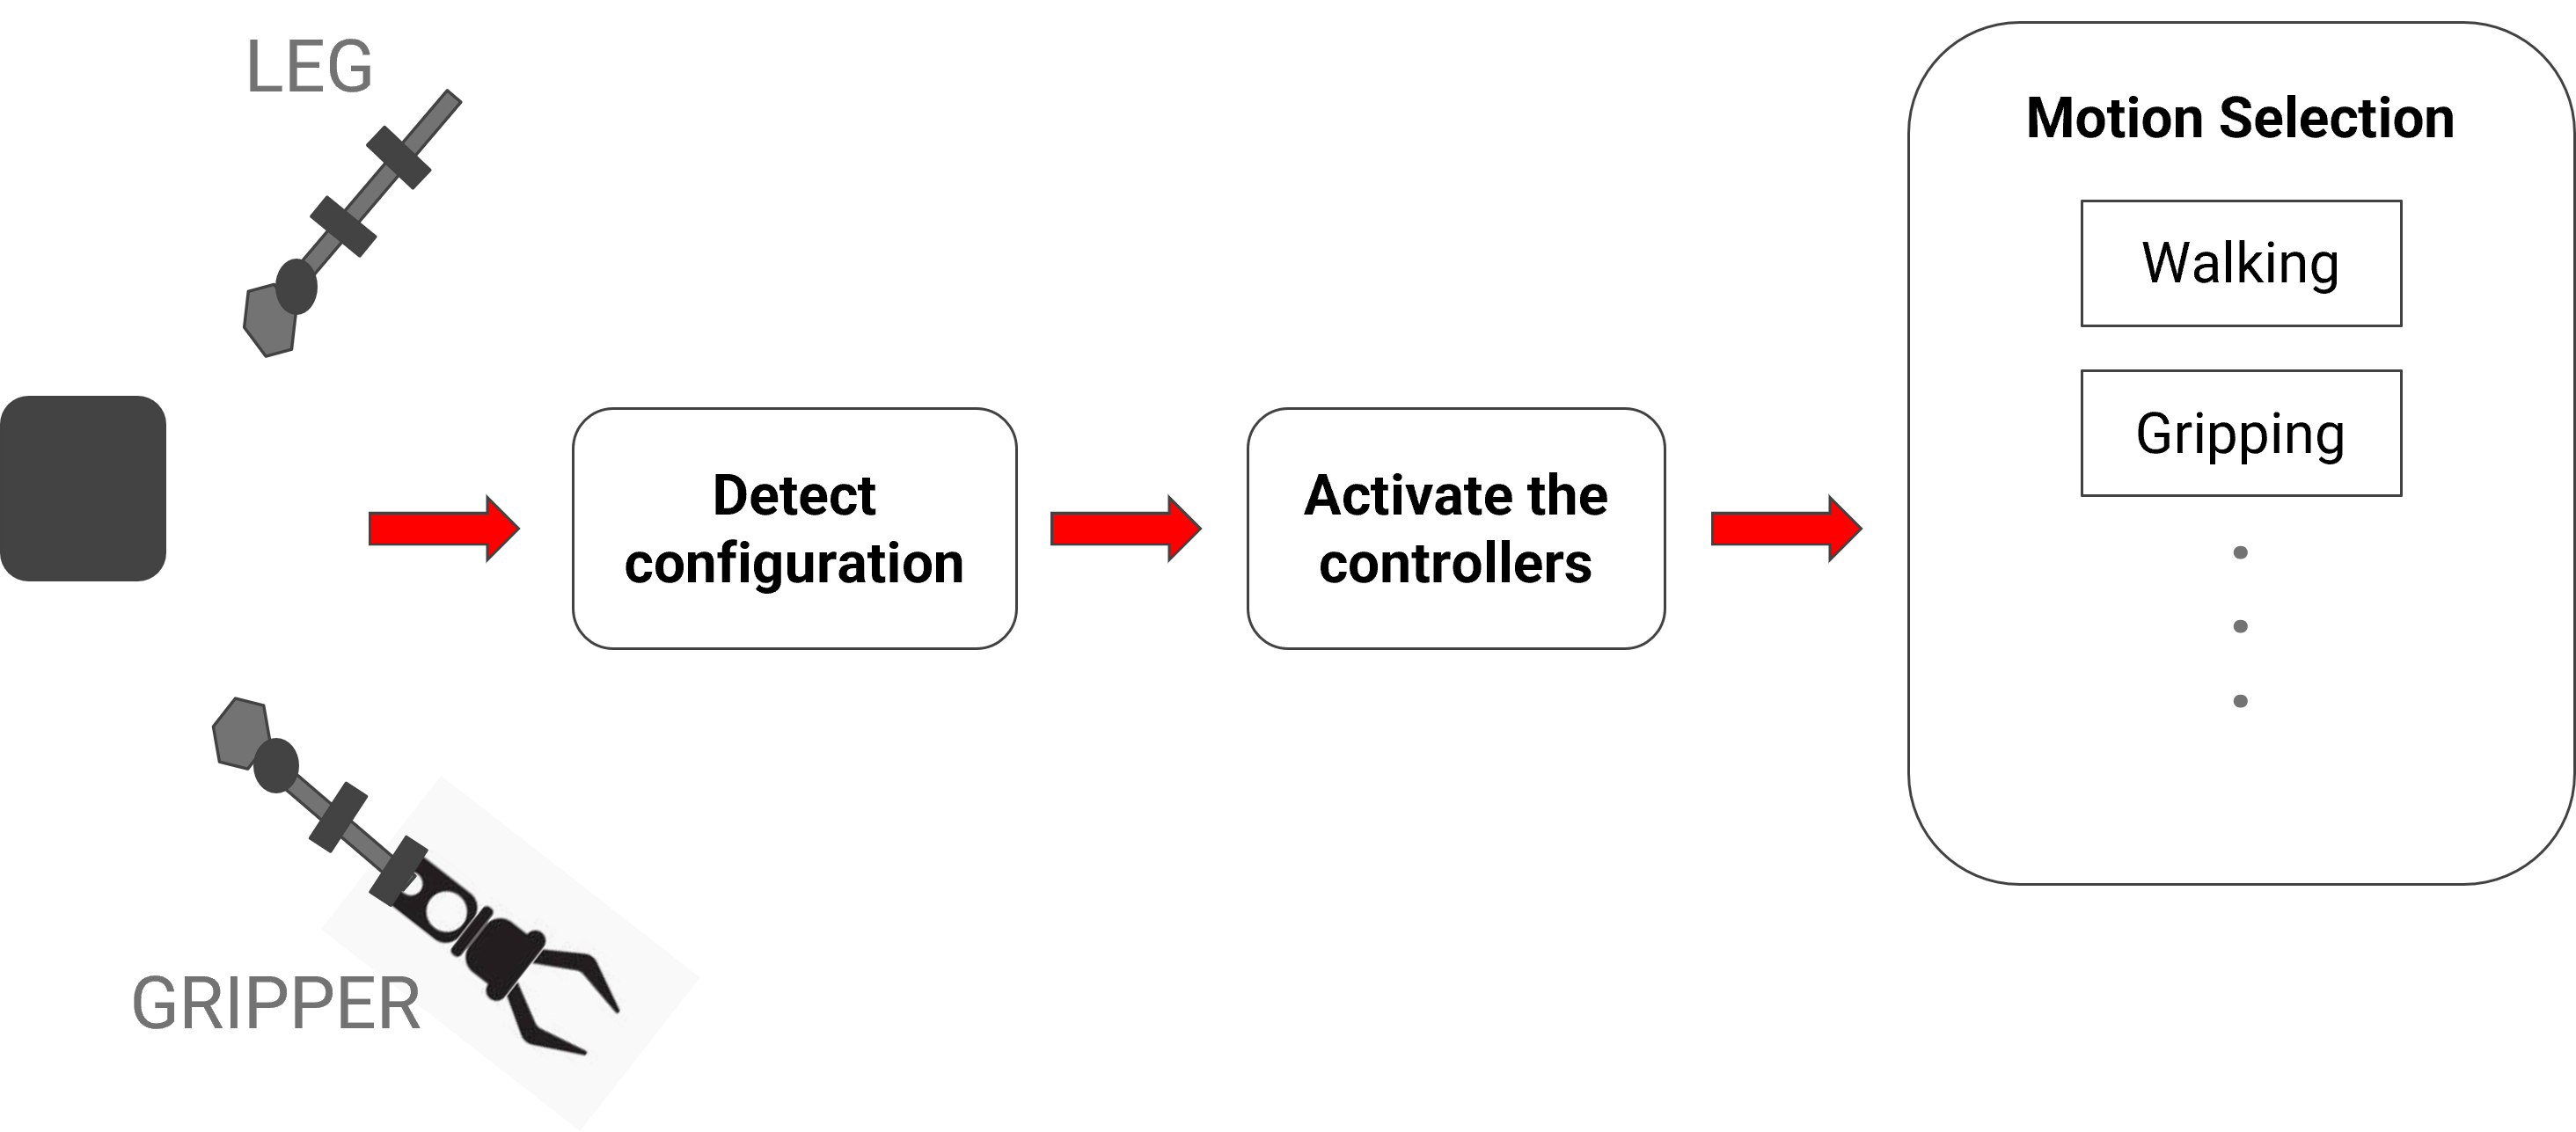
\includegraphics[width=130mm]{./fig/chap3/control_system/leggrip.png}
  \vspace{2mm}
  \caption{Motion selection depending on module type.}\label{gripleg}
\end{figure}

\subsection{Motion Selection}
After the implementation of connection recognition of the module is success, the self-recognition algorithm can report the connection status of each connector in real-time, periodically. From this information, we can perform an experiment for motion selection depending on Moonbot configuration's which are mentioned in the problem statements.

To present the adaptability of the modular legged robot, Moonbot's locomotion styles including crawling motion and walking motion. The motion style is selected by the number of leg module connection.

\label{enumerate}
\begin{enumerate}
\item \textit{Crawling Motion:}
Moonbot moves by crawling motion when operating with a single-leg configuration towards the direction of connected module. Extending its capabilities, two-legged and three-legged configuration, Moonbot move with the same style as single configuration, but higher power by more legs applied.\\


\begin{figure}[h]
  \centering
  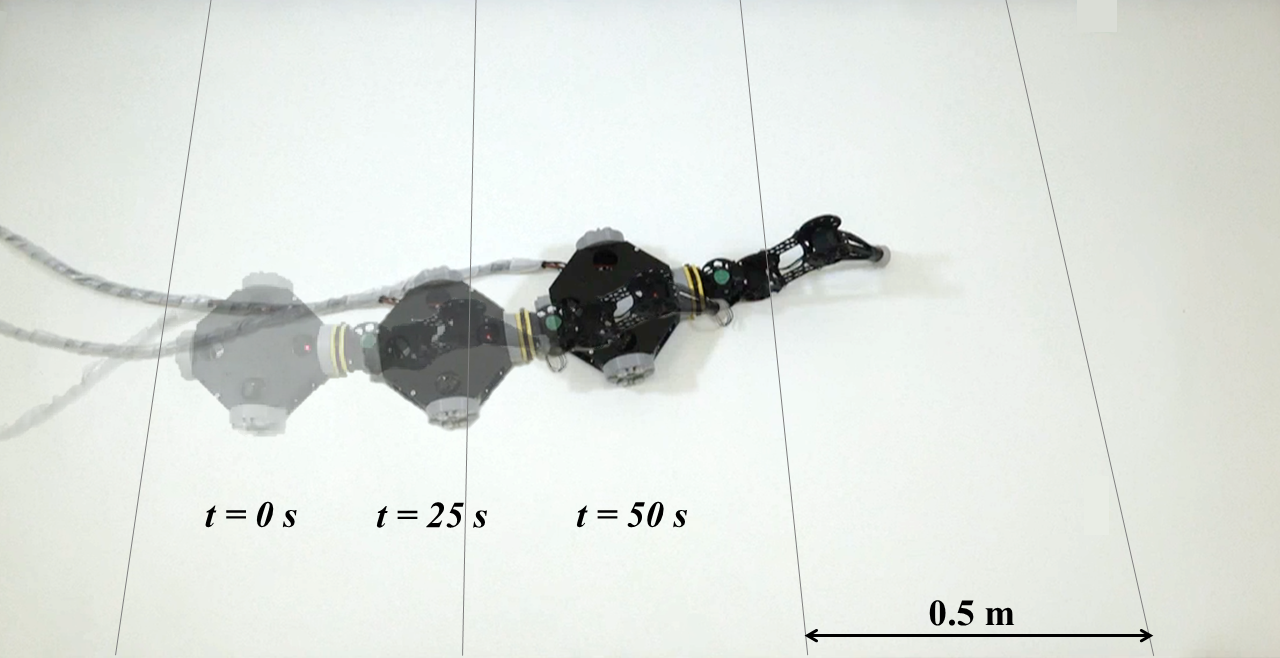
\includegraphics[width=110mm]{./fig/chap3/snapshot/single_snapshot4.png}
  \vspace{2mm}
  \caption{Snapshots of crawling motion for single-leg configuration.}\label{singlesnap}
\end{figure}


% \begin{figure}[h]
%   \centering
%   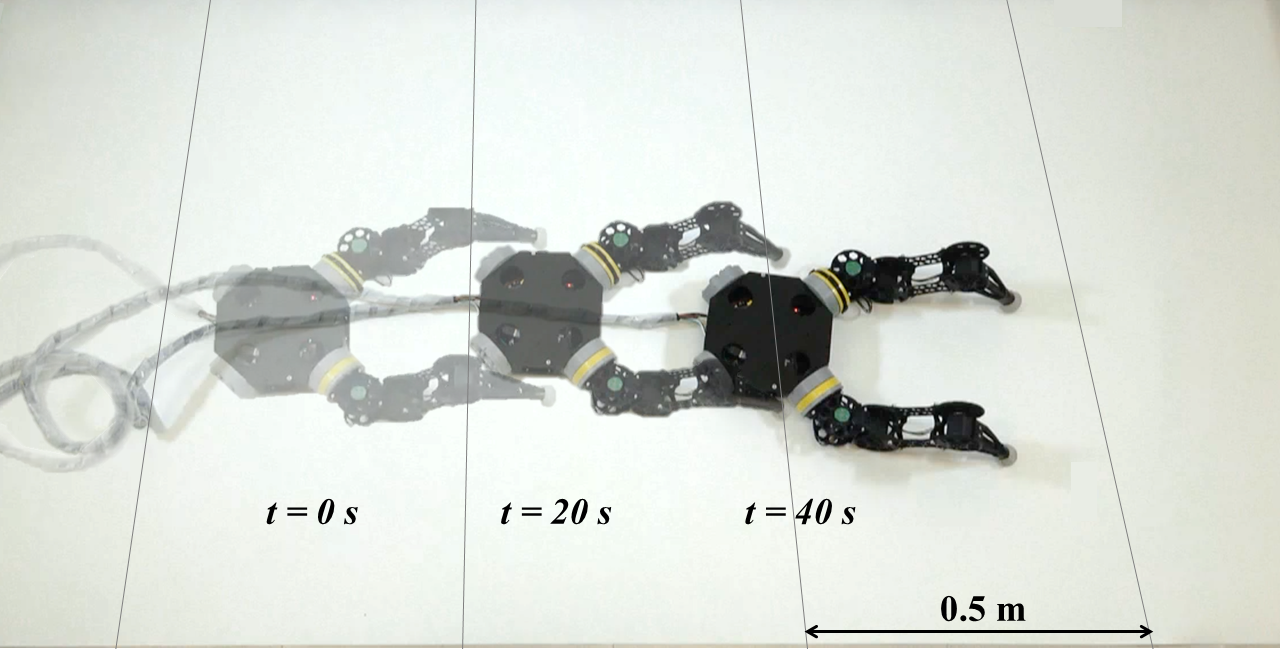
\includegraphics[width=110mm]{./fig/chap3/snapshot/double_snapshot3.png}
%   \vspace{2mm}
%   \caption{Snapshots of crawling motion for double-leg configuration.}\label{doublesnap}
% \end{figure}

% \begin{figure}[h]
%   \centering
%   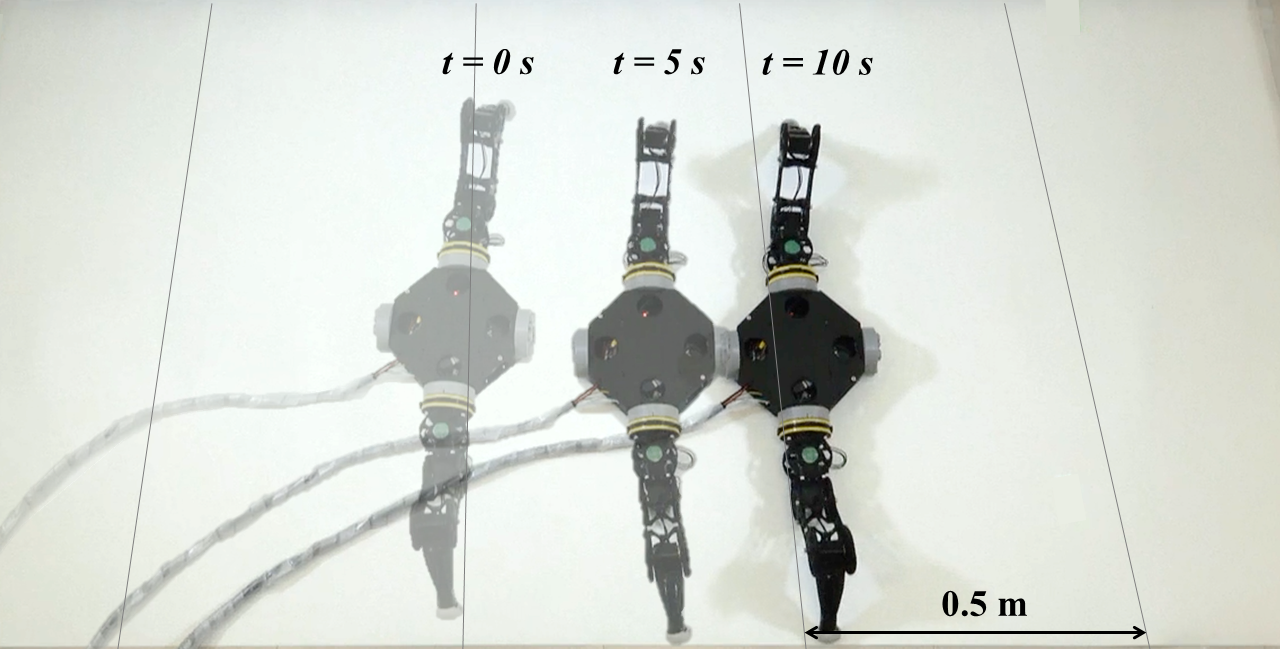
\includegraphics[width=110mm]{./fig/chap3/snapshot/double_snapshot4.png}
%   \vspace{2mm}
%   \caption{Snapshots of crawling motion for double-leg at opposite ports configuration.}\label{doublesnap2}
% \end{figure}

\begin{figure}[h]
 \begin{subfigure}{1.0\textwidth}
 \begin{center}
  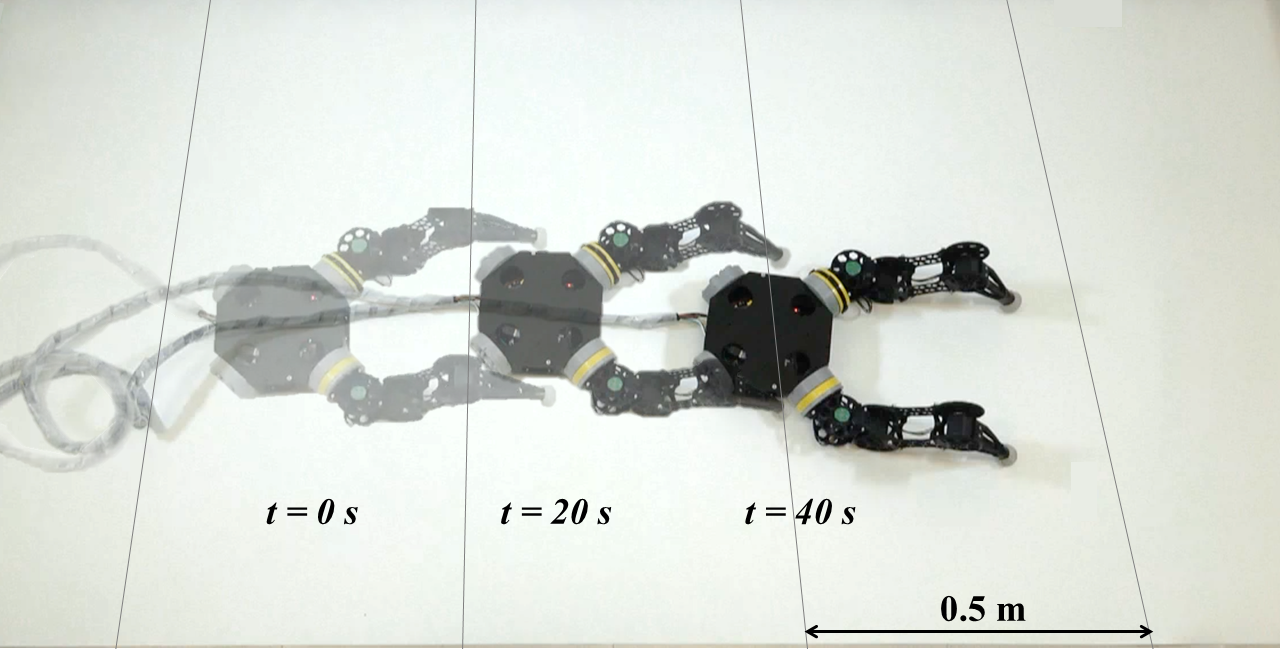
\includegraphics[width=110mm]{./fig/chap3/snapshot/double_snapshot3.png}
% \vspace{2mm}
  \caption{Crawling motion for double-leg configuration.}\label{doublesnap1}
 \end{center}
 \end{subfigure}
 
 \begin{subfigure}{1.0\textwidth}
 \begin{center}
  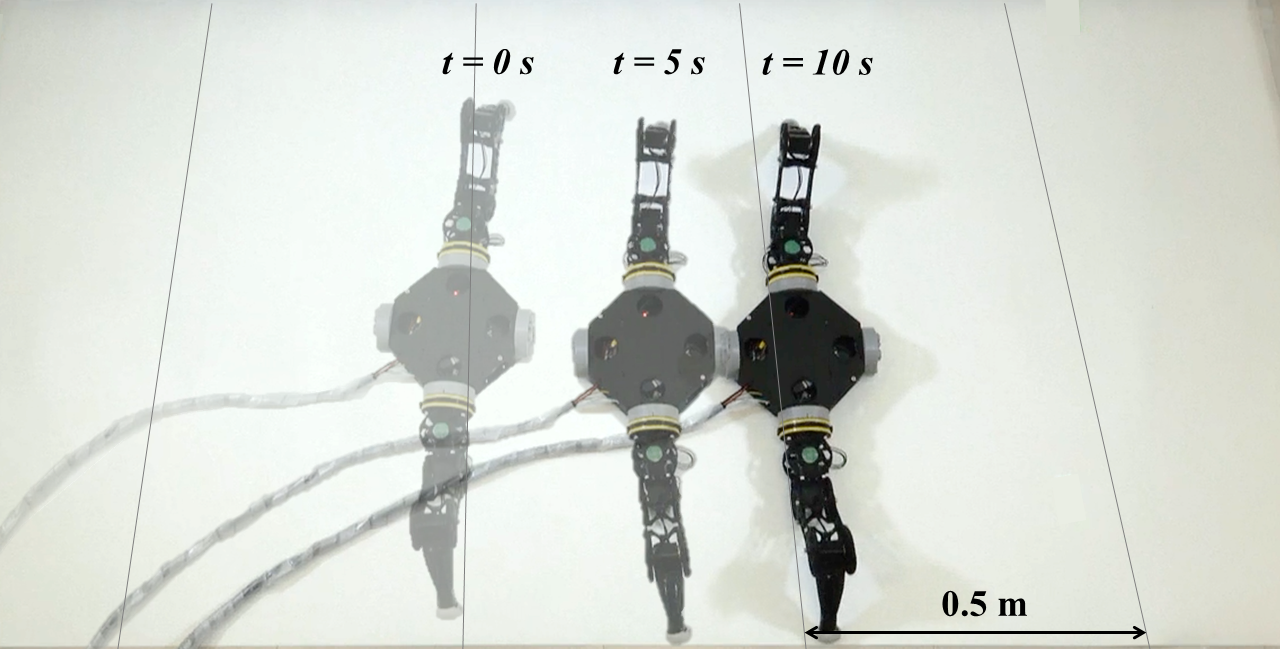
\includegraphics[width=110mm]{./fig/chap3/snapshot/double_snapshot4.png}
% \vspace{2mm}
  \caption{Crawling motion for double-leg at opposite ports configuration.}\label{doublesnap2}
\end{center}
\end{subfigure}
\vspace{-2mm}
\caption{Snapshots of crawling motion for double-leg configuration.}
\label{doublesnap}
\end{figure}




% \begin{figure}[h]
%  \centering
%  \begin{subfigure}{0.2\textwidth}
%  \begin{center}
%   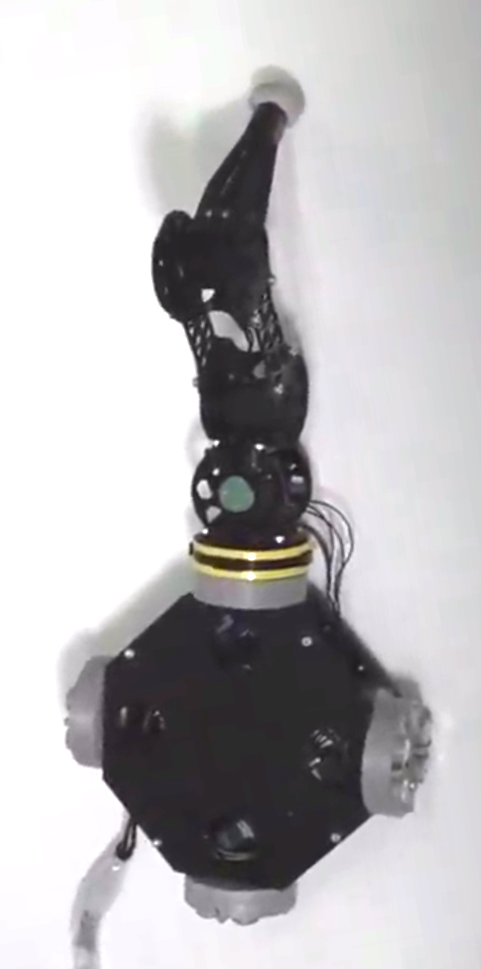
\includegraphics[width=25mm]{./fig/locomotion/11.png}
% \caption{Neutral pose}\label{snapshot1.1}
%  \end{center}
%  \end{subfigure}
%  \begin{subfigure}{0.2\textwidth}
%  \begin{center}
%   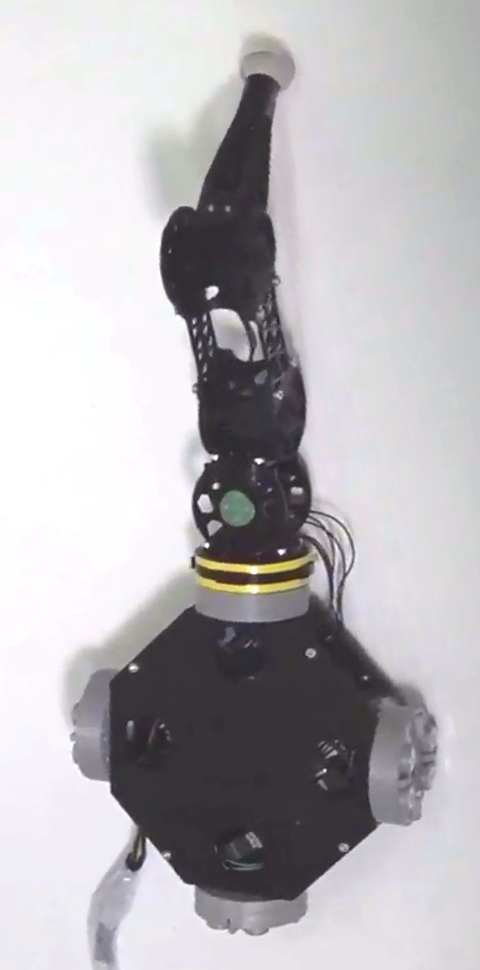
\includegraphics[width=25mm]{./fig/locomotion/12.png}
% \caption{Stretch the leg}\label{snapshot1.2}
% \end{center}
% \end{subfigure}
%  \begin{subfigure}{0.2\textwidth}
%  \begin{center}
%   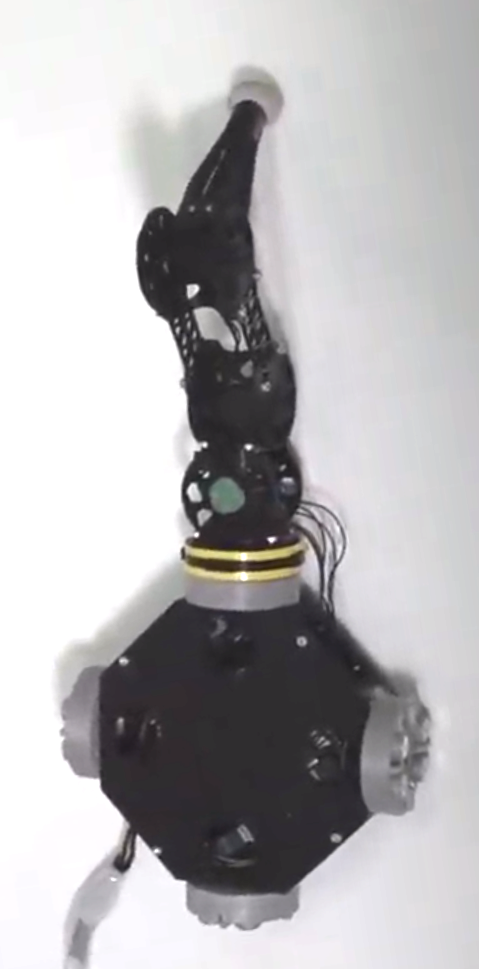
\includegraphics[width=25mm]{./fig/locomotion/13.png}
% \caption{Pulling forward}\label{snapshot1.3}
%  \end{center}
%  \end{subfigure}
% \vspace{-1mm}
% \caption{Crawling motion for single-leg configuration}
% \label{snap1}
% \end{figure}

% \begin{figure}[h]
%  \centering
%  \begin{subfigure}{0.2\textwidth}
%  \begin{center}
%   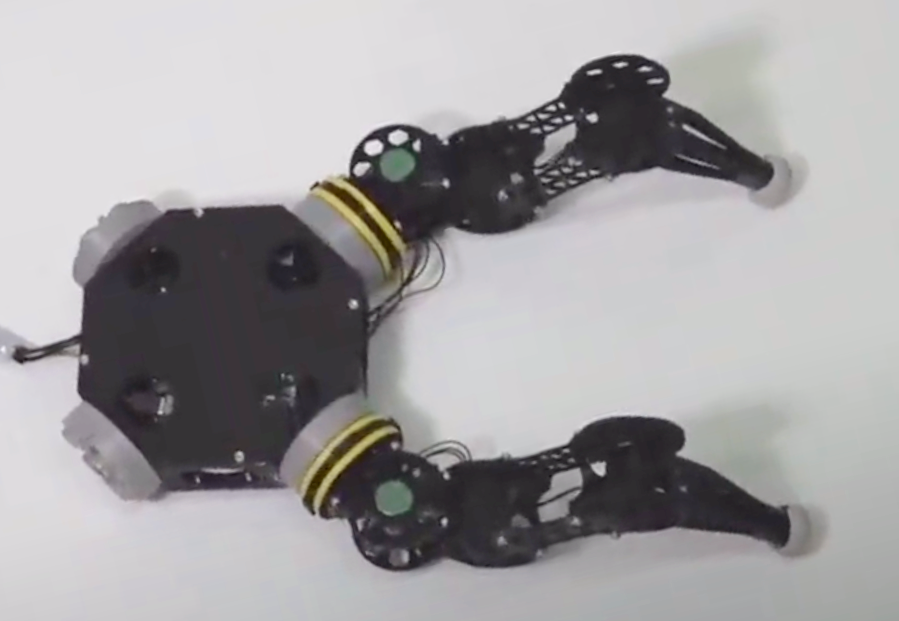
\includegraphics[width=40mm, angle=90]{./fig/locomotion/21.png}
% \caption{Neutral pose}\label{snapshot2.1}
%  \end{center}
%  \end{subfigure}
%  \begin{subfigure}{0.2\textwidth}
%  \begin{center}
%   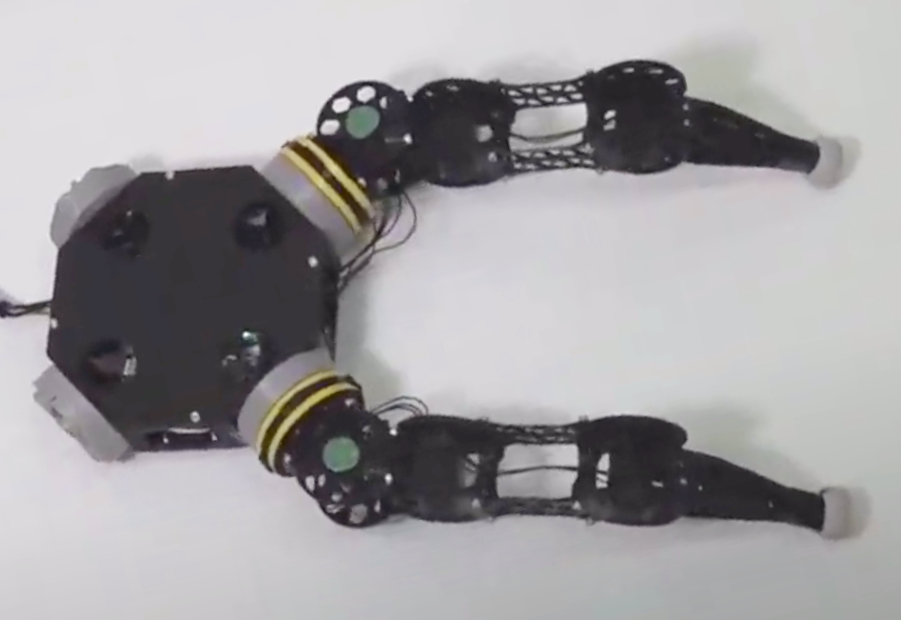
\includegraphics[width=40mm, angle=90]{./fig/locomotion/22.png}
% \caption{Stretch the leg}\label{snapshot2.2}
% \end{center}
% \end{subfigure}
%  \begin{subfigure}{0.2\textwidth}
%  \begin{center}
%   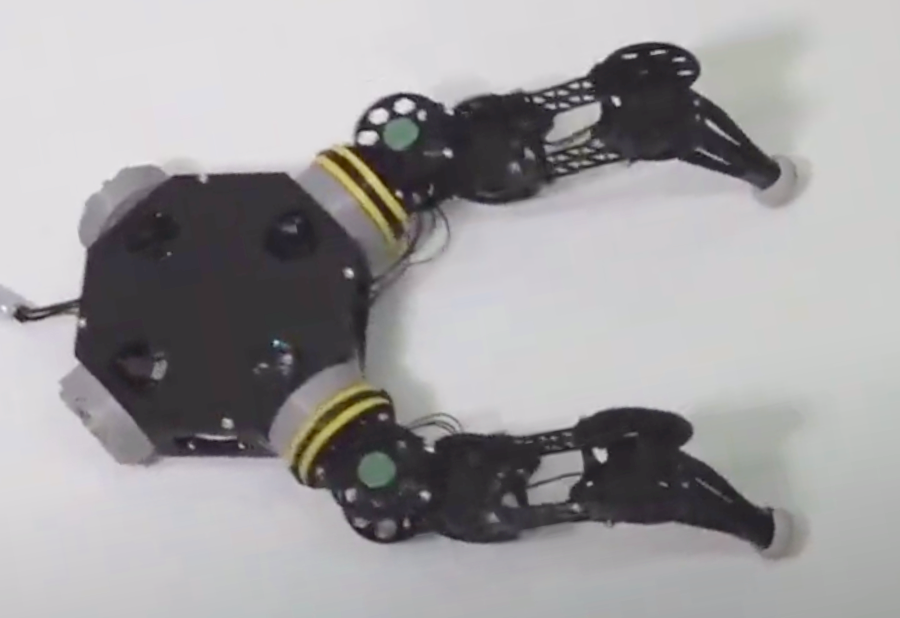
\includegraphics[width=40mm, angle=90]{./fig/locomotion/23.png}
% \caption{Pulling forward}\label{snapshot2.3}
%  \end{center}
%  \end{subfigure}
% % \vspace{-1mm}
% \caption{Crawling motion for double-leg configuration}
% \label{snap2}
% \end{figure}



\item \textit {Walking motion:}
In full configuration, employing all four legs, is designed for versatile locomotion. Moonbot can perform both a crawl gait for static stability and a trot gait for a more dynamic walking motion. \\
% \begin{itemize}
%     \item \textbf{Crawl gait}: Provides static stability by moving one or more legs at a time while maintaining contact with the ground. This gait is well-suited for navigating rough or uneven terrain where stability is crucial.

%     \item \textbf{Trot gait}: Offers a more dynamic walking motion by coordinating the movement of diagonally opposite legs. This gait allows for faster locomotion and is suitable for traversing relatively flat or open terrain.
% \end{itemize}

\begin{figure}[h]
  \centering
  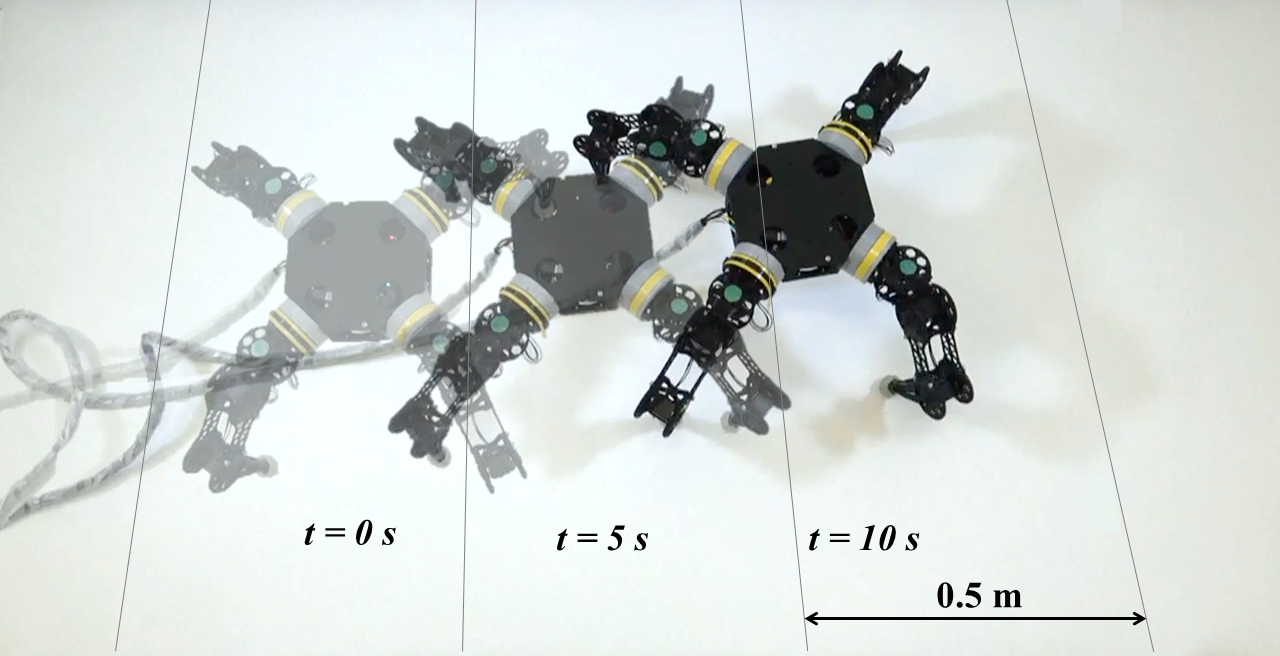
\includegraphics[width=110mm]{./fig/chap3/snapshot/full_snapshot4.png}
  \vspace{2mm}
  \caption{Snapshots of walking motion in self-recognition test.}\label{fullsnap}
\end{figure}

%%%
% \begin{figure}[h]
%   \centering
%   \begin{minipage}[ht]{0.2\textwidth}
%     \centering
%     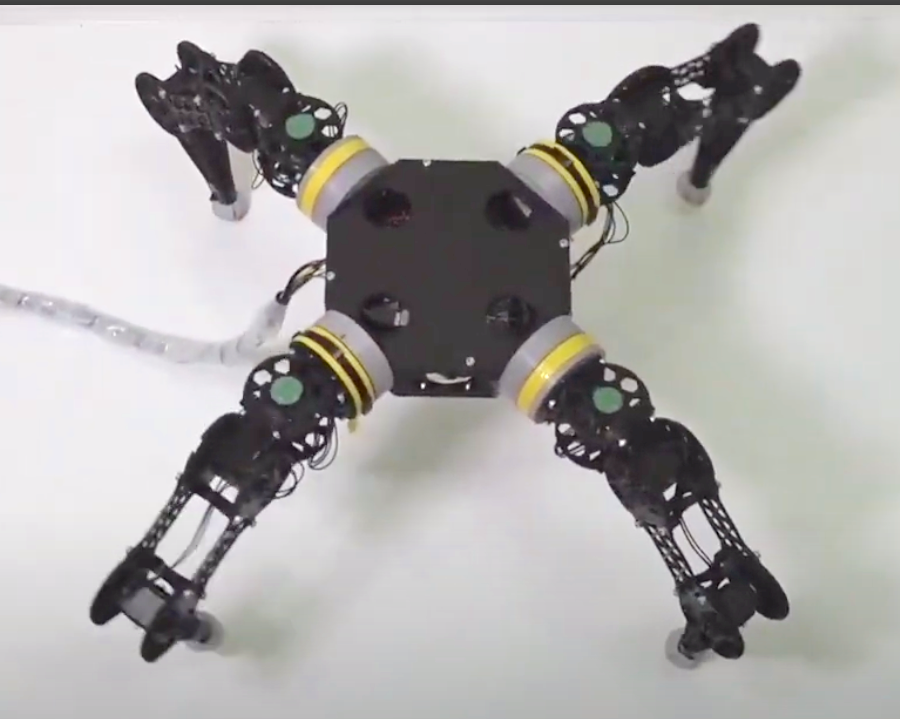
\includegraphics[clip, width=30mm]{./fig/locomotion/40.png}
%   \end{minipage}
%   \begin{minipage}[ht]{0.2\textwidth}
%     \centering
%     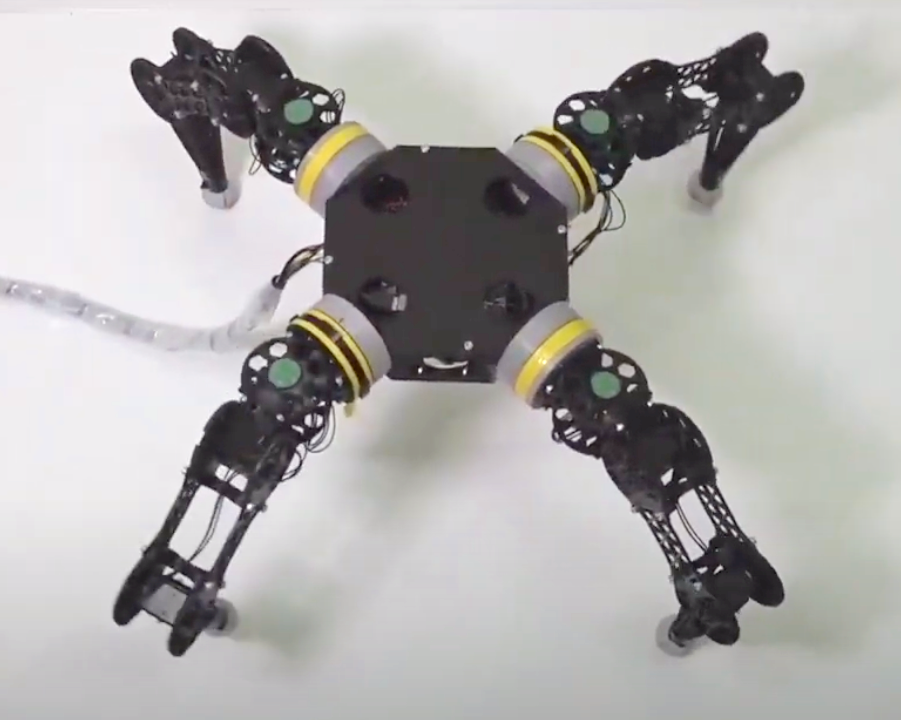
\includegraphics[clip, width=30mm]{./fig/locomotion/41.png}
%   \end{minipage}
%   \begin{minipage}[ht]{0.2\textwidth}
%     \centering
%     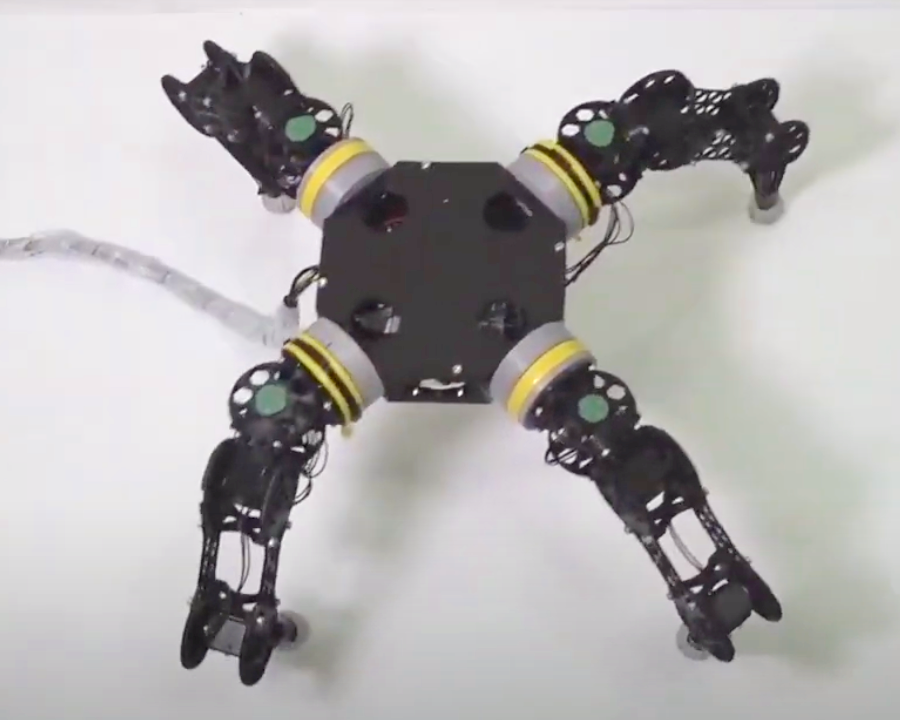
\includegraphics[clip, width=30mm]{./fig/locomotion/42.png}
%   \end{minipage}
%   \begin{minipage}[ht]{0.2\textwidth}
%     \centering
%     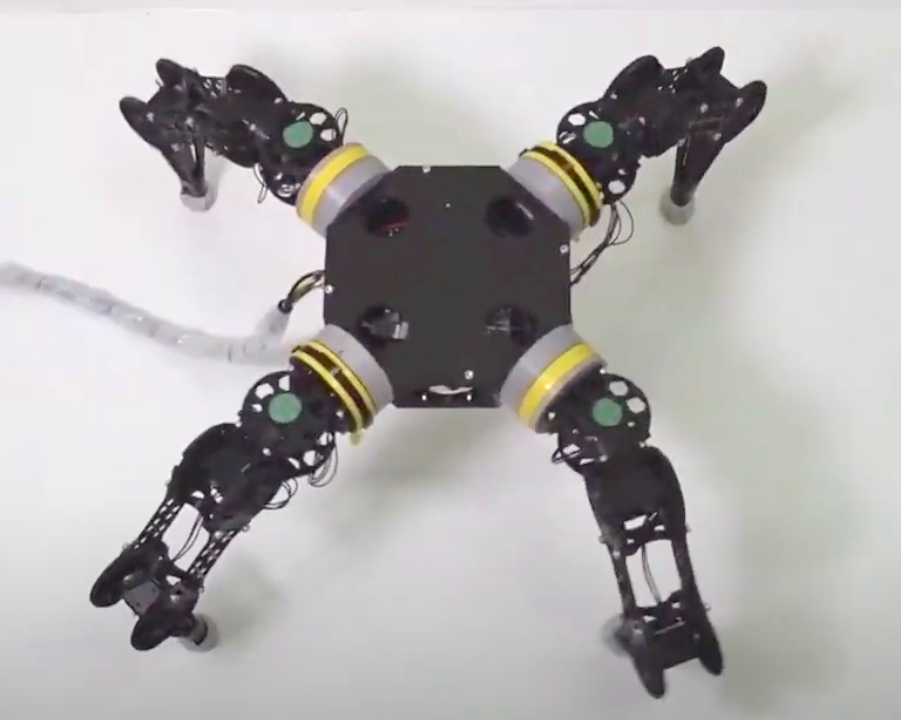
\includegraphics[clip, width=30mm]{./fig/locomotion/43.png}
%   \end{minipage}\\
%   \begin{minipage}[ht]{0.2\textwidth}
%     \centering
%     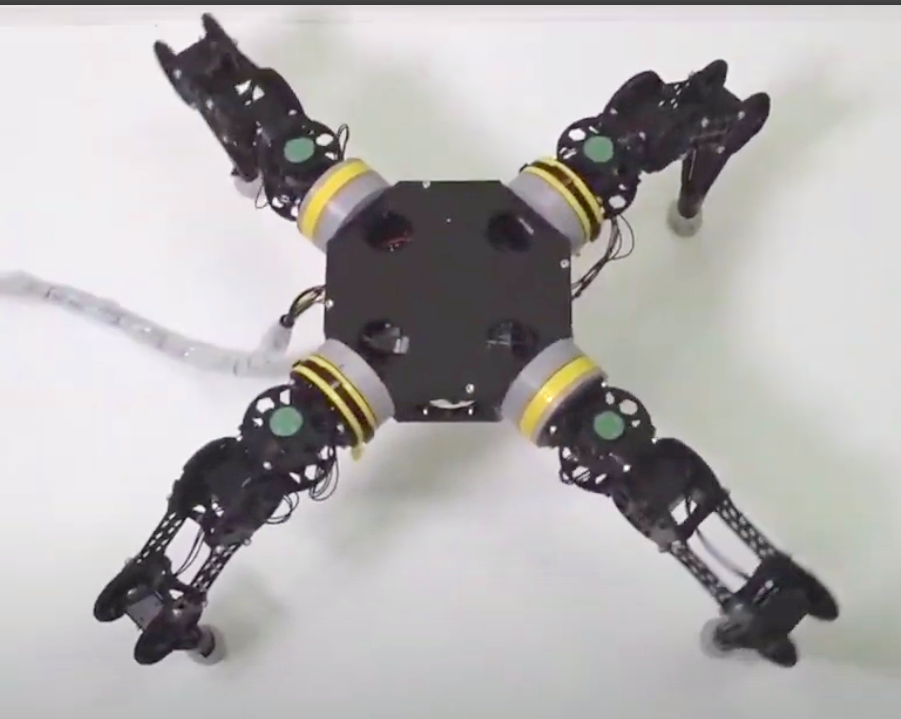
\includegraphics[clip, width=30mm]{./fig/locomotion/44.png}
%   \end{minipage}
%   \begin{minipage}[ht]{0.2\textwidth}
%     \centering
%     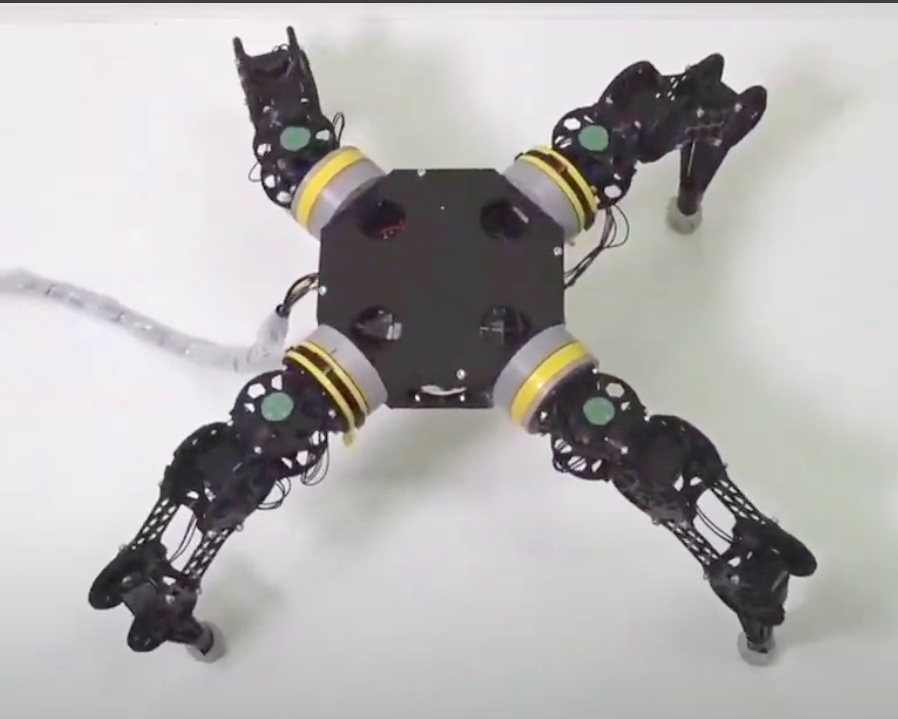
\includegraphics[clip, width=30mm]{./fig/locomotion/45.png}
%   \end{minipage}
%   \begin{minipage}[ht]{0.2\textwidth}
%     \centering
%     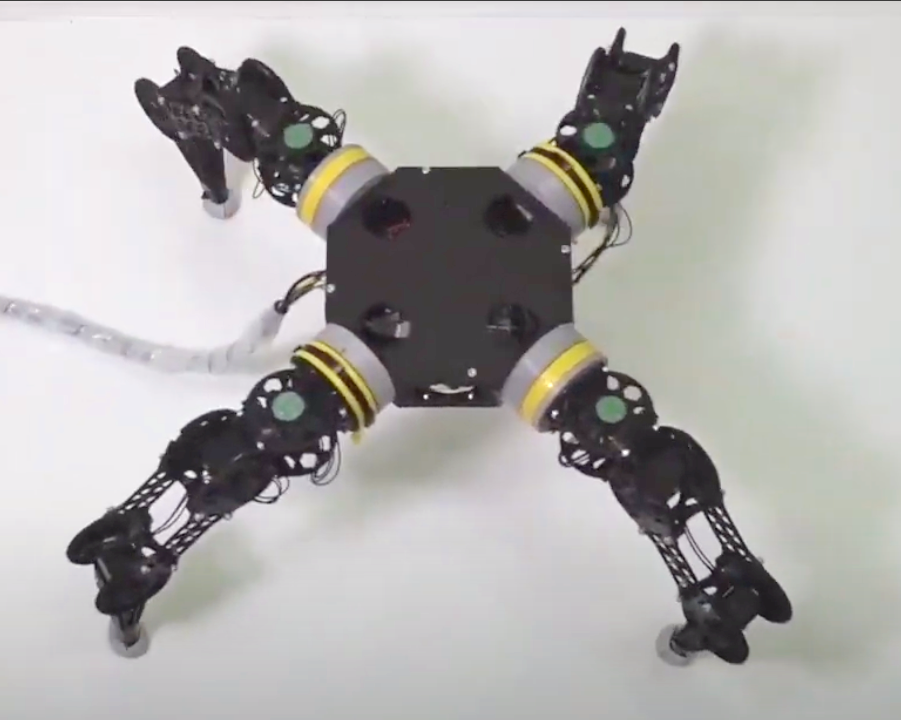
\includegraphics[clip, width=30mm]{./fig/locomotion/46.png}
%   \end{minipage}
%   \begin{minipage}[ht]{0.2\textwidth}
%     \centering
%     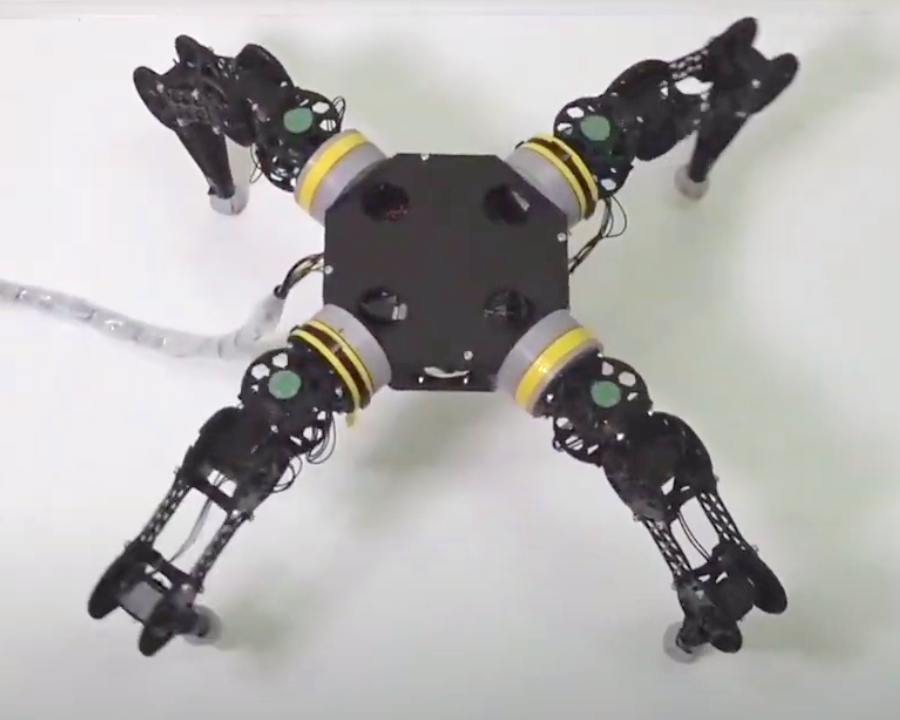
\includegraphics[clip, width=30mm]{./fig/locomotion/47.png}
%   \end{minipage}
% \caption{Walking motion}
% \label{minipage}
% \end{figure}
\end{enumerate}

In addition to the number of module, the type of module also a parameter for motion selection. Moonbot's module contain both leg type and gripper type. By finding the ID dynamixel motor labeled as a gripper type, the robot can recognize the connection of gripper and perform a motion task such as waving and gripping the gripper.\\

\begin{figure}[h]
  \centering
  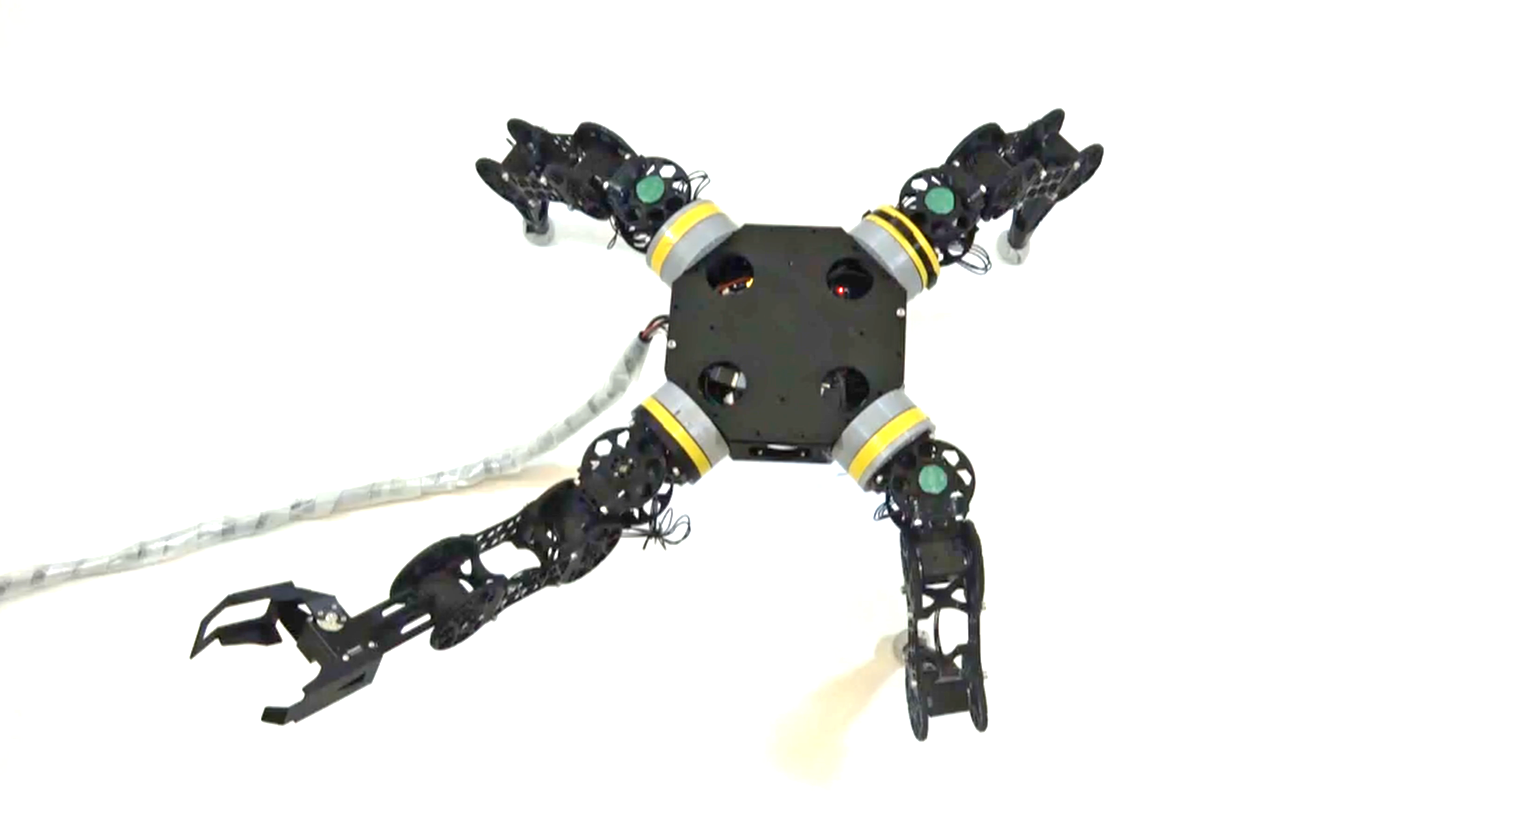
\includegraphics[width=110mm]{./fig/moonbot/grippermoonbot.png}
  \vspace{2mm}
  \caption{Gripper module connect with the Moonbot.}\label{Moonbot gripper}
\end{figure}

\begin{figure}[t]
  \centering
  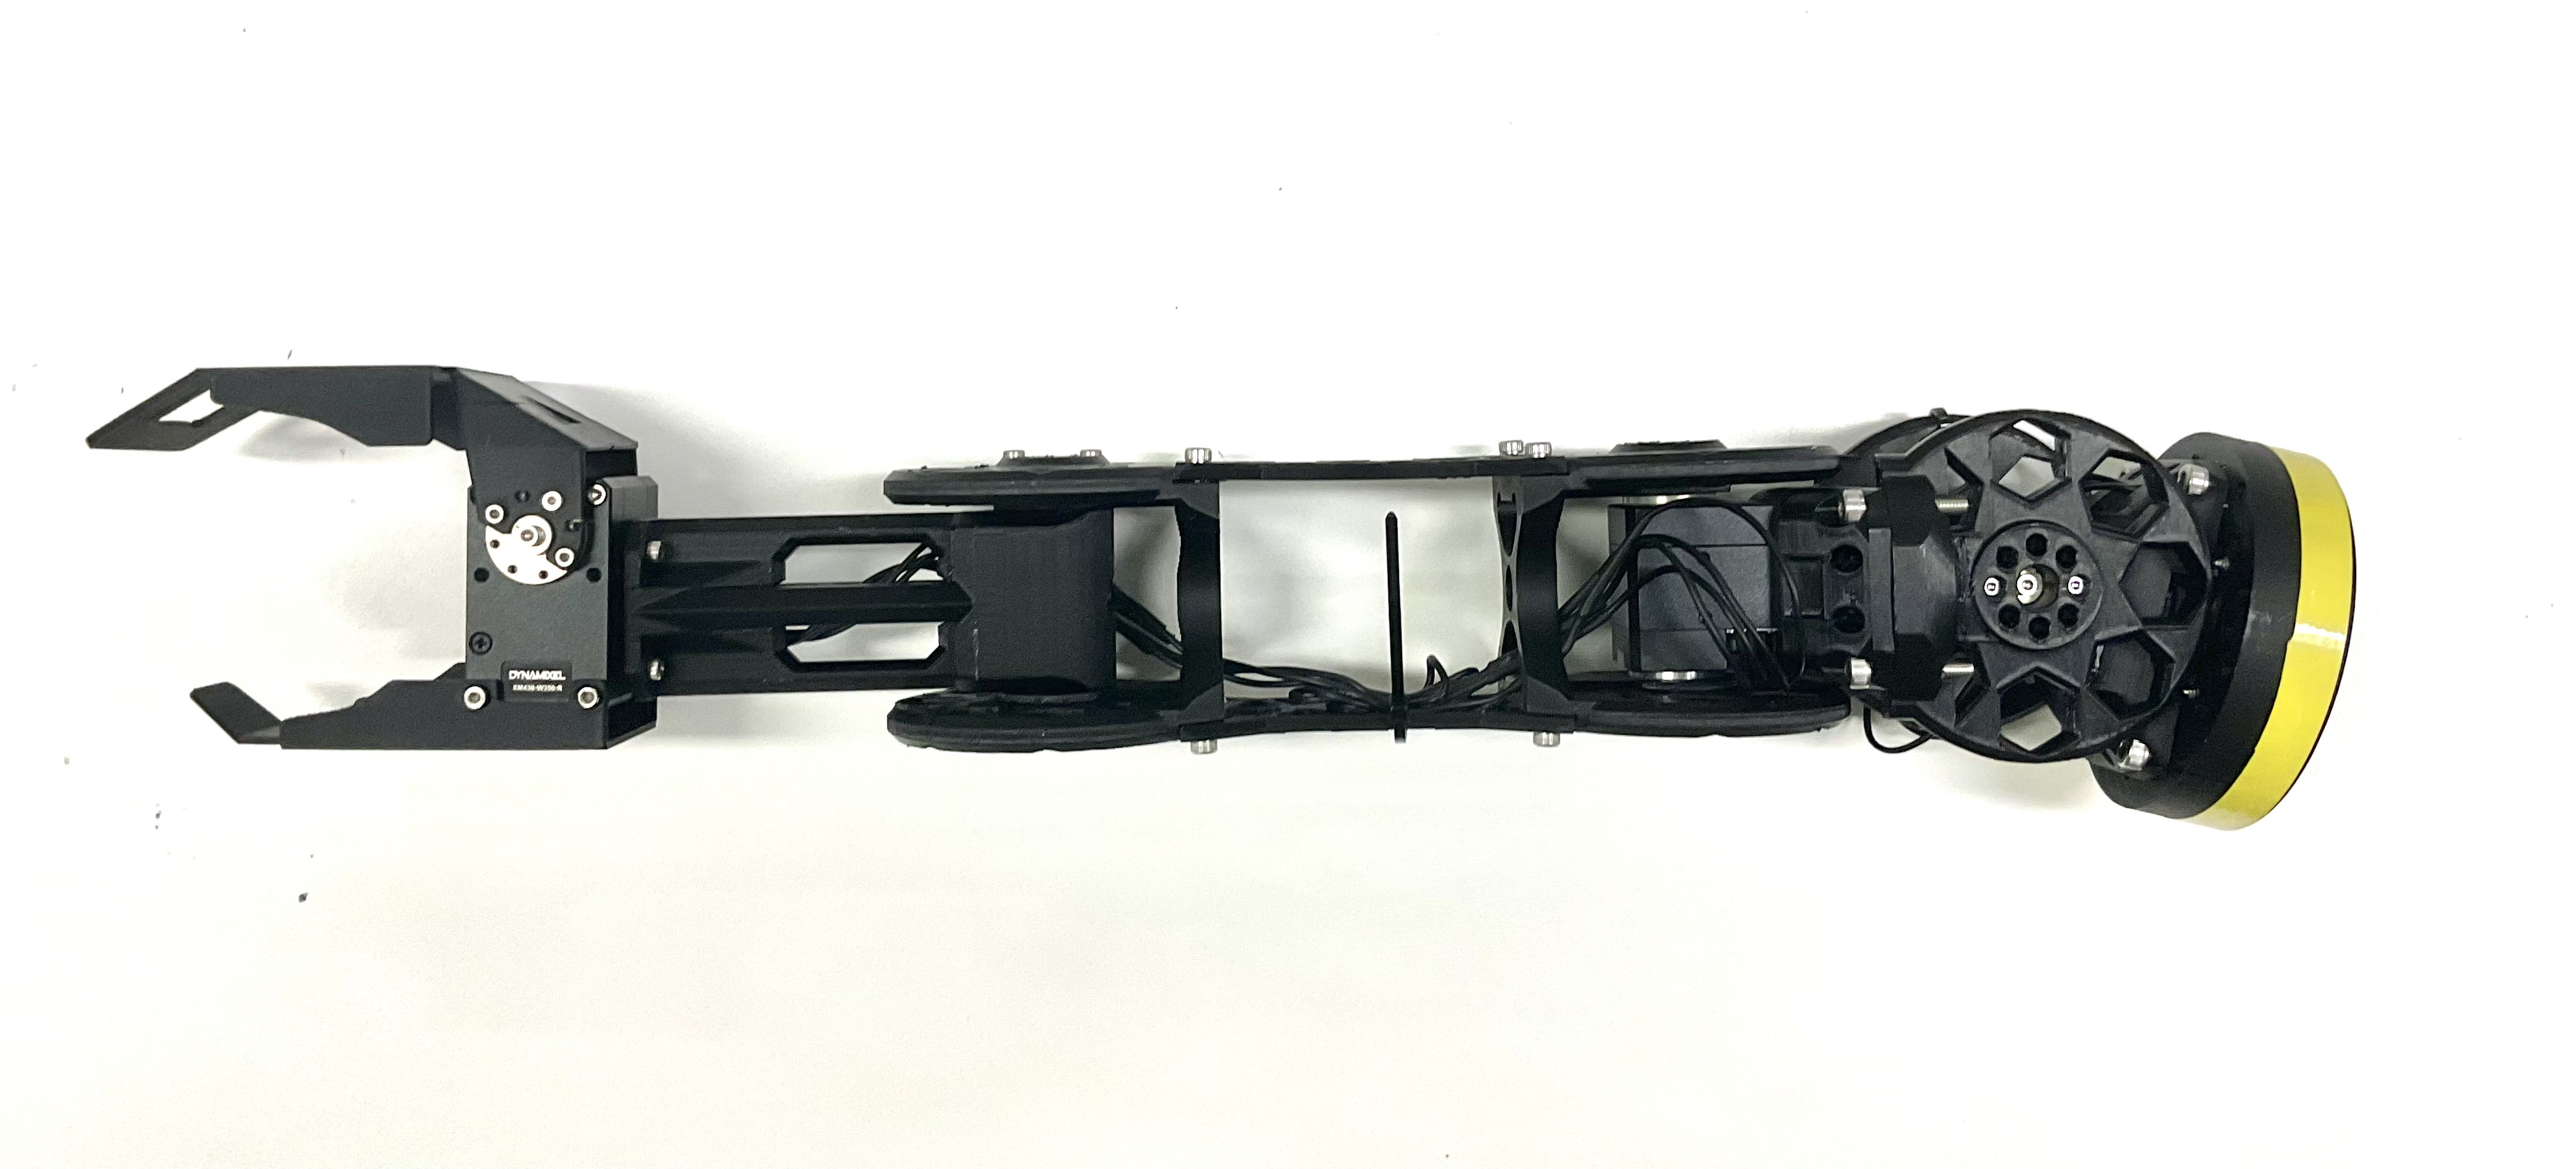
\includegraphics[width=90mm]{./fig/leg_configuration/gripper_module.jpg}
  \vspace{2mm}
  \caption{Motion selection depending on module type.}\label{gripmodule}
\end{figure}

%%% EOF %%%

\chapter{Motion Control}
%\label{cha:CCCC}
%%%%%%%%%%%%%%%%%%%%%%%%%%%%%%%%%%%%%%%%%%%%%%%%%%%%%%%%%
%%%
%%%  第4章
%%%  参考文献の表示
%%%
%%%%%%%%%%%%%%%%%%%%%%%%%%%%%%%%%%%%%%%%%%%%%%%%%%%%%%%%%
% \section{Locomotion \& Motion Selection}
This section drives into the locomotion strategy for Moonbot with full configuration operation. The motion control is orchestrated through the integration of ROS2 control framework. The joint trajectory controller is used to operate the multiple joints.

\section{Joint Trajectory Controller}
ROS2 control offers a versatile tool called \texttt{ros2\_controllers} \cite{ros2controllers}, designed as a controller interface accommodating various robot specifications. For example, the \texttt{position\_controller} can accept position inputs and generate corresponding outputs to a position interface. Similarly, the \texttt{velocity\_controller} receives input and produces velocity output. Additionally, specialized controllers like the \texttt{diff\_drive\_controller} provide advanced control interfaces tailored for mobile robots equipped with wheeled locomotion systems.

For precise control of Moonbot's dynamic locomotion, the \texttt{joint\_trajectory\_controller} from ROS2 is utilized. This controller executes joint-space trajectories on multiple joints, enabling smooth and dynamic locomotion by interpolating the waypoints to desired target at specific time. 

There are three strategies for spline interpolation, depending on specification of those waypoints. 

\label{itemize jtc}
\begin{itemize}
    \item Linear: Only position is specified so it provide the continuity of joint trajectory only at the position level. 

    % \begin{figure}[h]
    %   \centering
    %   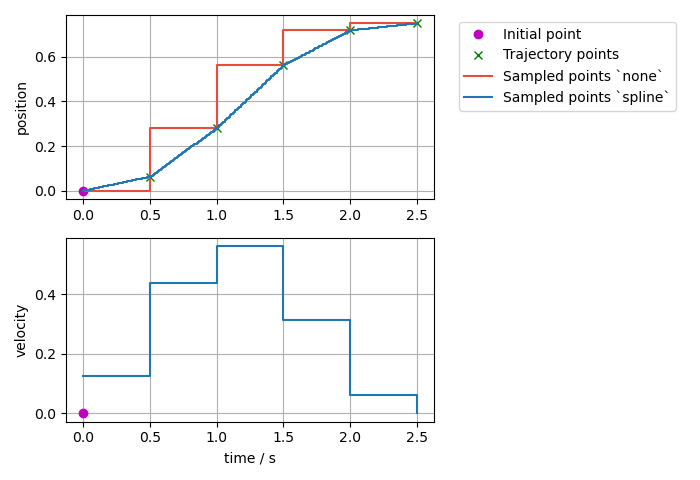
\includegraphics[width=130mm]{./fig/ros2_control/spline_position.png}
    %   \vspace{2mm}
    %   \caption{Joint-space trajectory for linear spline}\label{linear int}
    % \end{figure}

    \item Cubic: Position and velocity are specified so the continuity is confirmed at the velocity level.

    % \begin{figure}[h]
    %   \centering
    %   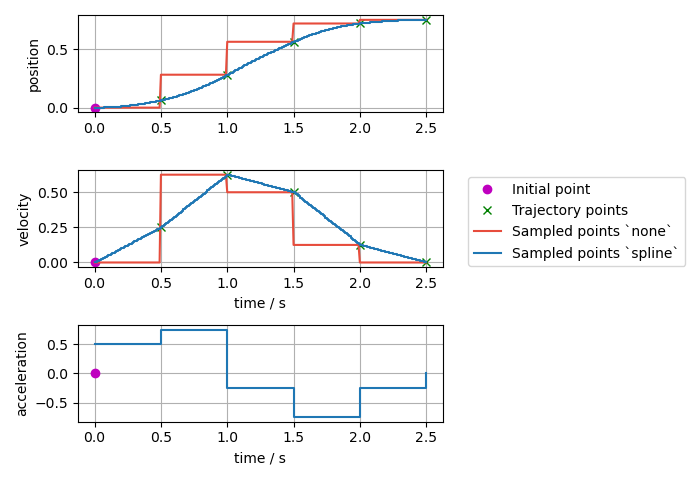
\includegraphics[width=130mm]{./fig/ros2_control/spline_position_velocity.png}
    %   \vspace{2mm}
    %   \caption{Joint-space trajectory for linear spline}\label{cubic int}
    % \end{figure}

    \item Quintic: Position, velocity and acceleration are specified: Guarantees continuity at the acceleration level.

    % \begin{figure}[h]
    %   \centering
    %   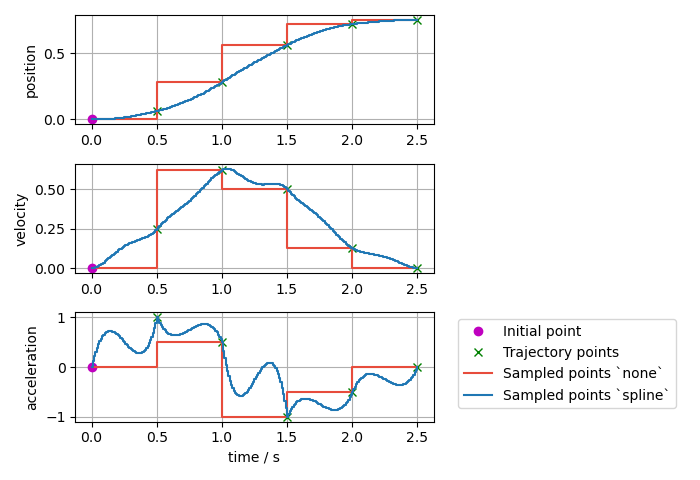
\includegraphics[width=130mm]{./fig/ros2_control/spline_position_velocity_acceleration.png}
    %   \vspace{2mm}
    %   \caption{Joint-space trajectory for linear spline}\label{quintic int}
    % \end{figure}
\end{itemize}

\begin{figure}[t]
 \begin{subfigure}{1.0\textwidth}
 \begin{center}
  \includegraphics[height=80mm]{./fig/ros2_control/jtc/spline_position.png}
\caption{Joint-space trajectory for linear spline.}\label{linear int}
 \end{center}
 \end{subfigure}
 
 \begin{subfigure}{0.5\textwidth}
 \begin{center}
  \includegraphics[height=80mm]{./fig/ros2_control/jtc/spline_position_velocity.png}
\caption{Joint-space trajectory for linear spline.}\label{cubic int}
\end{center}
\end{subfigure}
 \begin{subfigure}{0.5\textwidth}
 \begin{center}
  \includegraphics[height=80mm]{./fig/ros2_control/jtc/spline_position_velocity_acceleration.png}
\caption{Joint-space trajectory for linear spline.}\label{quintic int}
\label{subfig3}
 \end{center}
 \end{subfigure}
\vspace{-2mm}
\caption{Spline interpolation Strategies of joint trajectory controller.}
\label{interpolation}
\end{figure}

The joint-space trajectories for each case are illustrated in \fig{interpolation}. In this time, Moonbot is using only position linear interpolation for easier prototyping the motion control and designing gait motion.

\section{Gazebo Simulation}
Gazebo \cite{gazebo} stands as a robust open-source 3D simulation environment widely used in the robotics community. Its physics engine, sensor simulation, and realistic rendering capabilities make it a choice for testing Moonbot's motion and control strategies in both earth-based environment and lunar landscape environment.

%%%
\begin{figure}[t]
 \begin{subfigure}{0.5\textwidth}
 \begin{center}
  \includegraphics[width=78mm]{./fig/chap4/simulation/moonbot_gazebo.png}
\caption{Earth ground environment.}\label{subfig_gazebo1}
\end{center}
\end{subfigure}
 \begin{subfigure}{0.5\textwidth}
 \begin{center}
  \includegraphics[width=75mm]{./fig/chap4/simulation/moonbot_gazebo5.png}
\caption{Lunar surface environment.}\label{subfig_gazebo2}
 \end{center}
 \end{subfigure}
\vspace{-2mm}
\caption{Moonbot in Gazebo simulation.}
\label{gazebosim}
\end{figure}
%%%

\section{Kinematics Model of Legs Motion}

The inverse kinematics (IK) model is used as a function for calculate the joint positions, based on the given coordinates of the end effector's position in the leg's coordinate system.

Let $(x, y, z)$ represent the desired coordinates of the end effector position in the leg's coordinate system, as shown in \fig{leg_config}. The IK algorithm calculates the joint angles $(\theta_1, \theta_2, \theta_3)$ corresponding to the coxa, femur, and tibia joints, respectively. 

The result of coxa joint $(\theta_1)$, responsible for lateral movement, is limited within a span of -90 to 90 degrees. Similarly, the femur joint $(\theta_2)$, facilitating forward and backward motion, adheres to the same range of -90 to 90 degrees. Finally the tibia joint $(\theta_3)$ spans from -100 to 100 degrees. These specified limits ensure that the leg articulates within safe and mechanically feasible parameters.

\begin{figure}[h]
  \centering
  \includegraphics[width=120mm]{./fig/leg_configuration/IK.pdf}
  \vspace{2mm}
  \caption{Configuration of leg's module of Moonbot.}\label{leg_config}
\end{figure}

First, we initialize the parameters including the lengths of the leg segments ($l_1, l_2, l_3$) for coxa, femur, and tibia, respectively.

Inverse Kinematics Calculation:
    \begin{itemize}
      \item First, we calculate the distance from the coxa joint to the EE position in $xy$ plane, $l_{xy}$, and the distance from femur's joint to the end effector, $D_{j2E}$:
    
      \begin{equation} \label{l_xy}
        D_{xy} = \sqrt{x^2 + y^2}
      \end{equation}
      
      \begin{equation} \label{D_j2E}
        D_{j2E} = \sqrt{z^2 + (D_{xy} - l_1)^2}
      \end{equation}
      
      \item Calculate the angle ($\alpha$) between the femur segment and the line connecting the coxa and EE position:
      \begin{equation}
        \alpha = \arccos\left(\frac{l_3^2 - l_2^2 - D_{j2E}^2}{-2 \cdot l_2 \cdot D_{j2E}}\right)
      \end{equation}
      
      \item Calculate the joint angle ($\theta_1$) of the coxa joint:
      \begin{equation}
        \theta_1 = \arctan(y, x)
      \end{equation}
      
      \item Calculate the joint angle ($\theta_2$) of the femur joint:
      \begin{equation}
        \theta_2 = \arctan\left(\frac{z}{D_{xy} - l_1}\right) - \alpha
      \end{equation}
      
      \item Calculate the angle ($\beta$) between the tibia segment and the femur segment:
      \begin{equation}
        \beta = \arccos\left(\frac{D_{j2E} - l_2^2 - l_3^2}{-2 \cdot l_2 \cdot l_3}\right)
      \end{equation}
      
      \item Calculate the joint angle ($\theta_3$) of the tibia joint:
      \begin{equation}
        \theta_3 = \pi - \beta
      \end{equation}
    \end{itemize}
  
Return the calculated joint angles $(\theta_1, \theta_2, \theta_3)$ for the coxa, femur, and tibia joints, respectively. 


With the given leg segment lengths:
\begin{align}
  l_1 &= 64.55 \text{ mm} \\
  l_2 &= 129 \text{ mm} \\
  l_3 &= 156 \text{ mm}
\end{align}

the IK algorithm calculates the joint angles required to position the leg's end effector at the desired coordinates $(x, y, z)$ of the leg's frame.

Moonbot is also implemented with motion control in both translation and rotation around the axis. The rotation matrix $\mathbf{R(\theta_x, \theta_y, \theta_z)}$ is used to transform coordinates of the body's frame through matrix multiplication.

The elements of the rotation matrix are computed using the following expressions:

\vspace{2mm}
\begin{equation}
\mathbf{R}(\theta_x, \theta_y, \theta_z) = 
\begin{bmatrix}
c_ yc_z & s_x s_y c_z - c_x s_z & c_x s_y c_z + s_x s_z \\
c_y s_z & s_x s_y s_z + c_x c_z & c_x s_y s_z - s_x c_z \\
-s_y & s_x c_y & c_x c_y
\end{bmatrix}
\end{equation}
\vspace{2mm}

where $c_i$ represents cosine of $\theta_i$ and $s_i$ represents sine of $\theta_i$.

\section{Quadruped Operation}
The process of gait generation in legged locomotion is fundamental for achieving stable and efficient movement patterns. It involves determining the stride length and trajectory for each leg's step to maintain balance and driving force. Let's delve into the mathematics behind generating a gait for legged robots.

The control structure for the full configuration of Moonbot is depicted in Figure \fig{control}. Drawing inspiration from control strategies utilized in various quadruped and legged robots \cite{syropod}, \cite{uno2021hubrobo}, \cite{hyperdog}, Moonbot adheres to the classic approach for controlling quadruped robots.

At the low-level, an actuator interface serves as a bridge between user commands and the actual hardware. This interface, designed with the life cycle concept in ROS2, facilitates the transmission of commands to the motors while retrieving important feedback, including joint position, velocity, and torque.

End-effector control primarily focuses on solving the inverse kinematics problem to determine the joint positions corresponding to desired end-effector positions. The computed solutions are then forwarded to the appropriate controller based on the type of module in use.

Furthermore, the high-level controller encompasses a body motion planner and a gait generator, essential components for coordinating complex movements and locomotion patterns. Additionally, teleoperation control via a PS4 joystick has been implemented to provide manual control capabilities.\\

\begin{figure}[t]
  \centering
  \includegraphics[width=145mm]{./fig/flowchart/Controlcolor.png}
  \vspace{2mm}
  \caption{Control architecture for full configuration Moonbot.}\label{control}
\end{figure}


\subsection{Body Movement}
The body position control is managed by the body planner, which plays a critical role in maintaining balance during locomotion and in navigating uncertain terrain. \fig{slant} shows the translational movement of the body in four directions, while \fig{rot} depicts its rotation around three axes. \\

\begin{figure}[ht]
    \centering
    \begin{subfigure}[b]{0.45\textwidth}
        \centering
        \includegraphics[width=70mm]{./fig/chap4/body_movement/front05cmslant.JPG}
        \caption{Body moves 5 cm to the front.}
        \label{slantfront}
    \end{subfigure}
    \begin{subfigure}[b]{0.45\textwidth}
        \centering
        \includegraphics[width=70mm]{./fig/chap4/body_movement/back05cmslant.JPG}
        \caption{Body moves 5 cm to the back.}
        \label{slantback}
    \end{subfigure}
    \\
    \begin{subfigure}[b]{0.45\textwidth}
        \centering
        \includegraphics[width=70mm]{./fig/chap4/body_movement/left05cmslant.JPG}
        \caption{Body moves 5 cm to the left.}
        \label{slantleft}
    \end{subfigure}
    \begin{subfigure}[b]{0.45\textwidth}
        \centering
        \includegraphics[width=70mm]{./fig/chap4/body_movement/right05cmslant.JPG}
        \caption{Body moves 5 cm to the right.}
        \label{slantright}
    \end{subfigure}
    \caption{Body translational movement.}
    \label{slant}
\end{figure}

\begin{figure}[ht]
    \centering
    \begin{subfigure}[b]{0.45\textwidth}
        \centering
        \includegraphics[width=70mm]{./fig/chap4/body_movement/p05roll.JPG}
        \caption{Body rotates 5 degrees in roll.}
        \label{protroll}
    \end{subfigure}
    \begin{subfigure}[b]{0.45\textwidth}
        \centering
        \includegraphics[width=70mm]{./fig/chap4/body_movement/n05roll.JPG}
        \caption{Body rotates -5 degrees in roll.}
        \label{nrotroll}
    \end{subfigure}
    \\
    \begin{subfigure}[b]{0.45\textwidth}
        \centering
        \includegraphics[width=70mm]{./fig/chap4/body_movement/p05pitch.JPG}
        \caption{Body rotates 5 degrees in pitch.}
        \label{protpitch}
    \end{subfigure}
    \begin{subfigure}[b]{0.45\textwidth}
        \centering
        \includegraphics[width=70mm]{./fig/chap4/body_movement/n05pitch.JPG}
        \caption{Body rotates -5 degrees in pitch.}
        \label{nrotpitch}
    \end{subfigure}
    \\
    \begin{subfigure}[b]{0.45\textwidth}
        \centering
        \includegraphics[width=70mm]{./fig/chap4/body_movement/p10yaw.JPG}
        \caption{Body rotates 10 degrees in yaw.}
        \label{protyaw}
    \end{subfigure}
    \begin{subfigure}[b]{0.45\textwidth}
        \centering
        \includegraphics[width=70mm]{./fig/chap4/body_movement/n10yaw.JPG}
        \caption{Body rotates -10 degrees in yaw.}
        \label{nrotyaw}
    \end{subfigure}
    \caption{Body rotational movement.}
    \label{rot}
\end{figure}

\subsection{Gait Generation:}

\begin{enumerate}
    \item \textbf{End-effector Trajectory Generator}
    
\hspace{0.5cm}The trajectory of the legs step is calculated in the gait generator to perform gait patterns and stride vector. Each step along the trajectory involves determining the position of the leg. During the swing phase of each gait pattern, the leg's tip follows a sinusoidal trajectory. By iteratively computing the trajectory for each step, legged robots can generate stable and efficient gaits.

The trajectory equation for each step is given as:

\vspace{2mm}
\begin{equation}
    z(t) = \text{{$S$}} \times \sin\left(\frac{{\pi}}{{\text{{$L$}}}} \times \text{{$t$}}\right)
\end{equation}
\vspace{2mm}

where:
\begin{itemize}
    \item $S$ is step height.
    \item $L$ is step distance.
    \item $t$ is time step.
\end{itemize}

\begin{figure}[h]
  \centering
  \includegraphics[width=\linewidth]{./fig/chap4/stride/stride1.png}
  \vspace{2mm}
  \caption{Stride generation with sine function.}\label{stride}
\end{figure}

    \item \textbf{Gait Planner}
    
\hspace{0.5cm}With stride vector generation, gait planner plans the swing and stance phases of leg motion, enabling the generation of various gait patterns, including trot and dynamic crawl gait, as shown in Figure \fig{gait_diagram}. The timing of these gait cycles and the desired state of the leg are sent to the end effector's position controller to generate either swing or stance trajectory following the time step of the leg in the gait cycle. The series of snapshots for trot gait and crawl gait are presented in \fig{trotsnap} and \fig{crawlsnap}, respectively.
\end{enumerate}

% \subsection{Gait Generation}
\begin{figure}[t]
  \centering
  \includegraphics[width=\linewidth]{./fig/locomotion/diagram/gaitdiagram.pdf}
  \vspace{2mm}
  \caption{Gait diagram of walking motion.}\label{gait_diagram}
\end{figure}

\begin{figure}[t]
  \centering
  \begin{minipage}[b]{0.32\textwidth}
    \centering
    \includegraphics[clip, width=\linewidth]{./fig/chap4/gait/trot/t_step1.png}
  \end{minipage}
  \begin{minipage}[b]{0.32\textwidth}
    \centering
    \includegraphics[clip, width=\textwidth]{./fig/chap4/gait/trot/t_step2.png}
  \end{minipage}
  \begin{minipage}[b]{0.32\textwidth}
    \centering
    \includegraphics[clip, width=\textwidth]{./fig/chap4/gait/trot/t_step3.png}
  \end{minipage}\\
  \begin{minipage}[b]{0.32\textwidth}
    \centering
    \includegraphics[clip, width=\textwidth]{./fig/chap4/gait/trot/t_step4.png}
  \end{minipage}
  \begin{minipage}[b]{0.32\textwidth}
    \centering
    \includegraphics[clip, width=\textwidth]{./fig/chap4/gait/trot/t_step5.png}
  \end{minipage}
  \begin{minipage}[b]{0.32\textwidth}
    \centering
    \includegraphics[clip, width=\textwidth]{./fig/chap4/gait/trot/t_step6.png}
  \end{minipage}\\
\caption{Series pictures of Moonbot walking with trot gait towards the top of the page. The pictures were taken every 1 sex from left to right, top to bottom.}
\label{trotsnap}
\end{figure}

\begin{figure}[t]
  \centering
  \begin{minipage}[b]{0.32\textwidth}
    \centering
    \includegraphics[clip, width=\linewidth]{./fig/chap4/gait/crawl/c_zmp1.png}
  \end{minipage}
  \begin{minipage}[b]{0.32\textwidth}
    \centering
    \includegraphics[clip, width=\textwidth]{./fig/chap4/gait/crawl/c_step1.png}
  \end{minipage}
  \begin{minipage}[b]{0.32\textwidth}
    \centering
    \includegraphics[clip, width=\textwidth]{./fig/chap4/gait/crawl/c_step2.png}
  \end{minipage}\\
  \begin{minipage}[b]{0.32\textwidth}
    \centering
    \includegraphics[clip, width=\textwidth]{./fig/chap4/gait/crawl/c_zmp2.png}
  \end{minipage}
  \begin{minipage}[b]{0.32\textwidth}
    \centering
    \includegraphics[clip, width=\textwidth]{./fig/chap4/gait/crawl/c_step3.png}
  \end{minipage}
  \begin{minipage}[b]{0.32\textwidth}
    \centering
    \includegraphics[clip, width=\textwidth]{./fig/chap4/gait/crawl/c_step4.png}
  \end{minipage}\\
\caption{Series pictures of Moonbot walking with crawl gait towards the top of the page. The pictures were taken every 1 sex from left to right, top to bottom.}
\label{crawlsnap}
\end{figure}

%%% EOF %%%

\chapter{Conclusions}
%\label{cha:DDDD}
%%%%%%%%%%%%%%%%%%%%%%%%%%%%%%%%%%%%%%%%%%%%%%%%%%%%%%%%%
%%%
%%%  第5章
%%%  結論
%%%
%%%%%%%%%%%%%%%%%%%%%%%%%%%%%%%%%%%%%%%%%%%%%%%%%%%%%%%%%
\section{Conclusion}

In this research, we have focused on the development of self-recognition and modular control capabilities for Moonbot, a modular legged robot. By providing adaptability to different configurations, Moonbot uses internal sensor to demonstrate the ability to recognize itself and its potential to operate in various configurations. The ROS2-based control framework implemented enables seamless integration of different modules and additional sensors, paving the way for future advancements in Moonbot's capabilities.

Furthermore, the development of a high-level controller for Moonbot's quadruped configuration, both in simulation and real-world scenarios, showcases its operational versatility and robustness. These achievements mark significant milestones towards autonomous and adaptable robotic systems for lunar exploration and beyond.

\section{Future Improvements Plan}

Looking ahead, future work will focus on enhancing Moonbot's control strategies and adaptability through the implementation of reinforcement learning (RL) algorithms, particularly tailored for the lunar surface environment. RL has shown promise in enabling robots to learn and adapt to complex and dynamic environments by continuously improving their decision-making processes based on feedback from the environment. In the context of legged robots, RL algorithms can be utilized to optimize locomotion patterns and adapt to varying terrain conditions, ultimately enhancing the robot's mobility and efficiency. Many researchers have driven into this new strategies to control legged robot, for example, Anymal from ETH Zurich \cite{anymalRL}, \cite{anymalDRL}.

\begin{figure}[t]
  \centering
  \includegraphics[width=140mm]{./fig/chap5/isaacgym.jpg}
  \vspace{2mm}
  \caption{Anymal robot walking training in Isaac Gym environment. \cite{legged_gym_git}}\label{anymalgym}
\end{figure}

Furthermore, in the modularity side, the application of deep reinforcement learning (DRL) algorithms will be investigated to optimize the design process of modular legged robots \cite{modularDRL}, \cite{modularlegDRL}. DRL techniques, which leverage deep neural networks to approximate complex functions, offer the potential to revolutionize the way legged robots are designed and controlled. By using DRL, Moonbot and similar robots can autonomously learn and refine their locomotion strategies, leading to more agile and robust robotic systems.\\

% \begin{figure}[ht]
%   \centering
%   \includegraphics[width=90mm]{./fig/chap5/modularDRL.png}
%   \vspace{2mm}
%   \caption{Modular manipulator design tree, synthesized by deep reinforcement learning. \cite{modularDRL}}\label{modularDRL}
% \end{figure}



The integration of reinforcement learning techniques into the control and design processes of modular legged robots represents a significant step towards achieving autonomous operation in challenging environments, such as lunar surfaces. By leveraging RL and DRL algorithms, Moonbot and future generations of legged robots can overcome obstacles, navigate complex terrains, and accomplish tasks with greater efficiency and adaptability.

In conclusion, the combination of reinforcement learning, modular robotics, and space exploration holds immense potential for advancing the field of robotics and unlocking new capabilities for autonomous systems. By bridging the gap between theoretical research and practical application, we can pave the way for the next generation of robotic explorers, capable of operating effectively in the harsh and unpredictable environments of space.

\begin{figure}[t]
    \centering
    \begin{subfigure}{1.0\textwidth}
        \centering
        \includegraphics[width=140mm]{./fig/chap5/modularlegDRLtree.png}
        \caption{Design space tree for modular mobile robot, using deep neural network.}
        \label{moduleDRLtree}
    \end{subfigure}
    % \hfill
    \\
    \begin{subfigure}{1.0\textwidth}
        \centering
        \includegraphics[width=140mm]{./fig/chap5/modularlegDRL.png}
        \caption{Evaluation of modular designs in simulation across terrains of varying roughness, showcasing the adaptability of different robot configurations.}
        \label{modularDRL}
    \end{subfigure}
    \vspace{2mm}
    \caption{Modular mobile robot design selection with deep reinforcement learning. \cite{modularlegDRL}}
    \label{DRLmodular}
\end{figure}


%%% EOF %%%

%%%%%%%%%%%%%%%%%%%%
%%%   参考文献
%%%%%%%%%%%%%%%%%%%%

%%%%%%%%%%%%%%%%%%%%%%%%%%%%%%%%%%%%%%%
%%%  2020.01.08 modified by Kentaro UNO
%%%  pBibtexを使ったものに書き換え
%%%%%%%%%%%%%%%%%%%%%%%%%%%%%%%%%%%%%%%
%%% 以下の二行がないとhyper linkがずれる.
\cleardoublepage %jbookクラスなどにおいて必ず奇数ページからはじまるように改ページする. 
\phantomsection %空の仮想セクションをおいて「Linkずれ」を回避.
\addcontentsline{toc}{chapter}{Bibliography}
%% 

\begin{thebibliography}{99}
\itemsep 3mm{
	
	%著者1,著者2:`` 題目 '',学会名(出版社),西暦
	%
	%author1, author2: `` title '', conference, year
	
	%\bibitem{}
	%	氏 名:
	%	`` 題目 '',
	%	学会名(出版社),
	%	西暦

	\bibitem{GLXP}
	Google Lunar XPRIZE公式ホームページ, http://lunar.xprize.org/

	\bibitem{hakuto}
	チームHAKUTO公式ホームページ, http://team-hakuto.jp/

	\bibitem{lava-tube1}
		Haruyama J., Sawai S., Mizuno T., Yoshimitsu T., Fukuda S., Nakatani I., 
			``Exploration of Lunar Holes, Possible Skylights of Underlying Lava Tubes, by Smart Lander for Investigating Moon (SLIM)'',
				Transactions of the Japan Society for Aeronautical and Space Sciences, Aerospace Technology Japan, vol. 10, pp. Pk\_7-Pk\_10, 2012.

	\bibitem{lava-tube2}
		Samuel J., Julie D., B. Ray Hawke, Benjamin T., Joshua T. S., Joshua L., Bradley L., Brett W., Mark S., Timothy D., D. Benjamin J., Paul D., Thomas A., W. Brent Garry, 
			``LRO observations of morphology and surface roughness of volcanic cones and lobate lava flows in the Marius Hills'', Journal of Geophysical Research, Volume 118, Issue 4, pp. 615-634, 2013.

	\bibitem{HAKUTOmission}
		Britton N., Yoshida K., Walker J., Nagatani K., Taylor G., Dauphin L., 
			``Lunar micro rover design for exploration through virtual reality tele-operation'', 
				Proceedings of the 9th Conference on Field Service and Robotics, pp. 1-14, 2013.

	\bibitem{ToFprinciple}
		Miles H., Seungkyu L., Ouk C., Radu H., 
			{\it ``Time of Flight Cameras: Methods, and Applications''}, 
				Springer, 2012.

	\bibitem{robotToF}
	Stephan H., Thorsten L., 
		``Robot Vision System based on a 3D-TOF Camera'', 
			Proceedings of IEEE Instrumentation \& Measurement Technology Conference IMTC, pp. 1-5, 2007.	

	\bibitem{robotToF2}
	Guillem A., Sergi F., Carme T.,
		``ToF Cameras for active vision in robotics'', 
			Sensors and Actuators A: Physical, Volume 218, pp. 10-22, 2014.

	\bibitem{Takuto-san-paper}
	Oikawa T., Tanaka T., Walker J., Uno K., Costa P., Britton N., Yoshida K.,
		``Thermal design and analysis of conceptual fright model of lunar exploration rover'', 
			Proceedings of the 13th i-SAIRAS, 2016.

	\bibitem{reflectance_of_regolith}
		Heiken G.H., Vaniman D.T., French B.M., 
			{\it ``Lunar Source book''}, 
				Cambridge University Press, 1991.	
	
	\bibitem{solar-irradiance}
		Hulstrom R., Bird R., Riordan C., 
			``Spectral solar irradiance data sets for selected terrestrial conditions'', 
				Solar Cells, Volume 15, pp. 365-391, 1985.

	\bibitem{Higa-san-paper}
		Higa S., Nagaoka K., Yoshida K., 
			``Online estimation of wheel sinkage and slippage using a ToF camera on loose soil'', 
			 Proceedings of the ISTVS 8th Americas Regional Conference, accepted, 2016.

	\bibitem{NIST}
		NIST, Standard Test Methods For Response Robot, ``Guide for Evaluating, Purchasing, and Training with Response Robots Using DHS-NIST-ASTM International Standard Test Method'', https://www.nist.gov/programs-projects/department-homeland-security-response-robot-performance-standards (accessed on 9/2/2016).
		


}
\end{thebibliography}


\bibliographystyle{./include/junsrtForThesis} %use customized Bibtex style file. 2020.01.08 modified by Kentaro UNO
\bibliography{./bibtex/reference}

%%%%%%%%%%%%%%%%%%%%
%%%   謝辞   
%%%%%%%%%%%%%%%%%%%%
\cleardoublepage
\phantomsection
\addcontentsline{toc}{chapter}{Acknowledgements}
%%%%%%%%%%%%%%%%%%%%%%%%%%%%%%%%%%%%%%%%%%%%%%%%%%%%%%%%%
%%%
%%%  謝辞
%%%
%%%%%%%%%%%%%%%%%%%%%%%%%%%%%%%%%%%%%%%%%%%%%%%%%%%%%%%%%
\begin{my_ack}
This book was created at the Space Robotics Laboratory, Faculty of Engineering, Tohoku University and supported by JST Moonshot R\&D Program, Grant Number JPMJMS223B.

I extend my sincere appreciation to the Space Robotics Laboratory of Prof. Kazuya Yoshida, where I have had the privilege of conducting my research. I am deeply grateful for the mentorship, guidance, and opportunities provided by Prof. Yoshida and the lab members, which have been invaluable to my growth and development in the field of robotics.

I am indebted to Assistant Prof. Uno Kentaro and Prof. Shreya Santra for their invaluable support and guidance throughout my journey. Assistant Prof. Uno's insights and advice on legged robotics have been instrumental in shaping my understanding of this complex field, while Prof. Shreya's support in ideation and thesis writing has been invaluable.

I would like to express my heartfelt thanks to Danish AI for his exceptional work in developing the hardware design of Moonbot. Additionally, I extend my gratitude to Pascal Pama and Torii Keigo for their support during experiments and their insightful comments on my work.

Special thanks are due to Gustavo Diaz for his significant contributions to Moonshot project team. His advice on robot software development and debugging has been invaluable to our progress.

I am deeply grateful to the Limbing Robotics team for their invaluable contributions to my understanding of legged robotics. Their expertise and knowledge-sharing have been instrumental in shaping my understanding of this complex field. Special thanks are due to the Limbero climbing quadruped robot team, whose insights and advice on Moonbot's software development have been invaluable to our project's success.

I would also like to express my sincere appreciation to Uchida Akiyoshi of the Orbital Robotics team for his assistance with ROS2 control. His guidance and support have been instrumental in navigating the intricacies of robotic control systems, enabling us to enhance Moonbot's capabilities.

Additionally, I extend my gratitude to Nagaoka Keita for his support with video shooting, which has been essential in documenting and sharing our project's progress effectively.

To each of these individuals and teams, I offer my deepest thanks for their invaluable contributions, guidance, and support, which have significantly enriched my journey in robotics and contributed to the success of the Moonshot project.

\begin{flushright}
February, 2024\\
Tharit Sinsunthorn
\end{flushright}
\end{my_ack}
%%%  EOF %%% % \begin{my_ack} を使用する.

%%%%%%%%%%%%%%%%%%%%
%%%   Appendix
%%%%%%%%%%%%%%%%%%%%
% \cleardoublepage
% \phantomsection
% \addcontentsline{toc}{chapter}{Appendix}
% \appendix
% \chapter{Appendix}
% \label{cha:appendix}
% %%%%%%%%%%%%%%%%%%%%%%%%%%%%%%%%%%%%%%%%%%%%%%%%%%%%%%%%%
%%%
%%%  Appendix
%%%
%%%%%%%%%%%%%%%%%%%%%%%%%%%%%%%%%%%%%%%%%%%%%%%%%%%%%%%%%
\section{Section title for appendix}

%%% EOF %%%

\end{document}

